\chapter{Optimal Design for Estimation in SDEs}
\label{ch:optimal_design}
\graphicspath{{../OptEstimate/}}
<<<<<<< HEAD
=======

\usepackage{amsfonts}
\usepackage{mathrsfs}

>>>>>>> 6d1ee3c9eb52b6bed66343a6488d0f9a4ca3aef0
% DEFINITIONS:
\def \Prob 	  {{ \mathbbmtt{P}  }} %the expectation operator
\def \th 	  {{ \theta}}
\def \FI 		{{\Phi}}
\def \KL     {{ K\!L}}

\def \adot {{ \dot{\alpha} }}
\def \Udot {{ \dot{U}}}
\def \In	{{ i_n}}
\def \vt 	{{ v_{\textrm{th} } }}
\def \Ihat  {{ \hat{I}  }}
\def \p 	{{ \phi  }}

\def \G		{{ \bar{G}  }} %{{ \reflectbox{G} }}
\def \Gest  {{ \hat{\G} }}
\def \Gtilde		{{ \tilde{\G} }}
\def \D		{{ \reflectbox{D} }}
\def \dphi {{ \delta \phi }}

\def \L {{ \Lambda }}
\def \P {{ \Phi }}
\def \n {{\nu}}
\def \Fx {{ F_x}}
\def \Fxx {{ F_{xx} }}
\def \Ft {{ F_t }}
\def \xest {{ \hat{x}_t}}
\def \muncond {{ {m}_x}}
\def \mcond {{ {m}_x^c}}

\def \f {{\rho}}
\def \F {{\Phi}}
\def \Fn {{\mathcal{F}}}

\def \abg		{{\a,\b,\g }} 
\def \aest      {{ \hat{\a} }}
\def \best      {{ \hat{\b} }}
\def \gest      {{ \hat{\g} }}
\def \estabg	{{\aest, \best, \gest}}
\def \abgest	{{\estabg }}

\def \sAlg {{ \mathcal{A} }}
\def \N {{ \mathcal{N} }}
\def \Udomain {{ \mathcal{U} }}
\def \Umax {{ u_{\textrm{max}} }}
\def \umax	{{ u_{\textrm{max}} }}
\def \amin	{{ \a_{\textrm{min}} }}
\def \amax	{{ \a_{\textrm{max}} }}
\def \astar {{ \a^* }}
\def \xth	{{ x_{th} }} 
\def \yth	{{ y_{th} }}
\def \xmin	{{ x_{-} }}
\def \xmax	{{ x_{+} }}
\def \xmid  {{ x_{mid} }}

% \def \x {{ \boldsymbol{x} }}
% \def \u {{ \boldsymbol{u} }}
% \def \p {{ \boldsymbol{p} }}
% \def \q {{ \boldsymbol{Q} }}
% \def \f {{ \boldsymbol{f} }}
\def \tf {{ t_f }}
\def \tc {{ \tau_{c} }}
\def \lc {{ \lambda_{c} }}
\def \ts {{ t_{\textrm{sp} } }}
\def \tn {{ t_n }}
\def \tns {{ \{t_n \} }}
\def \T {{ T^*  }}

\def \free {{\textrm{free} }}


\def \Ttwo {{ \hat{T}_{(2)} }}
\def \Ttwol {{ \hat{T}^{\lambda}_{(2)} }}
\def \Tone {{ \hat{T}_{(1)} }}
\def \Ti {{ \hat{T}_{(i)} }}

\def \Normal {{ \mathcal{N} }}
\def \L {{ \mathcal{L} }}
\def \Lstar {{ \L^* }}
\def \H {{ \mathcal{H} }}
\def \dx {{ \delta\! x}}
\def \da {{ \delta\! \a}}
\def \df {{ \delta\! f}}

% COMP EXAM:
\def \Lonepm {{\mathbb{L}^1}}
\def \Ltwopm {{\mathbb{L}^2}}
\def \Fil 	{{\mathcal{F}}}

\def \x {{ \vec{x} }}
\def \X {{ \vec{X} }}
<<<<<<< HEAD
% parameterized densities / adjoints:
\def \ft {{ f_\th}}
\def \pt {{ p_\th}}
\def \dft {{ \delta f_\th}}
\def \wt {{ w_\th }}

\def \aopt {{\a_{opt} }}
=======

>>>>>>> 6d1ee3c9eb52b6bed66343a6488d0f9a4ca3aef0


% \def\input@path{{../OptEstimate}} 
%TODO: change to consistent notation:
% TODO: Fix the .txt includes
 
\section{Thesis Context}
 In the last of the three main chapters of the thesis, we discuss the problem of
 stimulating a neuron model system in order to obtain higher fidelity model
 parameter estimates. We use the Mutual Information as the formal criterion for optimization. Since the
 parameters of the system are not known, we demonstrate why it is impossible to derive a HJB equation for the
 optimization problem in the full-observation case. However, one can still
 derive a variational, Maximum-Principle-based iterative schema to obtain the
 optimal stimulus. We then use this to find the optimal stimulation and perform
 several simulated estimations to demonstrate the superiority of the
 MI-optimal control over common-sense alternatives.
 
 This chapter can be seen to combine many of the features of the previous two
 chapters - we are again trying to control spike-times as in the second chapter,
 but with the ultimate goal of estimating parameters from the spike observations
 as in the first. Mathemtaically the greatest difference between the
 optimization problem in this chapter and that in the second is that we no
 longer assume a definite single set of model parameters, but instead must work
 with {\sl distributions} over the parameters. This renders the problem more
 difficult and in particular makes the adjoint derivations more complex. Instead
 of a single-pair of forward-backward PDEs, we now must deal with a ensemble of
 loosely coupled forward-backward PDEs.
  
    
\section{Introduction}
We consider the problem of optimal design for estimation of parameters in a
stochastic differential equation (SDE) given only observations of hitting times
from the SDE. We assume that the 'controller' has influence over some part of
the parameters of the SDE and the objective is to obtain observations that are
most informative in both formal and informal senses. That is, we choose the
control as the solution to a well-posed optimization problem, but our ultimate
goal is to obtain more accurate and more precise estimates of the unknown
parameter(s) given the observed hitting times.

We espouse a Bayesian perspective and proceed by assuming a prior
distribution of the unknown parameters. Then we seek to maximize the Mutual
Information (MI) between the posterior of the unknown parameters given the
observations and the distribution of the hitting times. Note that even for a
fixed and known parameter set the resulting observations, i.e.\ the hitting
times, are still random, due to the inherent stochasticity of the SDE. 

Using Mutual Information for the selection of 'maximally informative'
experiments has been advocated by several recent lines of research, for example,
in experimental psychology, \cite{Cavagnaro2010,Myung2013}, computational
neuroscience \cite{Paninski2006a,Paninski2005,Lewi2009} and quantum physics,
\cite{Granade2012}.
 
An alternative approach is to maximize the Expected Fisher Information of the
experiment, see \cite{Hooker2015}, which is especially effective if the Fisher
Information of the parameter estimators is available as an analytical formula.
That is the case when one observes full trajectories from the diffusion process,
as in \cite{Hooker2015}, but not in the more limited hitting-times observations
context.
 
The Mutual Information measures the expected reduction in uncertainty in the
parameter value given an observation, under a fixed experimental stimulation.
Thus the stimulation that maximizes the Mutual Information should extract the
maximum information about the model's parameters, on average. Using Mutual
Information for estimating statistical quantities is formally justified by
\cite{Paninski2005}, where proofs are provided showing that given fairly weak
modeling conditions, using a stimulation that iteratively maximizes the mutual
information between future observations and the parameters of interest leads to
consistent and efficient parameter estimates. However, while theoretically
sound, optimizing or even merely computing the Mutual Information may be
computationally prohibitive. For our problem of interest though, that is not a
primary issue.

We should explicitly single out a very recent paper on estimation
parameters in a quantum system,  
\cite{Granade2012}, where the authors describe a strategy to estimate
the parameters of the Hamiltonian of a quantum experiment. They use a simple
filtering technique originally suggested by \cite{Liu2001} to maintain and
update the prior distribution of the unknown parameters. In principle, their
approach is quite similar to ours, the main difference is the nature of the
observations, which in our case are the hitting times.

As posed, our optimization problem reduces to a slightly non-standard Partial
Differential Equation (PDE) optimization problem, in particular a Fokker-Planck
optimization problem. The field of PDE optimization is vast and we can just
mention one of many good references, \cite{Borzi2012}. There have recently
appeared a series of articles on Fokker-Planck based PDE-optimization, e.g.
\cite{Annunziato2010,Annunziato2014}. None of these however deal with the
boundary term that arises out of the hitting-time-based objective. We
should also mention our own work, \cite{Iolov2014a}, where we again solve a
hitting-time inspired optimization problem. The fundamental difference here is
that the uncertainty in the model parameters renders the problem more
complicated as it necessitates us to solve a system of (loosely-) coupled PDEs
rather than just one as in \cite{Iolov2014a}.

Our paper is also part of the general literature on estimating parameters of
diffusion processes from hitting-times observations only. Partly due to the
applications of this problem in theoretical neuroscience a lot has been written
on the subject for example in
\cite{Ditlevsen2007,MullowneyIyengar2008,Alili2005} and our own \cite{Iolov2013}
where we deal with the more exotic case of a sinusoidal driving force. The
literature on estimation from hitting-times of the class of diffusion models we
consider is clear that one parameter in particular, the characteristic time, is
most difficult to estimate having the widest confidence bounds by far. Thus we
focus on devising stimulations that will render most accurate estimations for
this parameter assuming that the other parameters are known or at least
nominally known in a sense that we explain later. In fact, we show that even if
the other parameters are also to-be estimated, for this problem, a control
designed with the goal of estimating the characteristic time parameter only,
ends up helping estimate all parameters.  

Thus our paper can be summarized as solving a PDE-optimzation arising from
maximizing the Mutual Information between a prior of the characteristic time
parameter and the random (future) hitting-times. The paper outline is as
follows: in \cref{sec:problem_formulation} we describe the mathematical formulation of the optimal design problem; in
\cref{sec:maximizing_MI}, we describe the optimization procedure, in particular
the derivation of the objective gradient and the numerical methods used; in
\cref{sec:batch_estimation}, we show the performance of the optimally designed
stimulation when many observations are first collected and only a single-pass,
{\sl batch} estimation is performed afterwards; in \cref{sec:online_estimation},
we turn to the {\sl online} problem, where the estimation is performed
after each observation and the stimulation is adjusted to reflect the newly
updated prior of the unknown parameters; in \cref{sec:discussion} we make
concluding and forward-looking remarks.

 
\section{Problem Formulation}
\label{sec:problem_formulation}
We would like to estimate the parameters in a noisy, leaky integrate-and-fire
(LIF) neuronal model. This is a diffusion process that has an absorbing barrier
at at an upper boundary and is unbounded below. In particular it is governed by,
\begin{equation}
\begin{gathered}
dX_t = \left(\underbrace{\a(t)}_{\textrm{control}} + \frac 1\tc(\m %\g \sin(\ot)
 - {X_t} ) \right) \intd{s} + \s\intd{W_t},
\\
X(0) = 0,
\\
X(\ts) = \xth \implies  
\begin{cases}
X(\ts^+) &= 0   
\\
t_k &=  \ts
\\
k  &= k+1
\end{cases}
\end{gathered} 
\label{eq:X_evolution_uo_control}
\end{equation}
The 'hitting time', $\ts$ is the first-time the process touches the upper
boundary, $\xth$, which is here set to $\xth=1$. Once a hitting-time is
recorded, the process is reset to $0$ and then continues from there. The control
$\a(t)$ is arbitrary and can be altered at any time; however, the parameter set,
$\th = \{\m, \tc, \s\}$, is assumed to be constant.

In the context of parameter estimation, we will assume that (a subset of) the
parameter set $\th = \{\m, \tc, \s\}$ is unknown and only the hitting times,
$\{t_k\}$, are observable.

In fact, we will concentrate on estimating the characteristic time ($\tc$). As
we mentioned in the introduction, previous papers on estimating parameters of
LIF from hitting times, e.g.\ \cite{Ditlevsen2007,MullowneyIyengar2008}, have
at length discussed that the estimation of $\tau$ is clearly the
hardest. In fact the literature is still not quite in agreement whether $\tau$ is hard to estimate or
whether it is simply unidentifiable. Since these studies were done in the
context of no control $\a=0$ or at least $\a= \textrm{const}$, we posit that
a judicious choice for the shape of $\a$ can significantly improve the
estimation of $\tau$.

Our goal is to choose the control, $\a(t)$, such as to 'best' estimate $\tc$
given only that the spike times $\{t_k\}$ are observed. Equivalently, setting
$t_0 = 0$, we can talk about the inter-spike intervals, $\{S_k\}$, which are
just the differences of subsequent spike times, $S_k = t_k - t_{k-1}$.

The probability density of the length of the $k$th interval,
conditional on some applied control $\a(\cdot)$, will be denoted as
\begin{equation} 
\begin{array}{rcll} 
g_k(t) \intd{t} &:=& \Prob[I_{k} \in [t, t + \intd{t})  \,|\,
 \a(\cdot)] &
 \textrm{(probability density)} 
% \\ 
% G_{n}(t) &:=& \Prob \left[T_{n} \leq t  \,|\,
%  \a(\cdot) \right] = \int_0^t g_{\phi}(\t) \intd{\t} &
%  \textrm{(cumulative distribution)}
% \\
% \G_{n}(t) &:= & \Prob(T_{n}>t \,|\, \a(\cdot) ) = 1 - G_{n}(t)
% &
%  \textrm{(survivor distribution)}
\end{array}
\label{eq:ISI_distribution_functions}
\end{equation}
We will drop the hitting-time indexing subscript, $k$, when there is no
confusion. 

The transition density for the state variable, $X_t$, $t \in [0, I_{n})$, will
be denoted as
\begin{equation}
f(x,t) := \Prob \left[X_{t} \in [x, x+ \intd{x})  \,|\,
 X_0 = 0, X_{s < t} < 1  \right]  \quad
 \textrm{(transition density)}
 \label{eq:transition_distribution}
\end{equation} 
The transition density satisfies a Fokker-Planck PDE over the domain, $x \in
(-\inf, \xth]$
\begin{equation}
\begin{gathered}
\begin{array}{lcl}
	\di_t f (x,t) &=&
					\underbrace{\frac{\s^2 }{2}}_{D}\cdot \di^2_x f 
					+ \di_x \Bigg(  
					\underbrace{\Big( \frac 1\tc (x-\m) - \a(t) \Big)}_{U(x,t)}  \cdot  f
					\Bigg)
					\\
					&=&
					D \cdot \di^2_x f +
					\di_x  \Big( U(x,t) \cdot f \Big)
					\\
					&=&
					- \di_x \phi(x,t)
					\\
					&=&
					\L[f] 
					\end{array}
	\\
	\left\{ \begin{array}{lcl}
	 f (x,0) &=& \delta(x)
	\\
	D \di_xf + U f |_{x=\xmin} &=& 0 
	\\
	f |_{x=\xth} &=& 0.
	\end{array} \right.
\label{eq:FP_pde_OU_absorbBC}
\end{gathered}
\end{equation}

The probability flux-out at the threshold boundary, $\phi(\xth, t)$, is very
important as it is related to the spike-time density,
\cref{eq:ISI_distribution_functions} via 
$$g(t)  = \phi(\xth, t) = -D\cdot \di_x
f|_{x=\xth}.$$
Recall that $U \cdot f = 0$ at the absorbing boundary, $\xth$.


%  In a typical (maximum likelihood) estimation experiment, we will see a lot of
% spikes and form the likelihood as $$ L(\th| t_n ) = \prod_n g_n(t_n) $$ We
% will then take logs and proceed as usual: $$ l(\th| t_n ) = \sum_n \log
% (g_n(t_n)) =  \sum_n \log ( -\di_t F(1,t_n)) $$ and then maximize $l$ over the
% parameters $\th$.  The associated {\sl score} function is $$ S(\th | \ts ) =
% \grad_\th l(\th | \ts) $$ The score function is a vector\footnote{We write
% $\grad$ for the vector differential and $\di$ for its scalar components, i.e.\
% $\grad_\th = [\di_{\th_1},\ldots\di_{\th_i}],\ldots$}.  The typical Maximum
% Likelihood process is to maximize the likelihood, $l$ which, if one uses a
% gradient-based approach amounts to finding the roots of the score, $S$.

In our Bayesian approach, we assume some {\sl  prior} distribution over
the possible values of $\th$. We denote the prior distribution as
$$
\begin{array}{rcll} 
\rho(\th) \intd{\th} &:=& \Prob(\Theta \in [\th, \th + \intd{\th})  ] &
 \textrm{(prior density)} 
 \end{array}
$$.

Given a single observation, $\ts$, the parameter posterior 
distribution is 
\begin{equation}
p(\th| \ts; \a) =
\frac{g(\ts |\th; \a)\cdot \rho(\th)}{\int_\Theta g(\ts|\th; \a)\cdot \rho(\th)
\intd{\th}}
\label{eq:parameter_posterior_defn}
\end{equation} 
Where $ g( \ts |\th; \a)$ is the likelihood of the hitting time given in
\cref{eq:ISI_distribution_functions}.

Our goal is to choose the control, $\a(\cdot)$, that maximizes the mutual
information  between the two random variables, $\Th, \ts$. Conditional on
$\a(\cdot)$, the Mutual Information, $I$, is given by
\begin{equation}
I[\a]= 
\int_\Theta \int_0^\infty g(t|\th)\rho(\th) \cdot 
\log \left( \frac{g(t|\th)}
{\int_\Theta g(t|\th)\rho(\th) \intd{\th}   } \right)
\intd{t}\intd{\th}.
\label{eq:J_mutual_info_objective}
\end{equation}

See \cref{sec:mutual_info_defn} for how this is derived from the usual textbook
definition of the Mutual Information. For different controls, $\a(\cdot)$,
the mutual information, $I$, will be different since $g$, the hitting time
density depends on the shape of $\a$ (the prior, $\rho$, does not). 
  
In short, we want to find the control input $\a(\cdot)$, which maximizes $I$ in
\cref{eq:J_mutual_info_objective} and we then verify that observations obtained
under such 'optimal' stimulation lead to parameter estimates that are more
accurate and more precise than parameters obtained for observations when the
system is perturbed by 'sub-optimal' stimulations.

\section{Maximizing the Mutual Information,
\cref{eq:J_mutual_info_objective}, using the Adjoint Method}
\label{sec:maximizing_MI}
Let us discuss the optimization problem
$$
\a(\cdot) = \argmax_{\a \sim \textrm{admissible}} I[\a]
$$ 

in our case, admissible controls are simply those that are continuous and with
the upper and lower bounds, $\a(t) \in [\amin, \amax] \,  \forall t$.

Our goal will be to obtain the gradient of $I$ with respect to $\a$, and then
use it in a standard gradient-based optimization procedure. There is the added
complexity that the gradient here is an infinite dimensional object and there
are some subtle functional analysis questions from a purely mathematical
point-of-view, we refer to the references, \cite{Lenhart2007,Borzi2012} for
rigorous justification of the manipulations. 

To proceed with obtaining the gradient with respect to $\a$, let us rewrite \cref{eq:J_mutual_info_objective}) in terms of the transition density, $f$. 
\begin{equation}
I[\a] = 
- \int_\Theta \int_0^\infty
	   \di_xf_\th(\xth, t|\th)  \rho(\th) \cdot 
		\log \left( \frac{\di_xf_\th(\xth, t|\th)}
						{\int_\Theta \di_xf_\th(\xth, t|\th)\rho(\th)
\intd{\th} } \right)
\intd{t}\intd{\th}
\label{eq:I_mutual_info_objective_in_terms_of_dixf} 
\end{equation}
We have dropped the constant, $D$ from
\cref{eq:I_mutual_info_objective_in_terms_of_dixf} as it is irrelevant for
the maximizing value of $\a$.

 In a standard approach for what
is known as the {\sl adjoint}  method of deriving a gradient of a
functional of a solution to a PDE with respect to one of the PDE's inputs, we
augment the objective, $I$, with the dynamics of $f$, by introducing the {\sl
adjoint} variable, $p$: 
\begin{align}
I=&  -
\int_\Theta \int_0^\infty 
	  \di_xf_\th(\xth, t|\th)  \rho(\th) \cdot 
		\log \left( \frac{\di_xf_\th(\xth, t|\th)}
						{\int_\Theta \di_xf_\th(\xth, t|\th)\rho(\th)\intd{\th} } \right)
\intd{t}\intd{\th} 
\\
	  &+ \int_\Theta  \rho(\th) \cdot \int_0^\infty \int_{x_-}^{\xth}
	  		p_\th \cdot (\di_t f_\th -	  \L[f_\th]) 
  				\intd{x}	  \intd{t} \intd{\th}
	  \label{eq:adjoint_term_in_objective} 
\end{align}
where, recall, we write $\L$ for the spatial differential operator in 
\cref{eq:FP_pde_OU_absorbBC}.

Note that the term \cref{eq:adjoint_term_in_objective} that is added to
\cref{eq:I_mutual_info_objective_in_terms_of_dixf}, is always zero, due to the
fact that $f$ satisfies the PDE in \cref{eq:FP_pde_OU_absorbBC}. However, the
reason for adding this null term is that via integration by parts, we can
remove the dependence of $I$ on first-order perturbations of $f$. This allows us to
compute the 'differential' of $I$ with respect to $\alpha$, without needing to
additionally compute the 'differential' of $f$ with respect of $\alpha$ as th
chain rule would require us to do. This is quite useful, since the
'differential' of $f$ with respect of $\alpha$ is a complicated mathematical
object because any value of $f(x,t)$ depends on the entire history of
$\a(\cdot)$, i.e.\ on all values of $\alpha(s)$ for $s<t$.

The elimination of $I$'s dependence on $f$ is done by 'transferring' the
derivatives of $f$ to $p$ using repeated integration-by-parts. For completeness,
we demonstrate in detail how this is done for $\th$ fixed:
\begin{align*}
\int_0^{\tf} \int_{x_-}^{\xth}
p \cdot \left[\di_t f  + \di_x \phi\right]
	\intd{x}\intd{t} 
=& 
\int_{x_-}^{\xth} p \cdot f \intd{x} \Big|_0^{\tf} -
\int_0^{\tf}\int_{x_-}^{\xth} \di_tp \cdot  f \intd{x}\intd{t}  
\\
&+ \int_{0}^{\tf} p\cdot \phi   \Big|_{x_-}^{\xth} \intd{t}
-  \int_0^{\tf}\int_{x_-}^{\xth} \di_xp \cdot  (\underbrace{-D\di_xf - U
f}_{\phi})
\intd{x}\intd{t}
\\
=&
\int_{x_-}^{\xth} p \cdot f \intd{x} \Big|_0^{\tf} -
\int_0^{\tf}\int_{x_-}^{\xth} \di_tp \cdot  f \intd{x}\intd{t}  
\\ 
&+ \int_{0}^{\tf} p\cdot \phi \Big|_{x_-}^{\xth} \intd{t} 
 + \int_0^{\tf}\int_{x_-}^{\xth} \di_xp \cdot  U f\intd{x}\intd{t}
\\
&+  
\int_{0}^{\tf} D\di_xp\cdot f \intd{t}  \Big|_{x_-}^{\xth} -
\int_0^{\tf}\int_{x_-}^{\xth} D\di^2_xp \cdot  f\intd{x}\intd{t}
\end{align*}

We can make a few simplifications based on the terminal and boundary
conditions for $f$
\begin{itemize}
  \item The initial conditions for $f$ are fixed and so that perturbations of
  $f$ at $t=0$ do not exist, equivalently, perturbations of the  control, $\a$,
  do not perturb the initial conditions of $f$, thus we can also disregard any
  terms that involve $f(x,0)$.
  \item $\phi(x_-, t)=0$
  \item $f(\xth, t) = 0$ 
\end{itemize}
with that we can simplify the adjoint term to 
\def \tf {{t_f}}
\begin{align*}
\int_0^{\tf} \int_{x_-}^{\xth}
p \cdot \left[\di_t f  + \di_x \phi\right]
	\intd{x}\intd{t} 
=&
-\int_0^{\tf}\int_{x_-}^{\xth} \di_tp \cdot  f \intd{x}\intd{t}
+
\int_{x_-}^{\xth} p(x, \tf) \cdot f(x, \tf) \intd{x}  
\\ 
&- \int_{0}^{\tf} p(\xth,t) \cdot D\di_xf(\xth,t) \intd{t}
 + \int_0^{\tf}\int_{x_-}^{\xth} \di_xp \cdot  U f\intd{x}\intd{t}
\\
&- \int_{0}^{\tf} D\di_xp(x_-,t) \cdot f(x_-,t) \intd{t} 
 - \int_0^{\tf}\int_{x_-}^{\xth} D\di^2_xp \cdot  f\intd{x}\intd{t}
\\
=&
\int_0^{\tf}\int_{x_-}^{\xth} 
	\left[-\di_tp -  D\di^2_xp + U \di_xp \right]\cdot  f
\intd{x}\intd{t}
\\ 
&- \int_{0}^{\tf} p(\xth,t) \cdot D\di_xf(\xth,t) \intd{t}
\\
& + \int_{0}^{\tf} D\di_xp(x_-,t) \cdot f(x_-,t) \intd{t}
\\
& +
\int_{x_-}^{\xth} p(x, \tf) \cdot f(x, \tf) \intd{x} 
\end{align*}
We can see that the adjoint term breaks down into several sub-terms, the spatial
sub-term, which gives the (backwards) evolution for the adjoint variable, $p$,
and two boundary sub-terms, which will provide the boundary conditions for $p$. 

We now replace the adjoint term in the original equation for $I$,
\cref{eq:adjoint_term_in_objective}. Recall that ultimate goal is to find the
differential of $I$ with respect to $\a$ while eliminating the
dependence on perturbations in $f_\th$. 

\begin{align*}
I=  
\int_\Theta  \rho(\th)\cdot \Bigg[ 
&-\int_0^{\tf} 
	  \di_xf_\th(\xth, t)  \cdot 
		\log \left( \frac{\di_xf_\th(\xth, t)}
						{\int_\Theta \di_xf_\th(\xth, t)\rho(\th)\intd{\th} } \right)
\intd{t} 
\\ &+
\int_0^{\tf}\int_{x_-}^{\xth} 
	\left[-\di_tp_\th -  D\di^2_xp_\th + U \di_xp_\th \right]\cdot  f_\th
\intd{x}\intd{t}
\\ 
&- \int_{0}^{\tf} D p_\th(\xth,t) \cdot \di_xf_\th(\xth,t) \intd{t}
\\
& + \int_{0}^{\tf} D\di_xp_\th(x_-,t) \cdot f_\th(x_-,t) \intd{t}
\\	& +
\int_{x_-}^{\xth} p(x, \tf) \cdot f(x, \tf) \intd{x}  
\Bigg]				\intd{\th}   
\end{align*}

We are now in position to consider the effect of small
perturbations, $\delta \a$, of the control, $\a$, on our objective, $I$,
$$
\delta I_\epsilon =\frac{I(\a + \epsilon \delta \a) - I(\a)}{\eps}
$$

The natural assumption is that given $\a +  \epsilon \delta \a$, there is a
corresponding solution to the evolution PDE, $f+ \epsilon \delta f$

Taking the limit of $\epsilon\ra0$, we get
\begin{equation}
\begin{aligned}
\delta I =  
\int_\Theta  \rho(\th)\cdot\Bigg[ \int_0^{\tf} \Bigg[ 
&-   \di_x \delta f_\th(\xth, t)  \cdot 
		\log \left( \frac{\di_xf_\th(\xth, t)}
						{\int_\Theta \di_xf_\th(\xth, t)\rho(\th)\intd{\th} } \right)
\\ 
	&-  \frac{ \di_x f_\th(\xth, t)}{ \di_x f_\th(\xth, t)}  \cdot \di_x
		\delta f_\th(\xth, t)
\\ 
	&+    \frac{ \di_x f_\th(\xth, t)}{	{\int_\Theta \di_xf_\th(\xth,
	t)\rho(\th)\intd{\th} }} \cdot
		 \boxed{\int_\Theta \rho(\th) \di_x \delta f_\th(\xth, t) 	\intd{\th}}				 
\\
 &+ \int_{x_-}^{\xth} 
	\left[-\di_tp_\th +  D\di^2_xp_\th  - U \di_xp_\th \right]\cdot  \delta f_\th
\intd{x}
\\ & - \int_{x_-}^{\xth}
\di_xp_\th \cdot f_\th\cdot \delta \a \intd{x}
\\
 &-   D p_\th(\xth,t) \cdot \di_x\delta f_\th(\xth,t) 
\\
 &+  D\di_xp_\th(x_-,t) \cdot\delta f_\th(x_-,t)
  \Bigg]			 \intd{t}	
\\
&+\int_{x_-}^{\xth} p(x, \tf) \cdot \delta f_\th(x, \tf) \intd{x}  
   \Bigg]\intd{\th}	   
\end{aligned} 
\label{eq:differential_I_before_refactoring}
\end{equation}
We see that $\delta I$ depends on both $\delta \a$ and $\delta f_\th$. 
In fact, it only depends on $\delta \a$ though the third last term, and on
$\delta f_\th$ through all the others.
However, we can select $p_\th$ in a judicious matter, such that the
dependence on $\delta f$ vanishes, which was our ultimate intention.

In order to eliminate $\delta f$ on the lower boundary,
$x_-$, we need that $$ \di_xp(x_-,t)=0.$$

To eliminate the dependence on the terminal value of $\delta f(x, \tf)$, we set
$p_\th(x, \tf)=0$.

In order to eliminate the spatial dependence on $\delta f$, we need to
enforce that $p$ evolves (backwards) as $$\di_t p + D\di_x^2p - U \di_x p = 0$$

Finally, in order to nullify the effect of $\di_x \delta f$ on the upper,
threshold, boundary, we note that we can rewrite the terms in
\cref{eq:differential_I_before_refactoring} that depend on $\di_x \delta
f(\xth, t)$ as
\begin{align*}
\int_\Theta  \rho(\th)\cdot \int_0^{\tf} \Bigg[ 
&-   \di_x \delta f_\th(\xth, t)  \cdot 
		\log \left( \frac{\di_xf_\th(\xth, t)}
						{\int_\Theta \di_xf_\th(\xth, t)\rho(\th)\intd{\th} } \right)
\\ 
	&-  \frac{ \di_x f_\th(\xth, t)}{ \di_x f_\th(\xth, t)}  \cdot \di_x
		\delta f_\th(\xth, t)
\\ 
	&+    \frac{ \di_x f_\th(\xth, t)}{	{\int_\Theta \di_xf_\th(\xth,
	t)\rho(\th)\intd{\th} }} \cdot
		 \boxed{\int_\Theta \rho(\th) \di_x \delta f_\th(\xth, t) 	\intd{\th}}				 
\\ 
 &-   D p_\th(\xth,t) \cdot \di_x\delta f_\th(\xth,t) \Bigg] \intd{t}	\intd{\th}	   
 \end{align*}
 \begin{align*}
 =
 \int_\Theta  \rho(\th)\cdot \int_0^{\tf} \Bigg[ 
& \bigg[ - \log \left( \frac{\di_xf_\th(\xth, t)}
						{\int_\Theta \di_xf_\th(\xth, t)\rho(\th)\intd{\th} } \right)
\\ 
	&- 1
\\ 
	&+    \frac{ \int_\Theta \rho(\th)\di_x f_\th(\xth, t)\intd{\th}}
	     		{	{\int_\Theta \di_xf_\th(\xth,	t)\rho(\th)\intd{\th} }} 
		 \bigg]  \cdot \di_x \delta f_\th(\xth, t)				 
\\ 
 &-   D p_\th(\xth,t) \cdot \di_x\delta f_\th(\xth,t) \Bigg] \intd{t}	\intd{\th}
\end{align*}
This is more clear if we replace the integrals with respect to $\th$ by discrete
sums. 

We then note that the latter two of the three terms before $\di_x \delta
f_\th$, sum to zero, and thus in order to eliminate the dependence of  $\delta
I$ on $\di_x \delta f_\th$, we need merely apply the simple boundary
condition: 
$$ p_\th(\xth,t) = - \frac 1D \log\left( \frac{\di_xf_\th(\xth, t)}
						{\int_\Theta \di_xf_\th(\xth, t)\rho(\th)\intd{\th} } \right) $$

\subsection{Terminal Time}
In principle, there is no {\sl a priori} obvious way how to select the terminal
time, $\tf$ in general. Intuitively, we would like the terminal time to be after
the bulk of the hitting-time density (say the 99th percentile). But, of course,
that depends on the chosen control, $\a$. For example, if we happen to select a
control that is always maximally-negative, $\a(t) = \amin$, we might not see a
hitting time for a long time.

\def \topt {{ t_{opt}}}

For practical purposes we proceed as follows. Given a set of plausible
parameters we set $\tf$ large enough and we further select a sub-interval,
$[0, \topt] \subset [0, \tf]$, such that we only seek to optimize over $t\in
[0, \topt]$ and for $t > \topt$ we let $\a= \amax$. I.e. after some interval we
force the system to spike so that to ensure that $$\int_{t>\tf} g(t) \intd{t}
\ll 1$$

\subsection{Adjoint PDE}
In summary, the adjoint variables, $p_\th$, must satisfy the following, adjoint,
PDE
\begin{equation}
\begin{gathered}
\begin{aligned}
-\di_t p_\th =&  \Lstar[p_\th]
\\ 		=&  \Big[ D\cdot \di^2_x p_\th - U(x,t;\th)   \cdot \di_x p_\th \Big].
\end{aligned}
\\
\begin{cases}
	p_\th \big|_{x=\xth} &=  -\log\left( \frac{\di_xf_\th(\xth, t)}
						{\int_\Theta \di_xf_\th(\xth, t)\rho(\th)\intd{\th} } \right) 
							- 1 
							+ \frac{\di_xf_\th(\xth, t)}
				   					{\int_\Theta \di_xf_\th(\xth, t)\rho(\th)\intd{\th} } $$
	\\
	\di_x p_\th  \big|_{x=\xmin} &= 0
	\\
	p_\th(x,\tf) &= 0
\end{cases}
\label{eq:adjoint_pde_OU}
\end{gathered}
\end{equation}

\subsection{Objective Gradient}
Given $p_\th, f_\th$, we can calculate the differential of $I$ in
\cref{eq:I_mutual_info_objective_in_terms_of_dixf}, with respect to the
control $\a(t)$, $\delta I / \delta \a$ using the terms in
\cref{eq:differential_I_before_refactoring} that multiply $\delta \a$ as 
\begin{align}
\delta I =&  \Bigg[ 
-\int_\Theta  \rho(\th) \cdot \bigg(  
 \int_\xmin^{1} \di_x p_\th \cdot f_\th \intd{x} 
    \bigg) \intd{\th} \Bigg]\cdot \delta \a
    \label{eq:objective_gradient_continuous}
\end{align}

\subsection{Approximation of the prior distribution}
For tractability purposes, we need to approximate the $\th-$integral via a
sample sum. I.e for a given $\alpha(t)$, we solve for $p,f$ for a few sampled
values $\th_i$ from the updated prior distribution $\rho(\th)$ and their
corresponding probabilities, $\rho(\th_i)$.

This is equivalent to assuming a discrete, i.e.\ a 'particle', prior, a sum
of Dirac delta masses. In the simplest case, these are $N$ values with equal
probability.
\begin{equation}
\rho(\tc) = \sum_i  
	\tfrac 1N \delta(\tc- \tc_i) 
\label{eq:basic_prior_over_tau}
\end{equation} 


% \subsection{Effect of the Prior}
% Here we show that the optimal control is sensitive to the {\sl spread} of the
% prior, for example if we have a tightly clustered vs. loosely spread prior, both
% centred at roughly the same mean (the log-prior has the same mean). 
% 
% Very interestingly, we see that while for a wide prior, the optimal control has
% its characteristic double hump shape, that we have seen already, for a tight
% prior, that is no longer the case
% 
% Thus we see that the shape of the prior {\sl has!}
% an effect on the optimal control.
% 
% \begin{figure}[h]
% \begin{center}
% \subfloat[Wide Prior]
% {
% \label{fig:prior_spread_wide}
% \includegraphics[width=0.48\textwidth]
% {Figs/FP_Adjoint/PriorBox_wide_prior.pdf}
% }
% \subfloat[Tight Prior]
% {
% \label{fig:prior_spread_tight}
% \includegraphics[width=0.48\textwidth]
% {Figs/FP_Adjoint/PriorBox_concentrated_prior.pdf}
% }
% \caption[labelInTOC]{The effect of the spread (variance) of the prior on the
% resulting optimal control}
% \label{fig:prior_spread}
% \end{center}
% \end{figure}
% 
% Let's look at it another way, we will consider our basic prior as a function of
% $w$
% \begin{equation}
% \rho(\tc) = 
% \begin{cases}
% 	\tfrac 12 & \textrm{if } \tc= \in \{1- w, 1/(1-w) \}\\
% 	0   &\textrm{o/w }
% \end{cases} 
% \end{equation} 
% and sweep for $w = .1:.1:.9$ (in matlab notation).
% 
% The results are in \cref{fig:effect_of_prior_width}. Looking at
% \cref{fig:effect_of_prior_width}, we might be optimistic to hypothesize that we
% should be doing this online and as the uncertainty (roughly speaking $w$) of the
% parameter decreases, we should be changing the applied control\ldots This
% brings us to {\sl adaptive } versions of our scheme which is NOT something we
% have yet implemented. 
%  
% \begin{figure}[h]
% \begin{center} 
% \includegraphics[width=\textwidth]
% {Figs/FP_Adjoint/Effect_of_prior_spread.pdf} 
% \caption[labelInTOC]{The effect of the width ($w$, a measure
% of uncertainty) of the prior on the resulting optimal control}
% \label{fig:effect_of_prior_width}
% \end{center}
% \end{figure}

\section{Implementation and Illustration of the Gradient Ascent Procedure}
\label{sec:gradient_ascent}
The optimization of the Mutual Information, $I$, in
\cref{eq:I_mutual_info_objective_in_terms_of_dixf} is approached as a gradient-based iterative method, where we approximate the
infinte-dimensional gradient, $\delta I$ in
\cref{eq:objective_gradient_continuous} by some finite-dimensional
approximation. 

The process involves three basic stages
\begin{enumerate}
  \item Given the current control iterate, $\a_n(t))$, numerically solve for the
  corresponding $f,p$ from their respective PDEs,
  \cref{eq:FP_pde_OU_absorbBC,eq:adjoint_pde_OU}.
  \item From the adjoint differential,
  $\delta I / \delta \a$, using \cref{eq:objective_gradient_continuous}
  \item Increment $\a_{n+1}$ in the direction of increasing $\delta I / \delta
  \a$
  \begin{equation}
\a_{n+1}(t) \ra \a_n(t) + \frac {\delta I }{\delta \a} (t) \cdot \Delta \a
\label{eq:simple_gradient_ascent_increment}
\end{equation}
for some step-size $\Delta \a$.
\end{enumerate}

In practice, we need to align the various discretization grids, and the simplest
thing to do is to discretize $\a,f,p$ at the same time points, $t_k$.

That is, the gradient evaluated at $t_k$ is just $$ 
\frac {\delta I }{\delta \a}(t_k) =   
	-\int_\Theta  \rho(\th) \cdot \bigg(  
	\int_\xmin^{1} \di_x p_\th(t_k,x) f_\th(t_k,x) \intd{x}    
	    \bigg) \intd{\th}
$$

\Cref{eq:simple_gradient_ascent_increment} is the simplest gradient ascent
scheme one can devise. The literature on gradient-based optimization,
\cite{Nocedal1999}, and the subset on PDE-based gradient optimization,
\cite{Borzi2012} offers more sophisticated schemes, but for simplicity
sake we start with this basic one. An example of a more sophisticated scheme
is the nonlinear conjugate-gradient ascent, as recommended in the literature on
Fokker-Planck control, \cite{Annunziato2013}.
 
We provide a full description of the optimization algorithm in the appendix, see
Algorithm \ref{alg:gradient_ascent_4_OC}.

An illustration of a single control increment is shown in
\cref{fig:example_control_increment}; while an example of a full optimization ascent is given in \cref{fig:example_gradient_ascent}.

%\usepackage{graphics} is needed for \includegraphics
\begin{figure}[htp] 
\begin{center}
  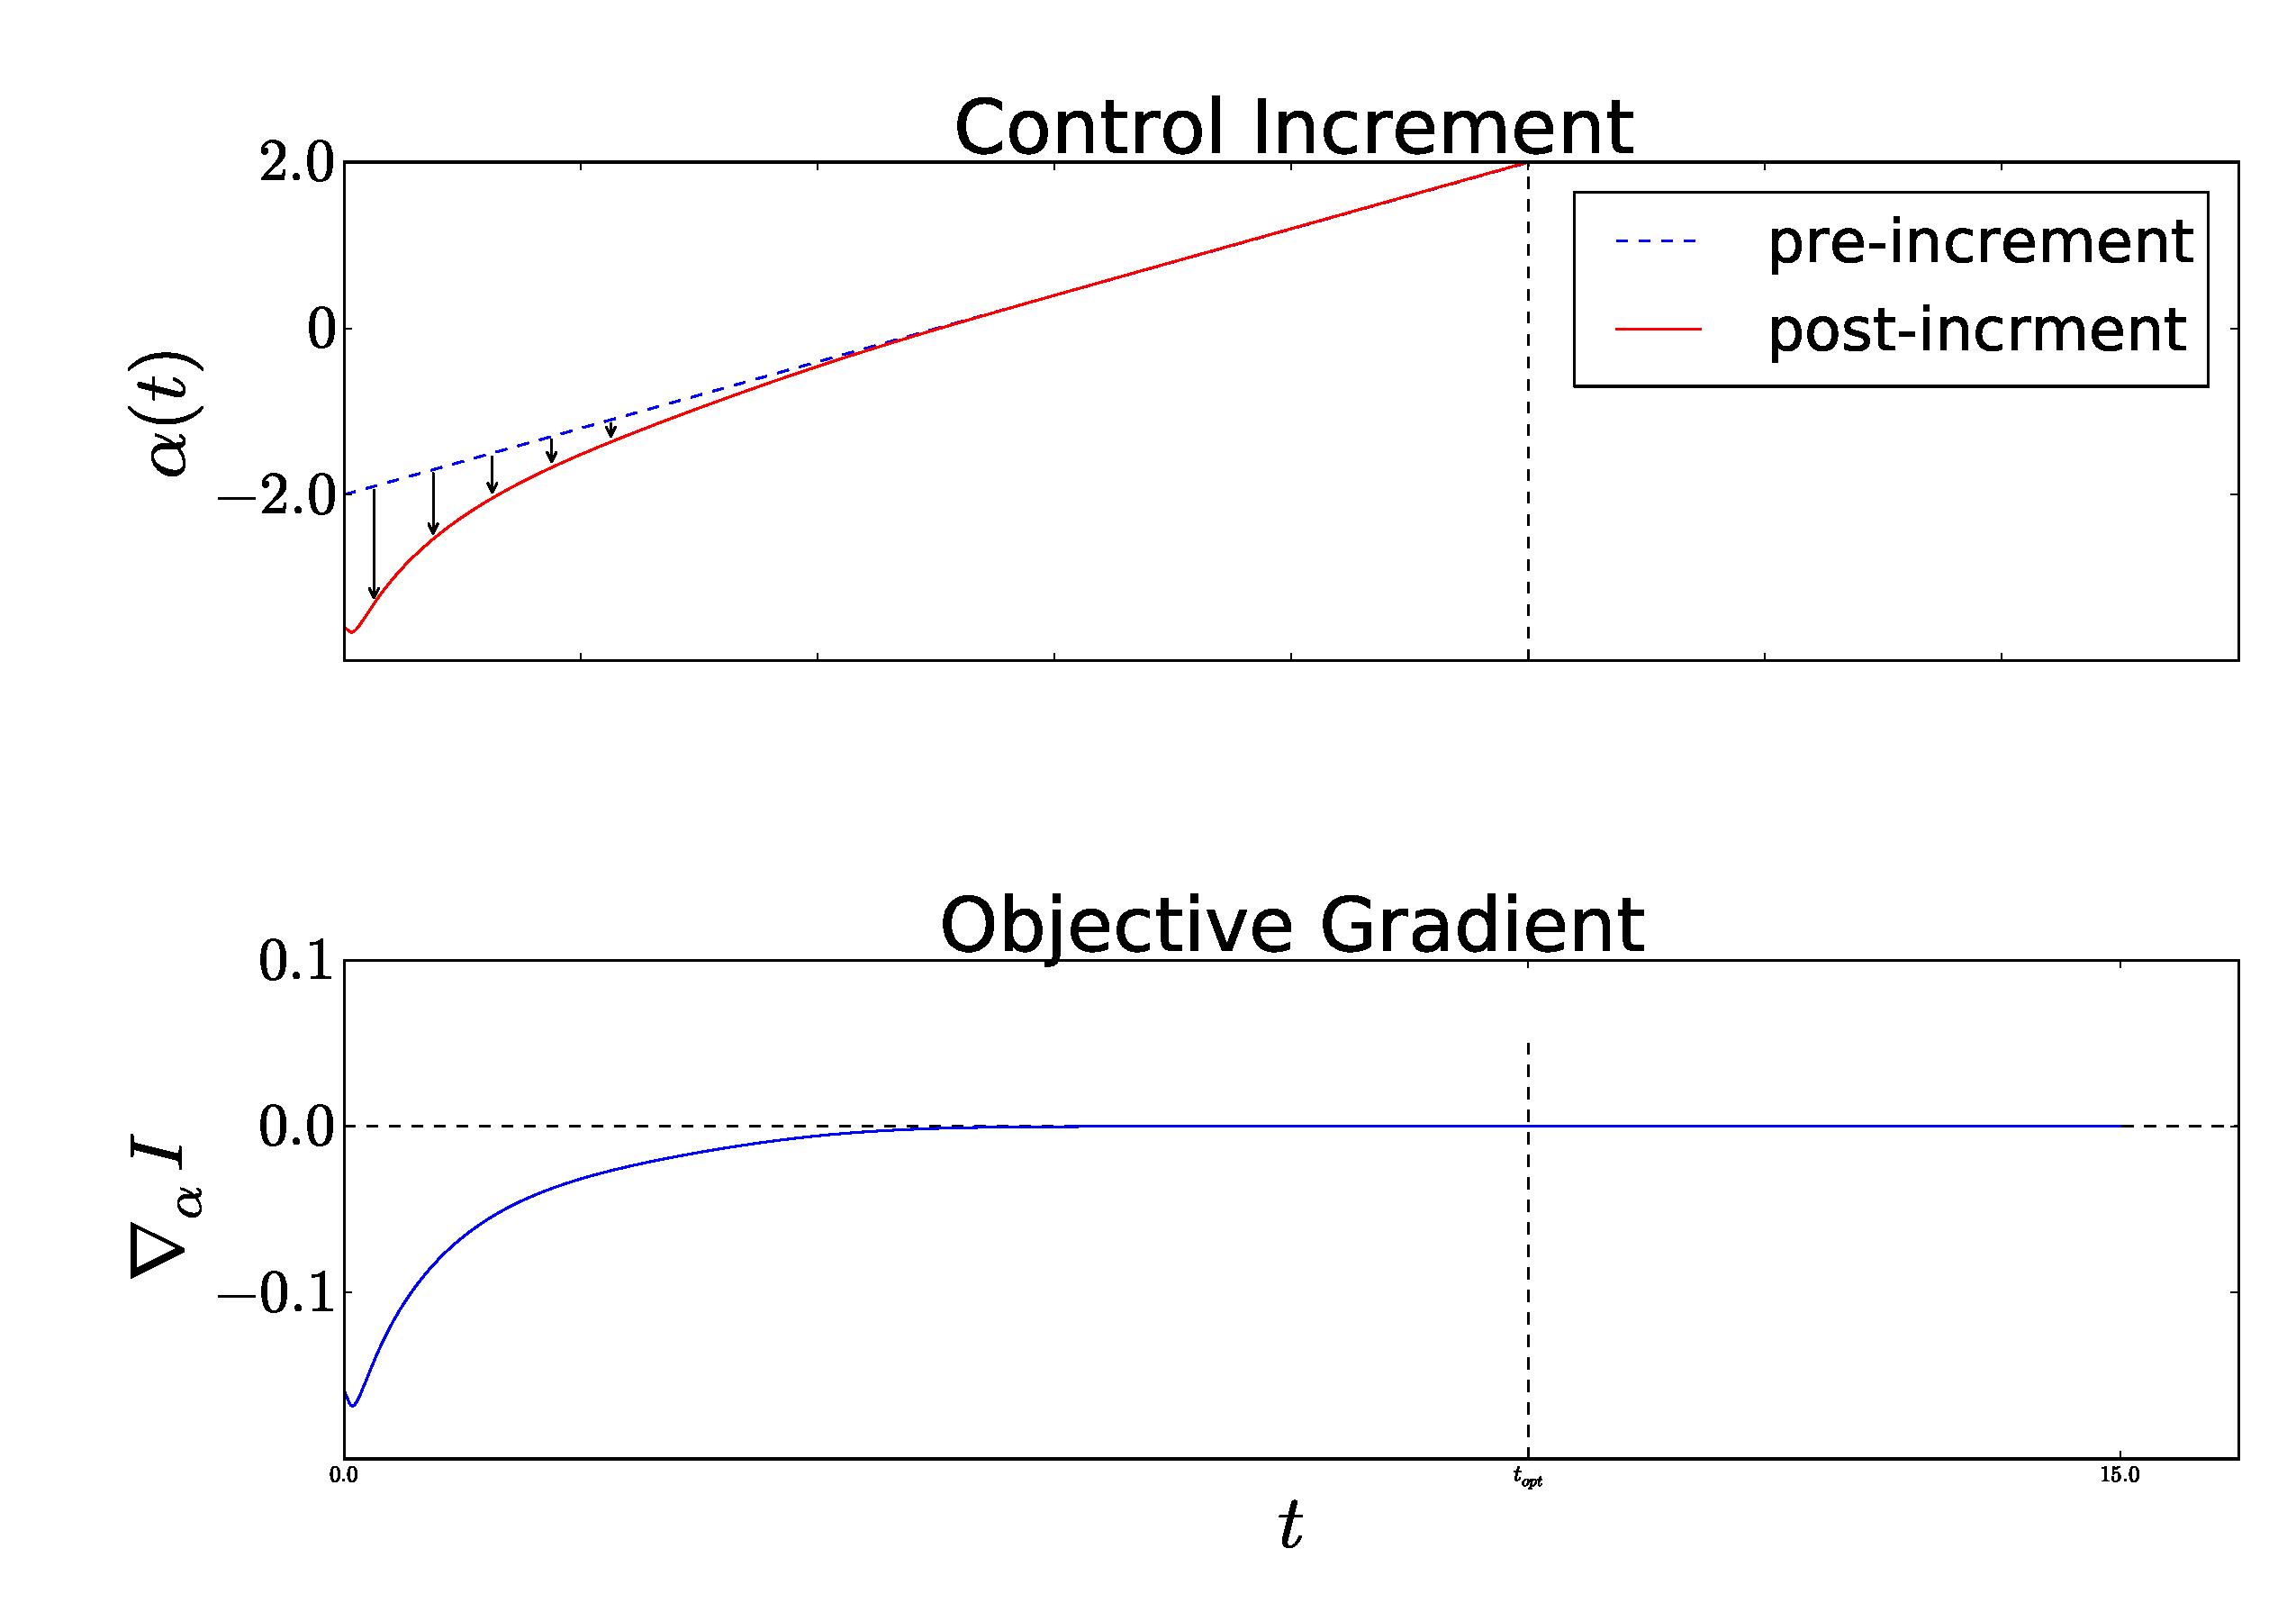
\includegraphics[width=\textwidth]{Figs/FP_Adjoint/control_increment_example.pdf}
  \caption[Single control Increment Illustration]{Illustration of how the
  control is incremented given the gradient. In the top panel, we show the
  initial control in dashed and the incremented control in solid with arrows
  indicating the incremental change. In the bottom panel, we visualize the
  corresponding value of $\delta I/ \delta \a (t)$. }
  \label{fig:example_control_increment}    
\end{center}
\end{figure}   
           
\begin{figure}[htp] 
\begin{center}
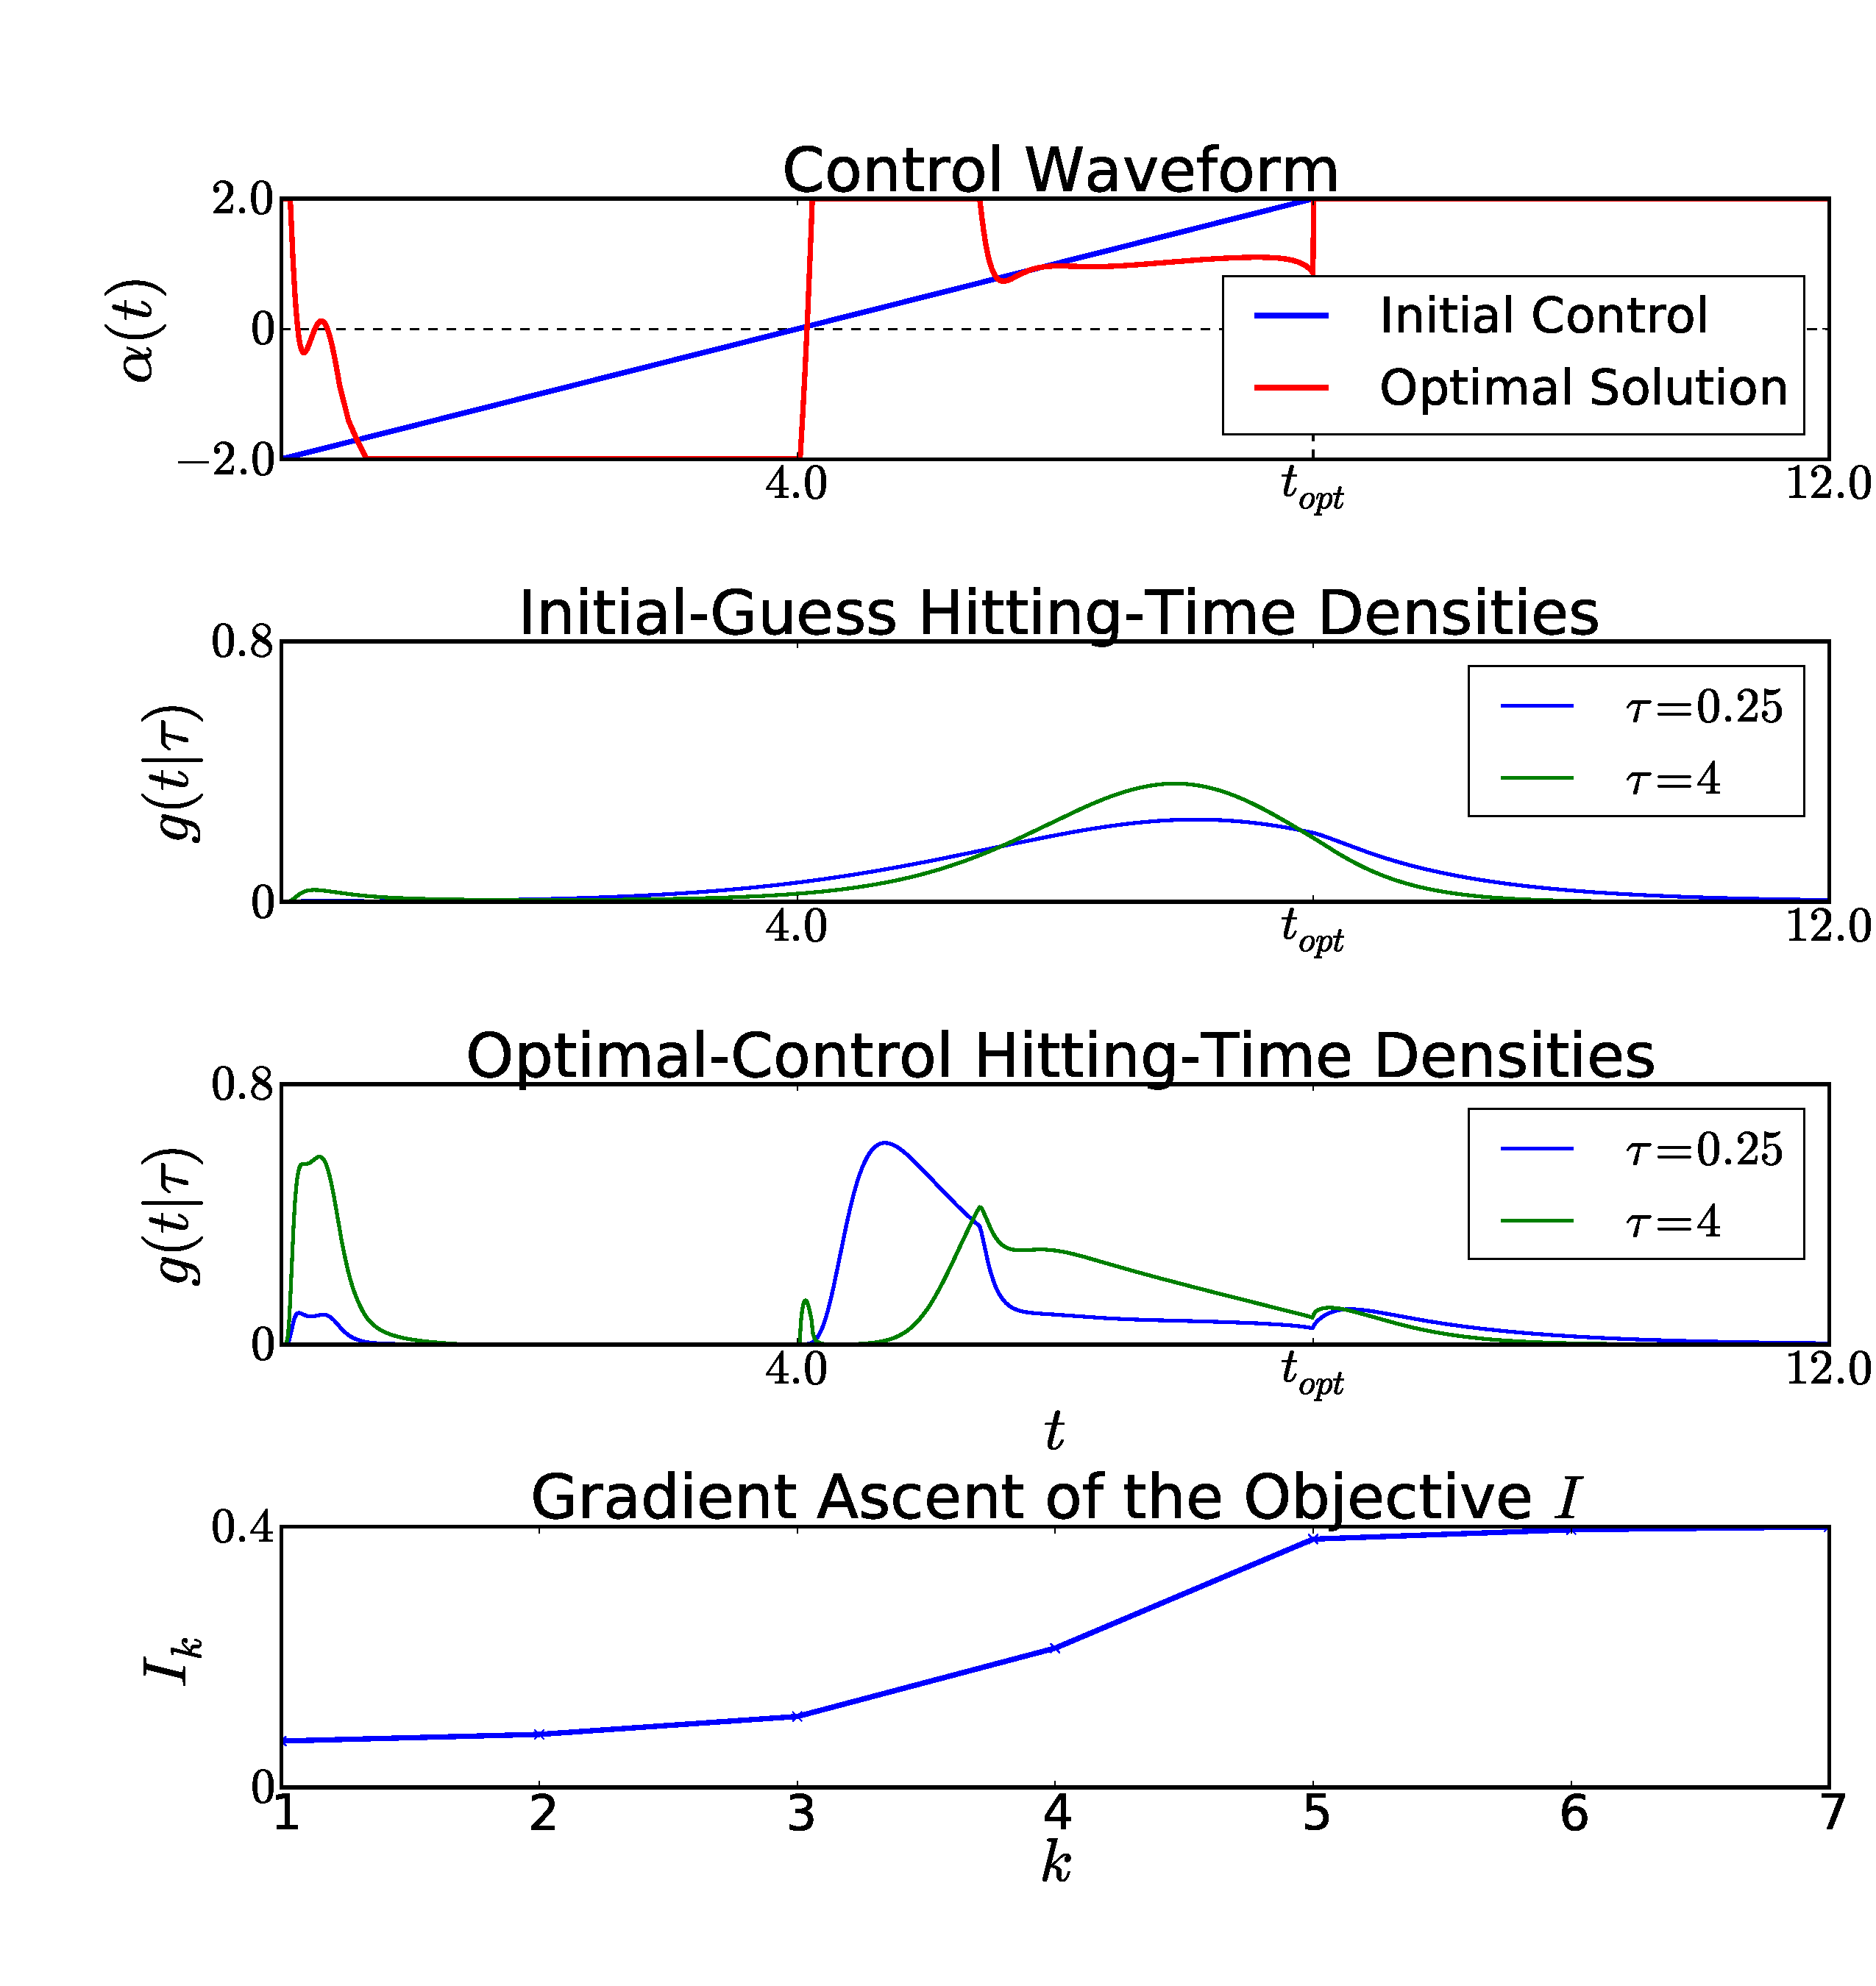
\includegraphics[width=1\textwidth]{Figs/AdjointOptimizer/GradientAscent_Nt2.pdf}
  \caption[Gradient Ascent for the Optimal Stimulation]{Example gradient
  ascent for the optimization of $I$ in
  \cref{eq:I_mutual_info_objective_in_terms_of_dixf} illustrating that the
  effect of the optimal control $\a_{opt}$ is to effectively 'separate' the
  hitting time distributions corresponding to the potential values of $\tc$.
  Top
  panel, the initial and the optimal optimal controls, $\a_{0}(t), \a_{opt}(t)$. Second panel shows the hitting time distributions $g(t|\tc)$ conditional on
  using the initial control, $\a_0$.
  The third panel again shows $g(t|\tc)$, but this time conditional on the
  optimal, $\a_{opt}$.
 The bottom panel shows the progress of the Objective Mutual Information ($I$) 
  (\cref{eq:J_mutual_info_objective}) as a function of the gradient ascent
  iterations (here the algorithm converged in 9 iterations). It is clear that
  th optimal control significantly improves the objective in comparison to the
  initial guess.}
  \label{fig:example_gradient_ascent}   
\end{center}   
\end{figure}    
 
In \cref{fig:example_gradient_ascent}, we get an intuitive 
feeling for what the 'optimal control' is attempting to do - it tries to
'pull apart' the hitting time distributions, such that an observed hitting time
can most cleanly be attributed to one of the potential parameter values, $\t$.
For the combination of known parameters, $\m, \s$ and prior $\rho$, used in
\cref{fig:example_gradient_ascent}, the optimal control first suppresses firing
for an initial time-segment and then maximally stimulates firing in the
remaining time. 
It is visually obvious that the result on $g(t|\tc)$ is to go
from a case where the two possible, hitting time distributions lie on top of each other, to one where they are clearly
delineated. Thus given an observation from the optimally stimulated system, one
would be able to much more confidently estimate what was the underlying value of
$\tau$ that produced the observation. 

\subsection{Switch point sweep}
Given the optimal solution obtained in \cref{sec:gradient_ascent}, we suspect
that the optimal solution is bang-bang, in the sense of 'hold  everything back
and then excite maximally'. It is interesting to check how sensitive the
objective is to the exact value of the switching time, $t_{switch}$. If it is
not very sensitive, it would be practically useful as the exact
optimization of the PDE-based optimization will not be
necessary, and any 'bang-bang' solution will achieve satisfactory improvement in
estimation. 

Therfore, we sweep through the switch point of exactly when the
bang-bang switch occurs and see how it impacts the resulting objective, $I$.
The results are in \cref{fig:sweep_switchtime}. It seems that, at least for this
parameter set, there is an improvement in the objective by putting the switching
point past $t=6$, but going much beyond that there is no real difference. 

\begin{figure}[htp]
\begin{center}
  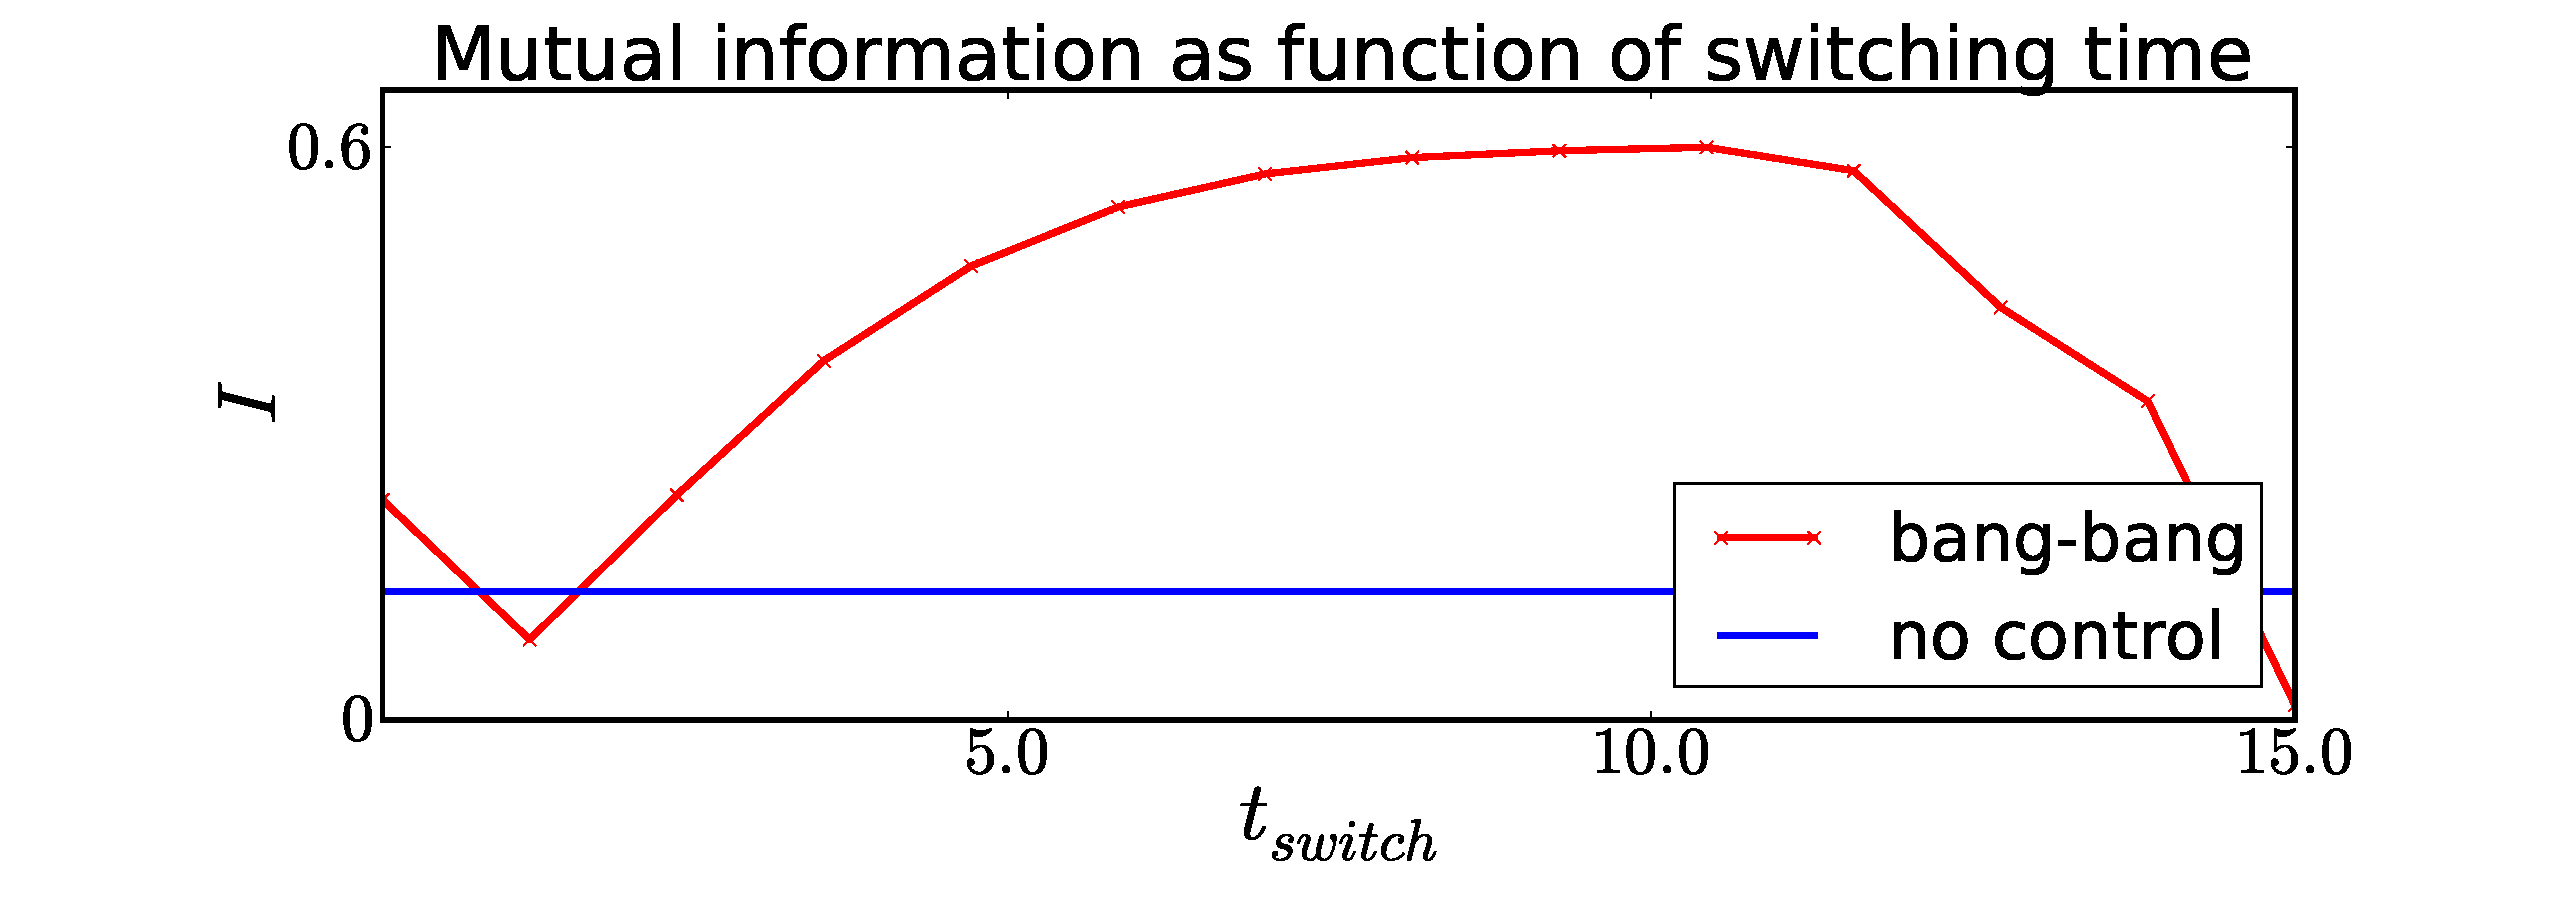
\includegraphics[width=1\textwidth]{Figs/AdjointOptimizer/SweepSwitchpoint_wide.pdf}
  \caption[Effect of Switching time on Mutual Info Objective]{Effect of
  Switching time on Mutual Info Objective. Plotted is the objective, $I$, as a
  function of the switching time, $t_{switch}$, of a bang-bang switching control
  as in the top panel of \cref{fig:example_gradient_ascent}. The same
  simulation parameters are used as in \cref{fig:example_gradient_ascent}. The
  red line is the value of $I$ as function of a switching time, $t_{switch}$
  between maximally-inhibitive to maximally-excitatory control (a bang-bang
  control). The blue line, plotted for refernce, is the value of
  $I$ for no control ($\a=0, \forall t$))}
  \label{fig:sweep_switchtime}
\end{center}
\end{figure}


\subsection{Optimization Method Sensitivity to Problem Parameters}
We explore the effect of the number of points
$\t_i$ in the prior and the dispersion in the prior; the initial
guess for $\a(\cdot)$ and the values of the known parameters $\m, \s$. 

\subsubsection{Number of Points, higher moments of the prior}
We wonder whether the exact shape of the prior matter or whether the first two
moments (mean, variance) are sufficient to determine the optimal control. We
make a simple experiment where we compute the optimal control as in
\cref{sec:gradient_ascent} for two very similar priors, the first using 2 points
in the prior and in the second using 3 points, but both priors have the same
log-mean and log-variance. See \cref{fig:prior_shape_impact}. We observe that
the optimal control is essentially the same. This suggests that for practical
purposes it suffices to make the optimization with a 2-point prior that matches
the (log-) variance of the more detailed prior distribution.
 
%\usepackage{graphics} is needed for \includegraphics
\begin{figure}[htp]
\begin{center}
  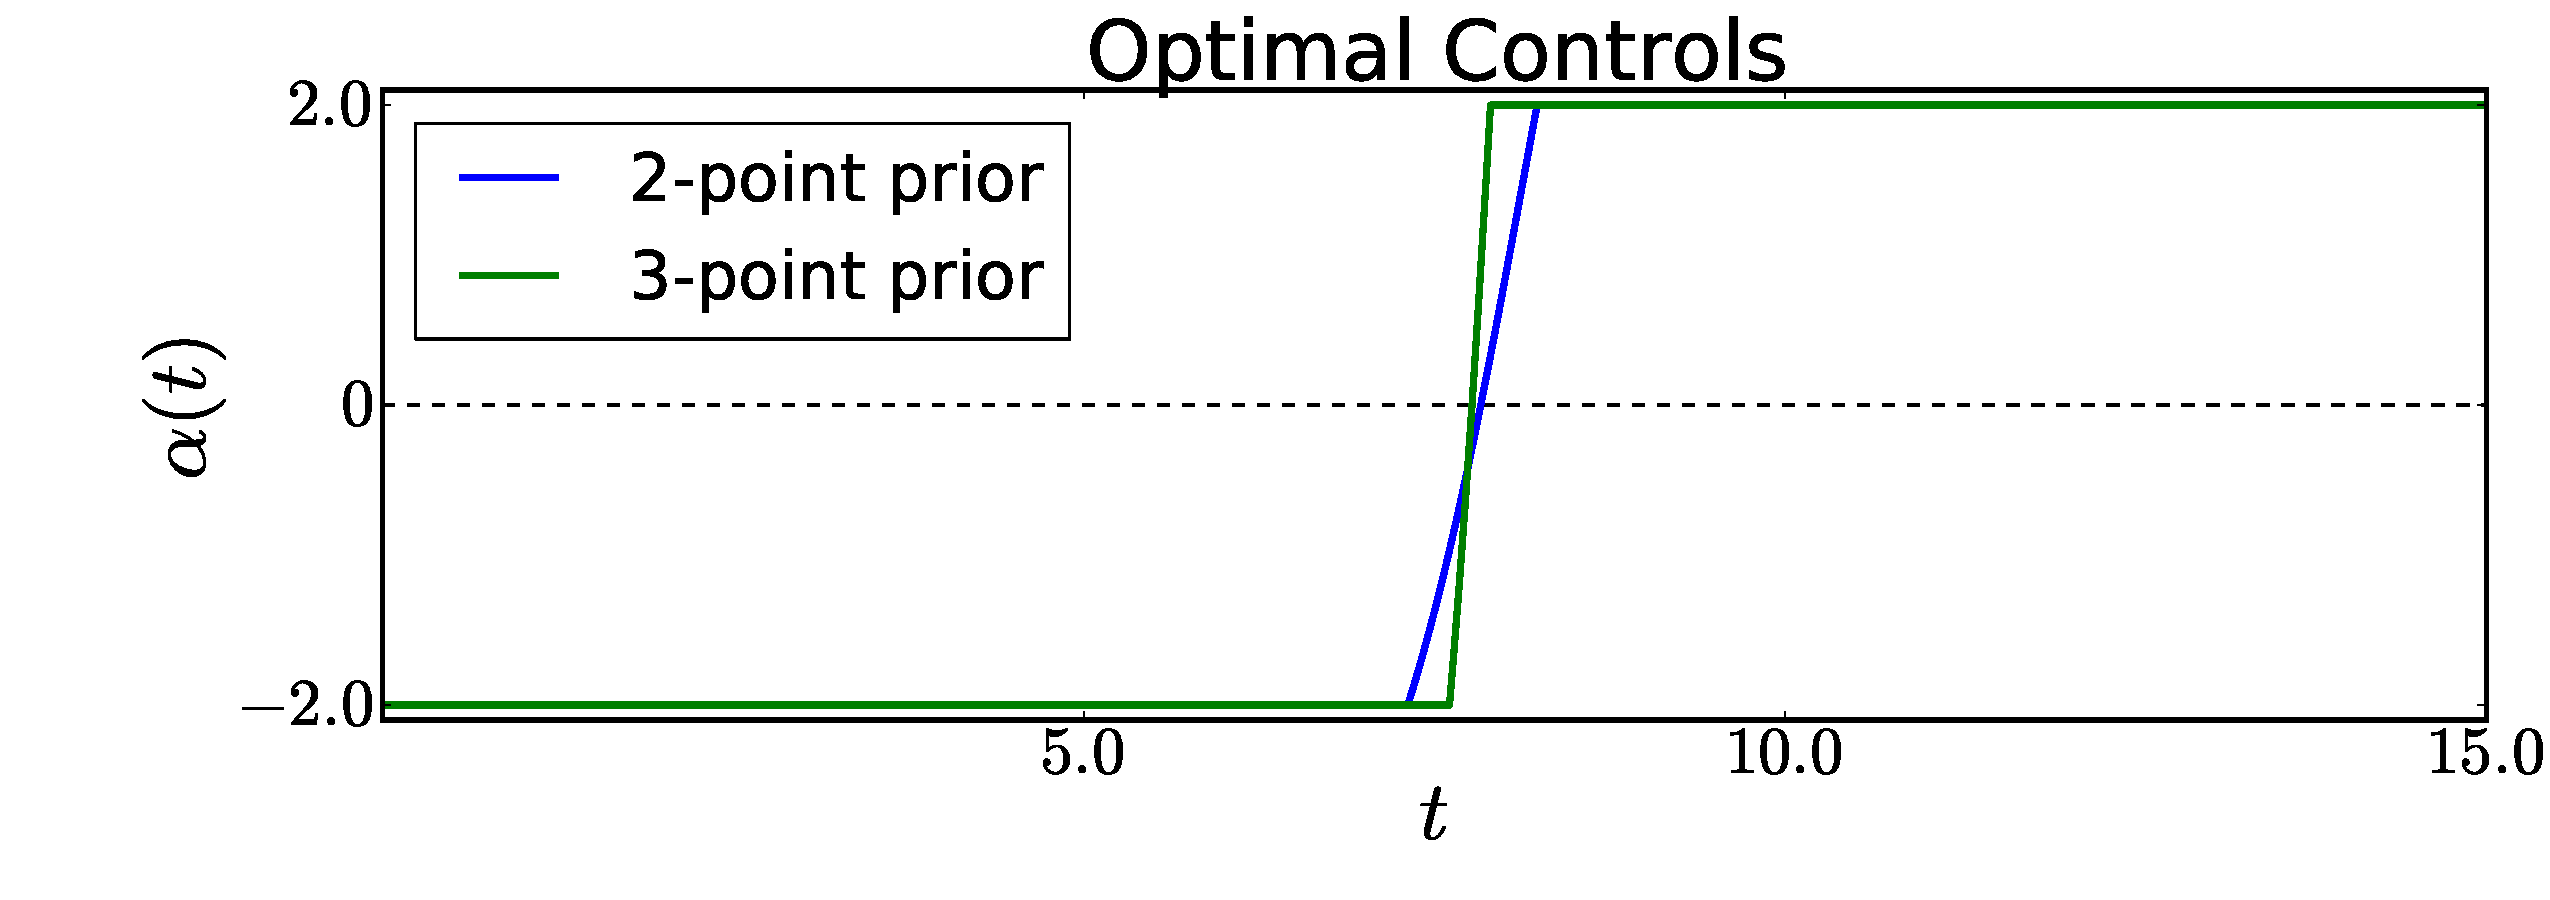
\includegraphics[width=1\textwidth]{Figs/AdjointOptimizer/NumberOfTausEffect.pdf}
  \caption[Detailed-Shape-of-Prior Impact]{Effect of detailed shape of the prior
  on the Optimal Control.} 
  \label{fig:prior_shape_impact} 
\end{center}
\end{figure}

\subsubsection{The dispersion of the prior}
We wonder whether the dispersion of the prior, quantified by the ($log$-)
variance changes the optimal control. Again, we take two 2-point priors, one with
particles at $\tc = [.25, 4]$ and the other at $\tc = [.75,1.3]$, the results
are shown in \cref{fig:prior_dispersion_impact}. It is clear that while the
general shape of the optimal control is the same, regardless of the 'width' of
hte prior, there is some difference. We further investigate the
practical difference between the two priors in the section on estimation,
\cref{sec:batch_estimation}.

%\usepackage{graphics} is needed for \includegraphics
\begin{figure}[htp]
\begin{center}
  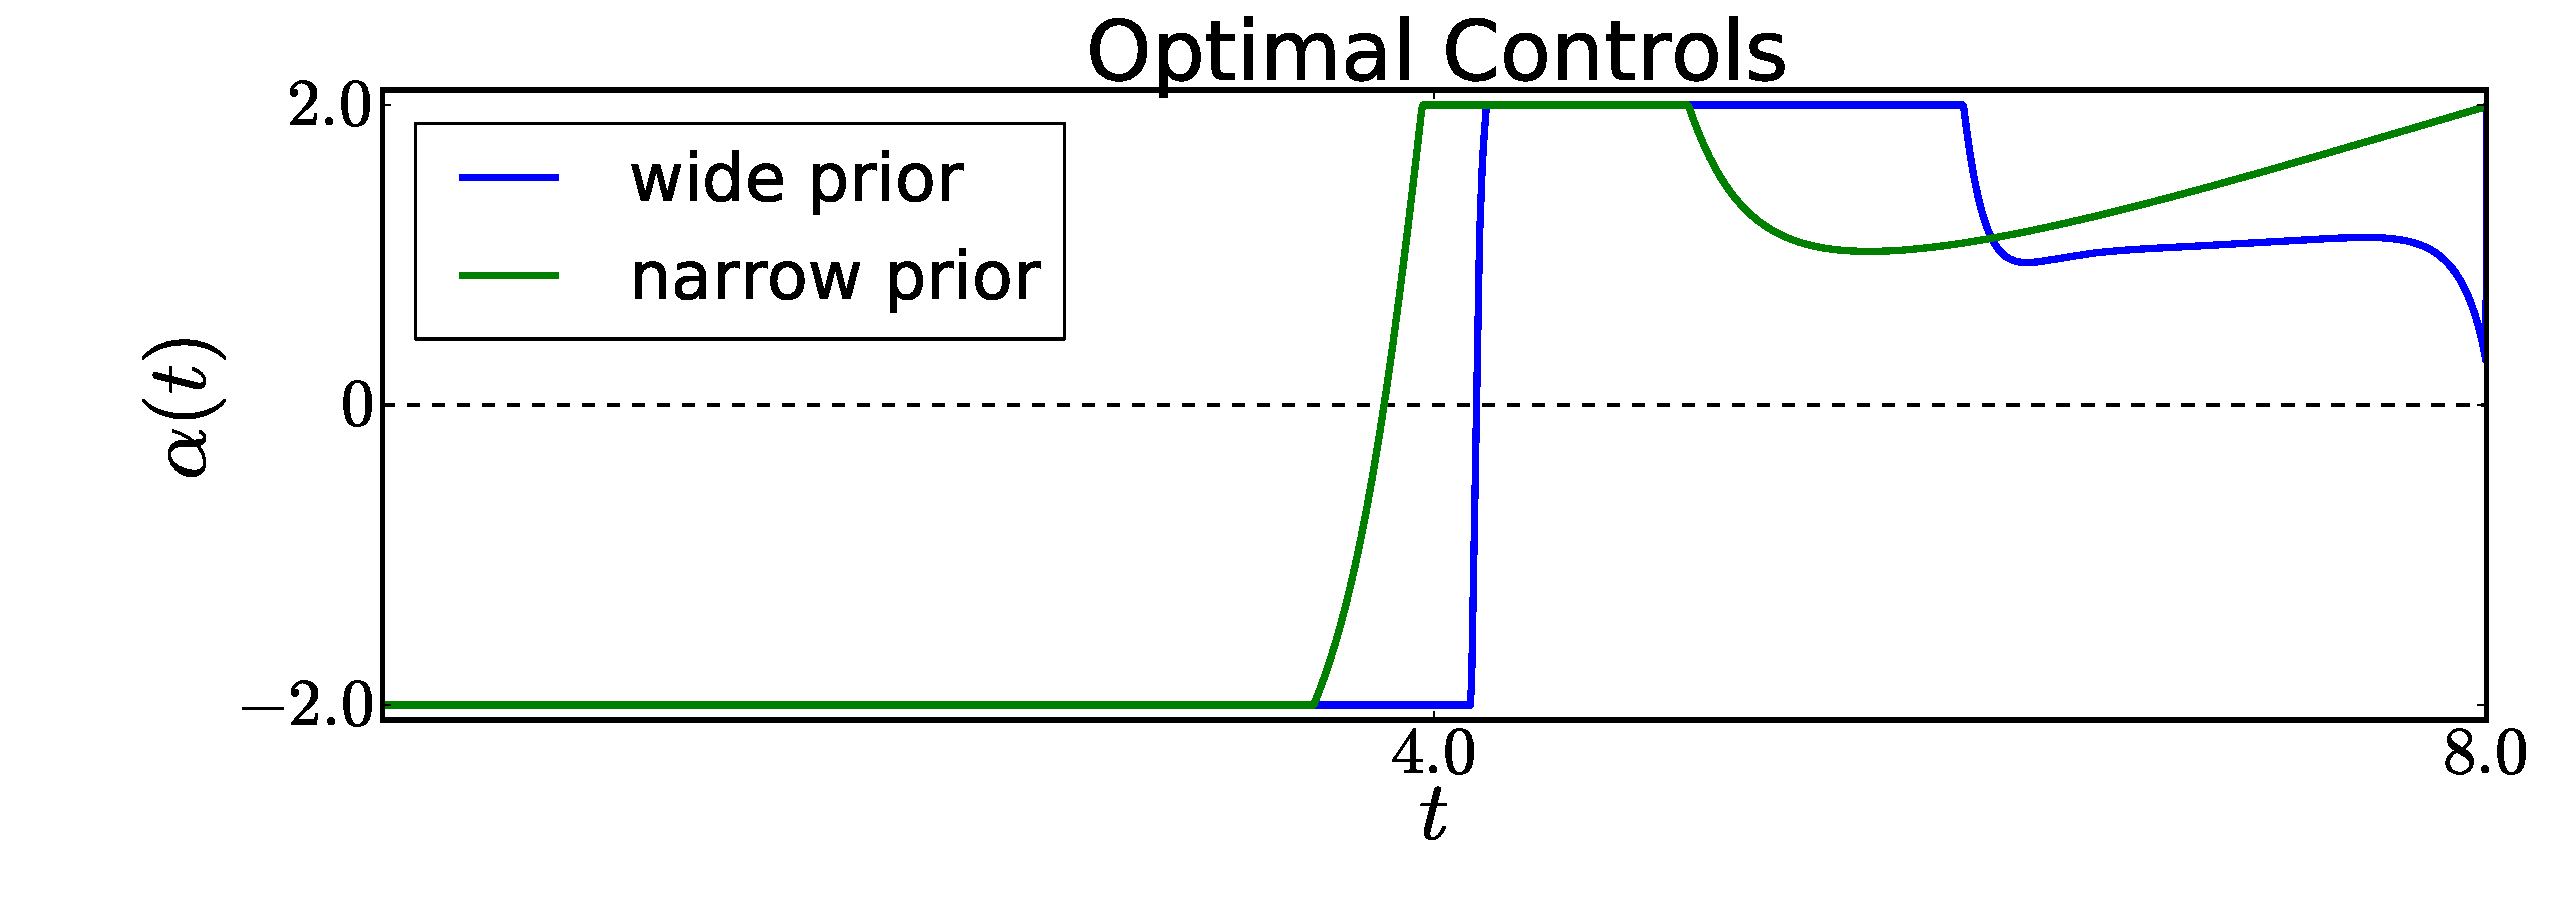
\includegraphics[width=\textwidth]{Figs/AdjointOptimizer/PriorSpread.pdf}
  \caption[Variance-of-Prior Effect]{Effect of variance-of-prior on
  optimal stimulation. For the 'wide prior', we set the simple, uniform 2-point prior at
   $\tc =  [0.25, 4]$, while for the 'narrow prior', they are positioned much
   closer to each other at $\tc =   [0.75, 1/.75 ]$  }
  \label{fig:prior_dispersion_impact} 
\end{center}
\end{figure}

\subsubsection{The initial guess for the control $\a_0$}
Like all gradient-based optimization procedures, ours is sensitive to the choice
of initial guess for the independent variable, i.e.\ the choice of $\a_0$. 

It turns out that indeed the choice of $\a_0$ has a strong influence on what the
scheme finds as optimal. We illustrate this in \cref{fig:ICs_for_control}. We
proceed as follows, for three different priors, a wide, medium and concentrated
one, we run the optimization scheme from four different initial guesses for
$a_0$ - 
\begin{enumerate}
\item zero for the entire (optimization) time-interval
\item linearly increasing from the lower to the upper control bound over the
optimization interval
\item a sinusoidal wave from max to min and again to max
\item max for the entire optimization time-interval 
\end{enumerate}
In \cref{fig:ICs_for_control}, we see that for different initial guesses the
optimization routine finds different optimal controls. It seems that it is
easier to find a good optimal control for the wide prior and more difficult for
the concentrated prior in which case, the optimizer cannot improve on the
objective except if started with the 'sinusoidal' initial guess.

\begin{figure}[h]
\begin{center}  
\subfloat[Wide Prior]
{
\label{fig:wide_prior_opt_ics}
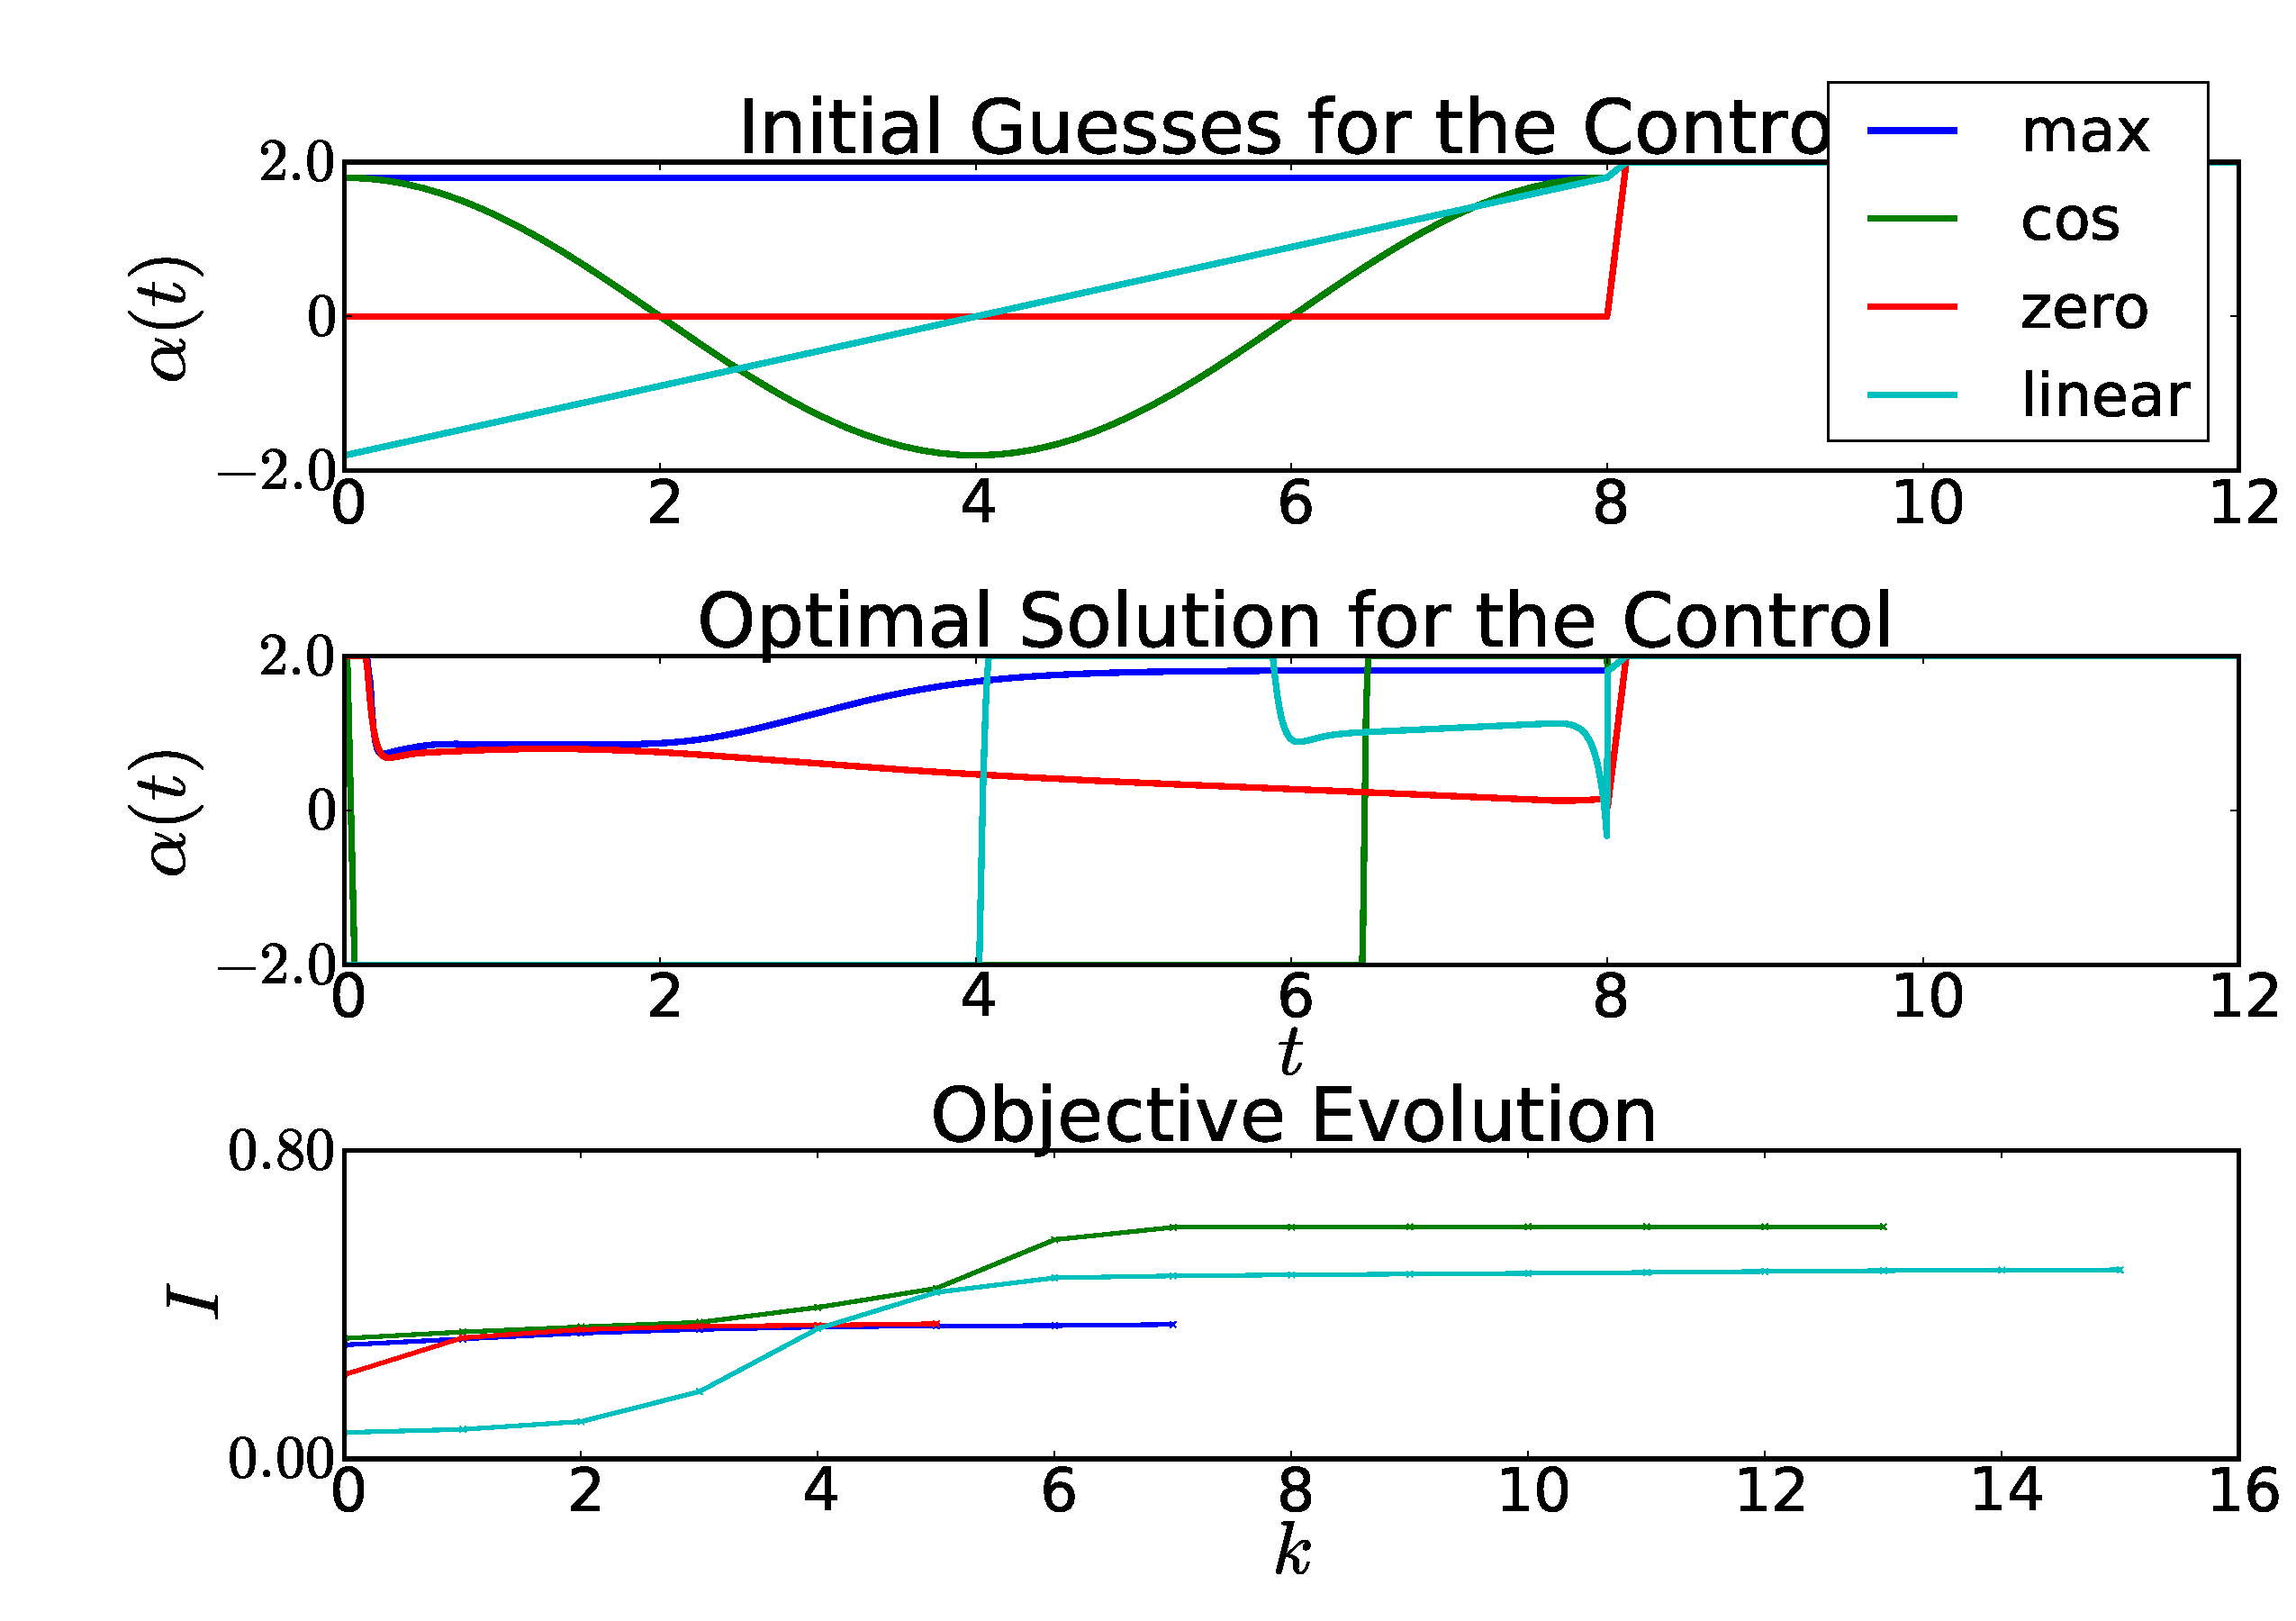
\includegraphics[width=0.5\textwidth]
{Figs/AdjointOptimizer/OptimizerICswide_prior.pdf}
}
\subfloat[Medium Prior] 
{
\label{fig:medium_prior_opt_ics}
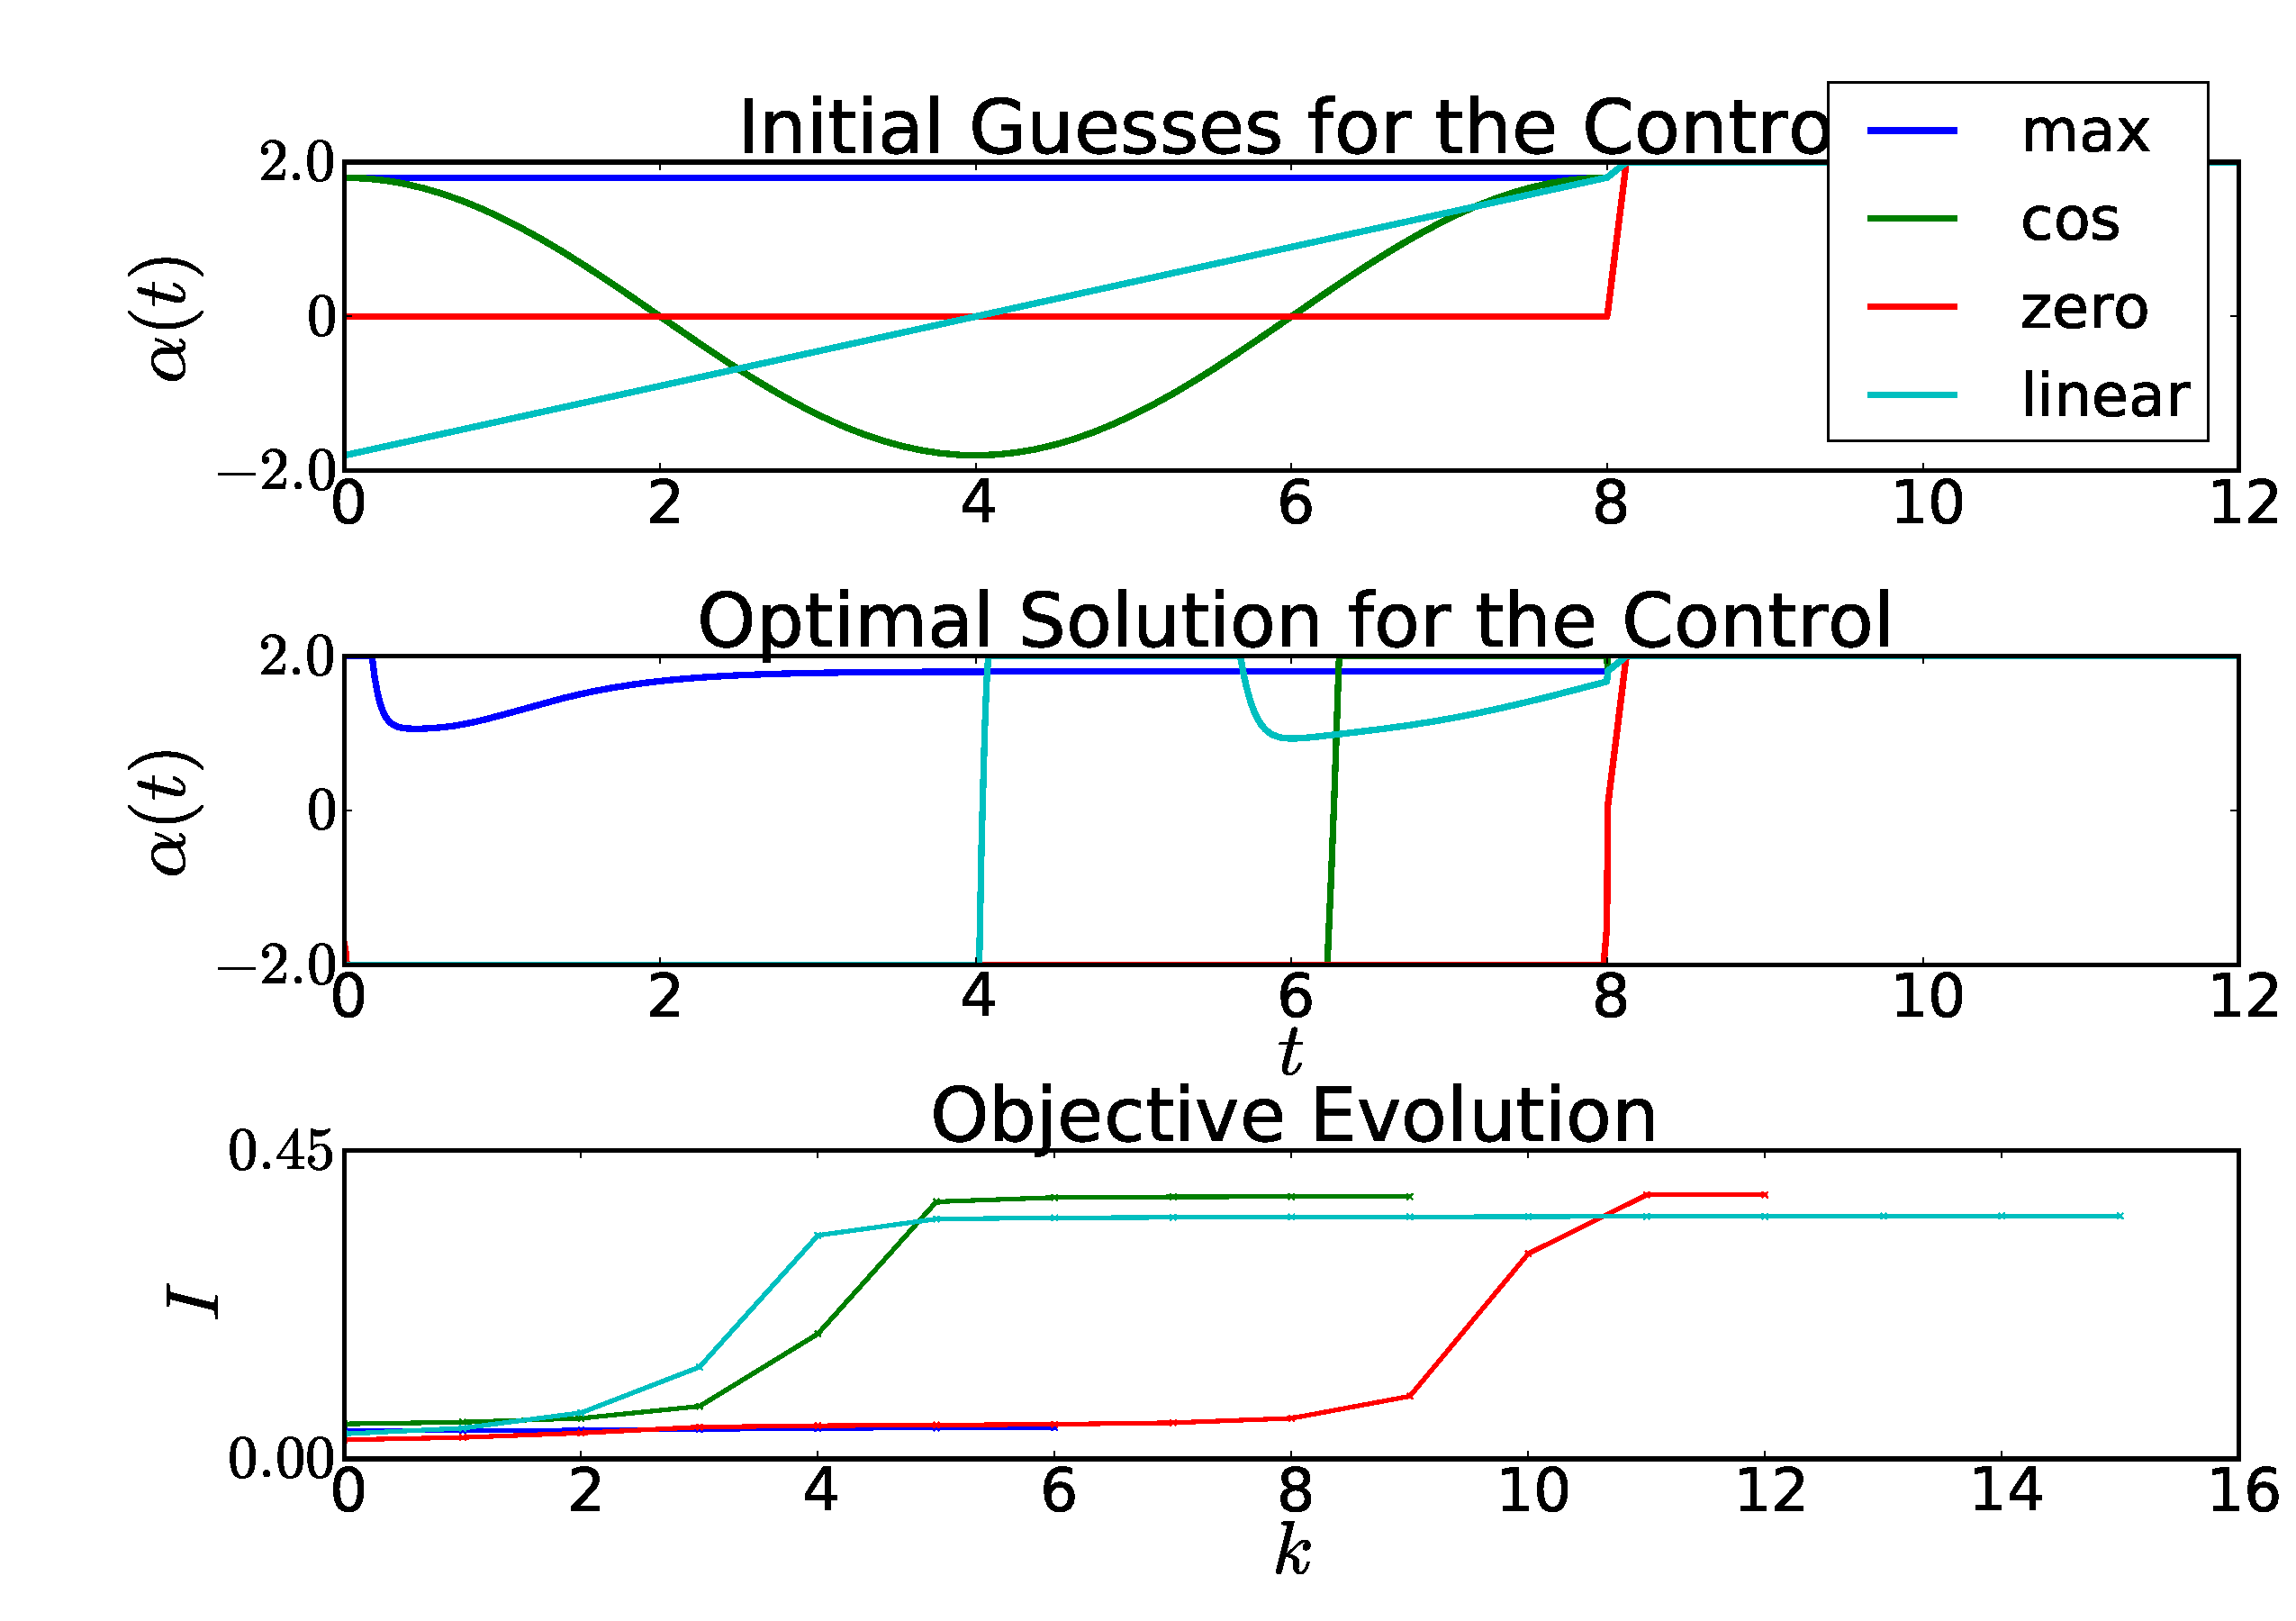
\includegraphics[width=0.5\textwidth]
{Figs/AdjointOptimizer/OptimizerICsmedium_prior.pdf}
}
\\
\subfloat[Concentrated Prior]  
{
\label{fig:medium_prior_opt_ics}
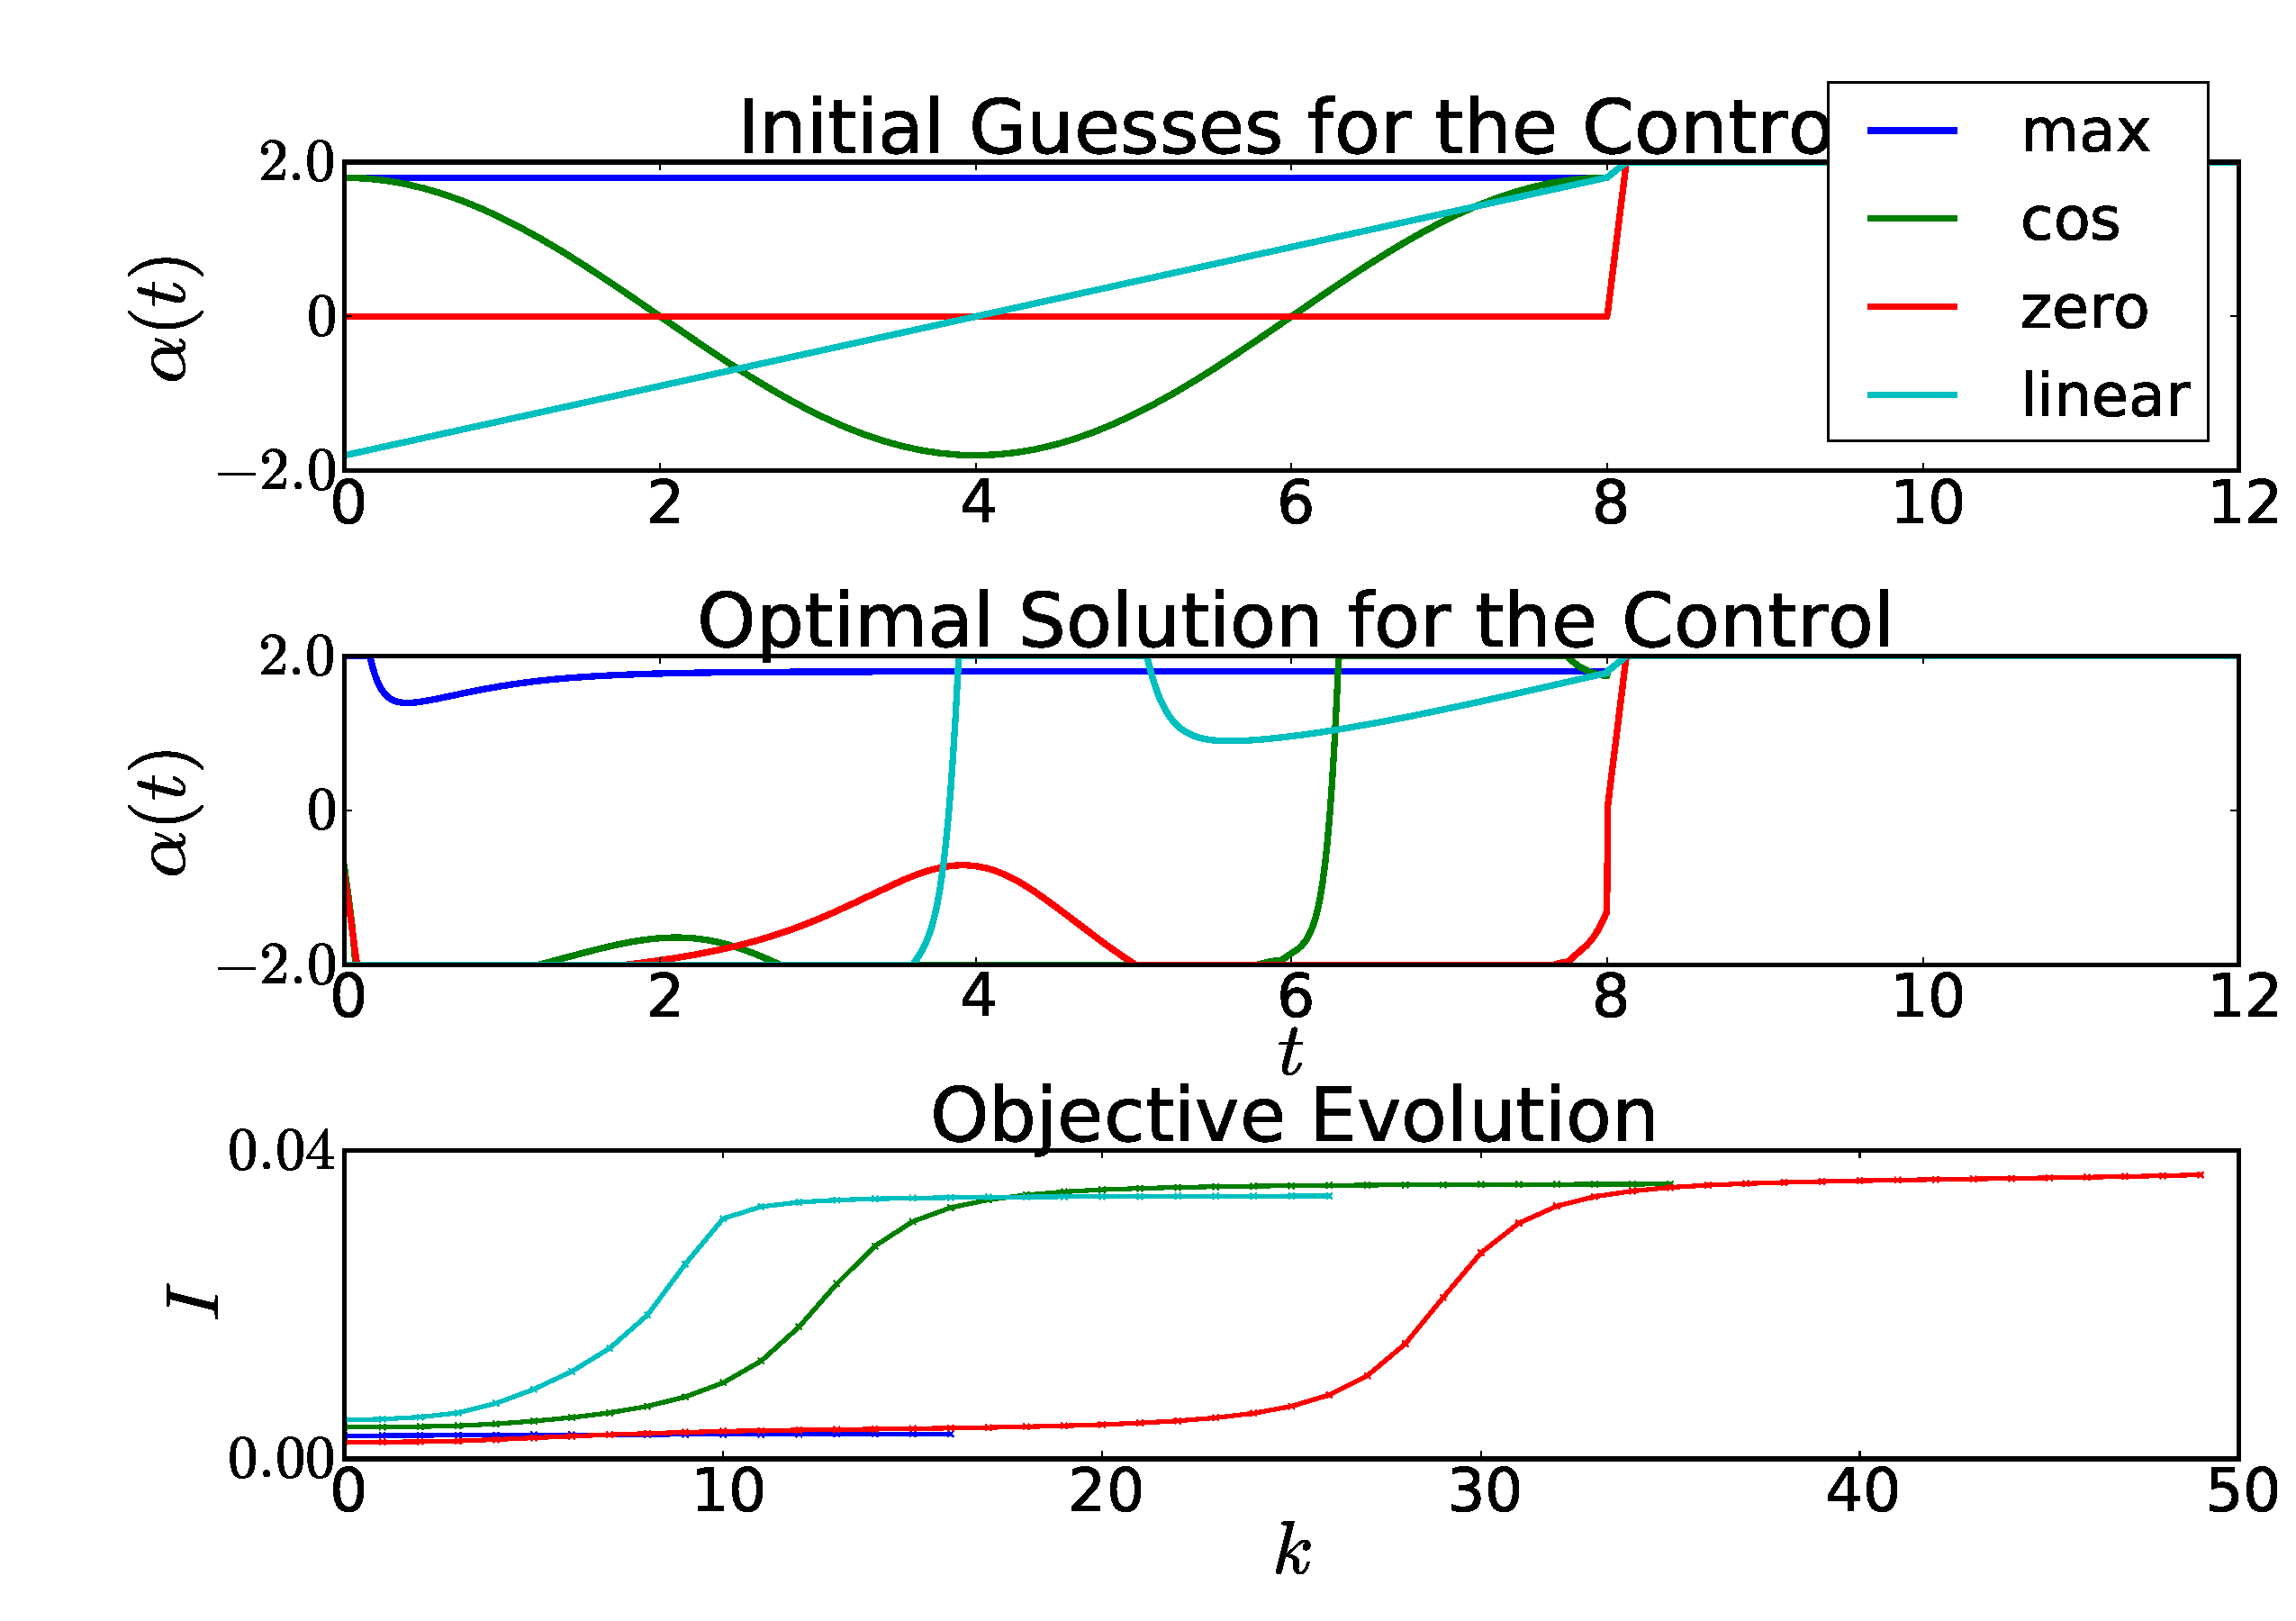
\includegraphics[width=0.5\textwidth]
{Figs/AdjointOptimizer/OptimizerICsconcentrated_prior.pdf}
}
\caption[Dependence on initial guess for control]{Illustrating the dependence
of the optimization scheme on the initial guess for the optimal control. 
On the top panel of each sub-float we have the initial guess, in the middle
panel we show the corresponding solution obtained by the optimization routine;
in the bottom panel we show the corresponding evolution of the objective. Note
that the general shape of the optimal control depends more on the IC then the
spread of the prior distribution of $\tc$.}
\label{fig:ICs_for_control}
\end{center}
\end{figure}

\subsubsection{The value of the known parameters $\mu, \s$}
So far we have restricted ourselves to a base-case scenario of the assumed known
parameters, $\mu, \s$. We now redo the basic analysis by varying these.

We look at 6 qualitatively different parameter values, in
\cref{tab:mu_sigma_perturbation}.
\begin{centering} 
\begin{table}
\begin{tabular}{cccc}
Regime meaning & $\m$ & $ \s$ & Meaningful Objective Improvement?\\ \hline
 Negative $\m$ & -0.5& 1 & YES\\ 
 Small-perturbation $\m$ &0.1&1   & YES\\ 
 Very-Positive $\m$ & 1&1  & YES\\
    Smaller $\s$ &                 0&0.3 & YES\\ 
 Small-perturbation $\s$  &        0&0.9 & YES\\ 
                Larger $\s$ &      0&1.5 & YES\\ 
\end{tabular}
\caption{TODO: This table is just for internal consumption - what is the best
way to present this table?

Perturbation parameter values and a YES/NO as to whether the
optimization routine can find significant improvements in the
objective, recall that small-perturbations, mean small relative to
the base case $\m, \s=0,1$.
All examples use the same, 2-pt, prior, $\tc = 
[0.5, 2]$}
\label{tab:mu_sigma_perturbation}
\end{table}
\end{centering}

Unfortunately, while for small perturbation, lines 2,5 in
\cref{tab:mu_sigma_perturbation}, the results are the same as for the base-case,
$\m,\s = 0,1$, for the more significant perturbations, the iterative
 optimization method is not able to progress to significantly better objective
 values and the ascent terminates after only one or two iterations. Clearly some 
improvement can be made here.

\clearpage

\section{Batch Estimation}
\label{sec:batch_estimation}
We now proceed to generate a large sample of hitting times with several type
of controlled stimulation and then estimate the unknown
parameter after observing the whole sample. We call this 'batch' estimation as opposed to
'online' estimation where estimates are updated after every single observation
and the control is also updated according to the updated prior distribution.
Online estimation is performed in the next
section, \cref{sec:online_estimation}).

We assume that the true parameters governing \cref{eq:X_evolution_uo_control} are
$$ \m = 0; \tc = 1; \s = 1;
$$ We will assume we know $\s, \m$ and do not know the time constant, $\tc$ so
we are trying to maximize the Mutual Information between the random hitting
time, $\ts$, and $\tc$. In the parlance of the neuroscience literature this
parameter set corresponds to what is known as the 'Sub-Threshold, High-Noise'
regime, \cite{Iolov2013}, as long as the control, $\a$ equals zero. Of course,
changing the control sufficiently will move it into the qualitatively different,
'Super-Threshold' regime, which is the case when the process can hit the
threshold even in the absence of noise (in the 'Sub-Threshold' regime, a
non-zero noise parameter is required if any hitting-times are to occur.)

For obtaining the MI-optimal stimulation, we will take a uniform prior on
$\tc$, using 10 $\tc_i$ uniformly spaced in the interval $[0.25, 4.0]$, i.e.
each of the $\tc_i$ in the prior has 1/10. Note that neither the mean nor the
log-mean of the prior correspond to the unknown true, $\tc$ or $\log(\tc)$.
 
The control obtained thus will be tagged as 'opt. In addition we consider the
two optimal control obtained using the 'wide' and 'narrow' 2-point priors as
shown in \cref{fig:prior_dispersion_impact}. We call these 'opt-wide' for the
prior with $\tc =  [0.25, 4]$, and 'opt-narrow' for the prior with  $\tc =  
[0.75, 1/0.75]$.  

In addition, we also use the control where $\a$ is set to the 'critical' value,
$\a = \xth/\tc = 1$, and one where the control is set to its upper
bound, $\a = \amax$.

\subsection{The Estimation Algorithm for the Batch Problem}
We have posed a fairly-simple estimation objective, to estimate $\tau$, which
amounts to single-variable optimization. The negative log-likelihood of an
observed hitting-time set $\{t_n\}$ is
\begin{equation}
l(\tc) = - \sum_n \log ( g(t_n | \tc) ) =  - \sum_n \log \left( -D \di_x f(\xth,
t_n |\tc) \right)
\label{eq:MLE_likelihood}
\end{equation}
We minimize \cref{eq:MLE_likelihood} using the standard single-variable
optimization routine in NumPy based on Brent's method.

% The distributions are exemplified in
% \cref{fig:log_likelihood_beta_examples_100000},
% for three different values of $N_s =  1e5$. We see that for the constant
% stimulations, $\a = \a_{crit}, \a_{max}$ it is very hard to
% distinguish between different values of $\tc$. 
% 
% In \cref{fig:log_likelihood_beta_examples_100000} as well as in 
% \cref{fig:hitting_time_density_g_aopt_bprior}, we get an indication for why
% the 'optimal control' is better than the constants. For the constant control
% the different hitting time densities look like local perturbations of each
% other, either a little more or a little less, but for the optimal control they
% are shifted, which means that we see the first indications that the Opt Control,
% might have some superiority over the 'Crit' Control (for example) as it seems to estimate a $\tc$ closer to 1 (the 'true' value). However, on average, the different shapes of $\a(t)$ seems to have a very limited impact on the estimates for $\tc$ (even though it has a very obvious impact on the shape of the hitting time distribution $g(t)$).

% \begin{figure}[h] 
% \begin{center}
% \subfloat[opt]
% {
% \includegraphics[width=.75\textwidth]
% {Figs/HitTime_MI_TauChar_Adjoint_Estimate/Adjoint_TauChar_Estimator_estimatorWorkbench_b=0x100000_a0.pdf}
% }
% \\
% \subfloat[crit] 
% {
% \includegraphics[width=.75\textwidth]
% {Figs/HitTime_MI_TauChar_Adjoint_Estimate/Adjoint_TauChar_Estimator_estimatorWorkbench_b=0x100000_a1.pdf}
% }
% \\
% \subfloat[max]
% {
% \includegraphics[width=.75\textwidth]
% {Figs/HitTime_MI_TauChar_Adjoint_Estimate/Adjoint_TauChar_Estimator_estimatorWorkbench_b=0x100000_a2.pdf}
% }
% \caption[labelInTOC]{Example of Empirical vs.\ Analytical Hitting time
% distributions, $g(t|\t;\a)$, and the associated log-likelihoods. $N_s = 1e5$
% hits}
% \label{fig:log_likelihood_beta_examples_100000}
% \end{center}
% \end{figure}  
% 
% \clearpage



\subsection{Estimator Comparison}
Recall that we will stimulate the system using 5 stimulation
waveforms.  
\begin{enumerate}
  \item 'opt' - the optimal gradient-ascent-based  control $\a_{opt}$, based on
  a 10-point uniform prior between $[0.25, 4]$
  \item  'opt-wide' - the optimal control using a 2-point prior on  $[0.25, 4]$
  \item 'opt-narrow' - the optimal control using a 2-point prior on $[0.75,
  1/0.75]$
\item   'crit' - the constant control
$\a_{crit}$, ($\a_{crit}(t) =  \xth/\tc$
\item  'max' - the max constant control, $\amax$ ($=2$)
\end{enumerate} 

We now simulate $N_b $ blocks of $N_s$ hitting times each for the
5 alphas and then estimate $\tc$ over each set using MaxLikelihood over our
computed expression for the density, $g(t|\tc; \a(t) )$. 
Naturally, for each control, we use the same Gaussian random draws per block of
$N_s$ hitting of times.

%\usepackage{graphics} is needed for \includegraphics
% \begin{figure}[htp]
% \begin{center}
%   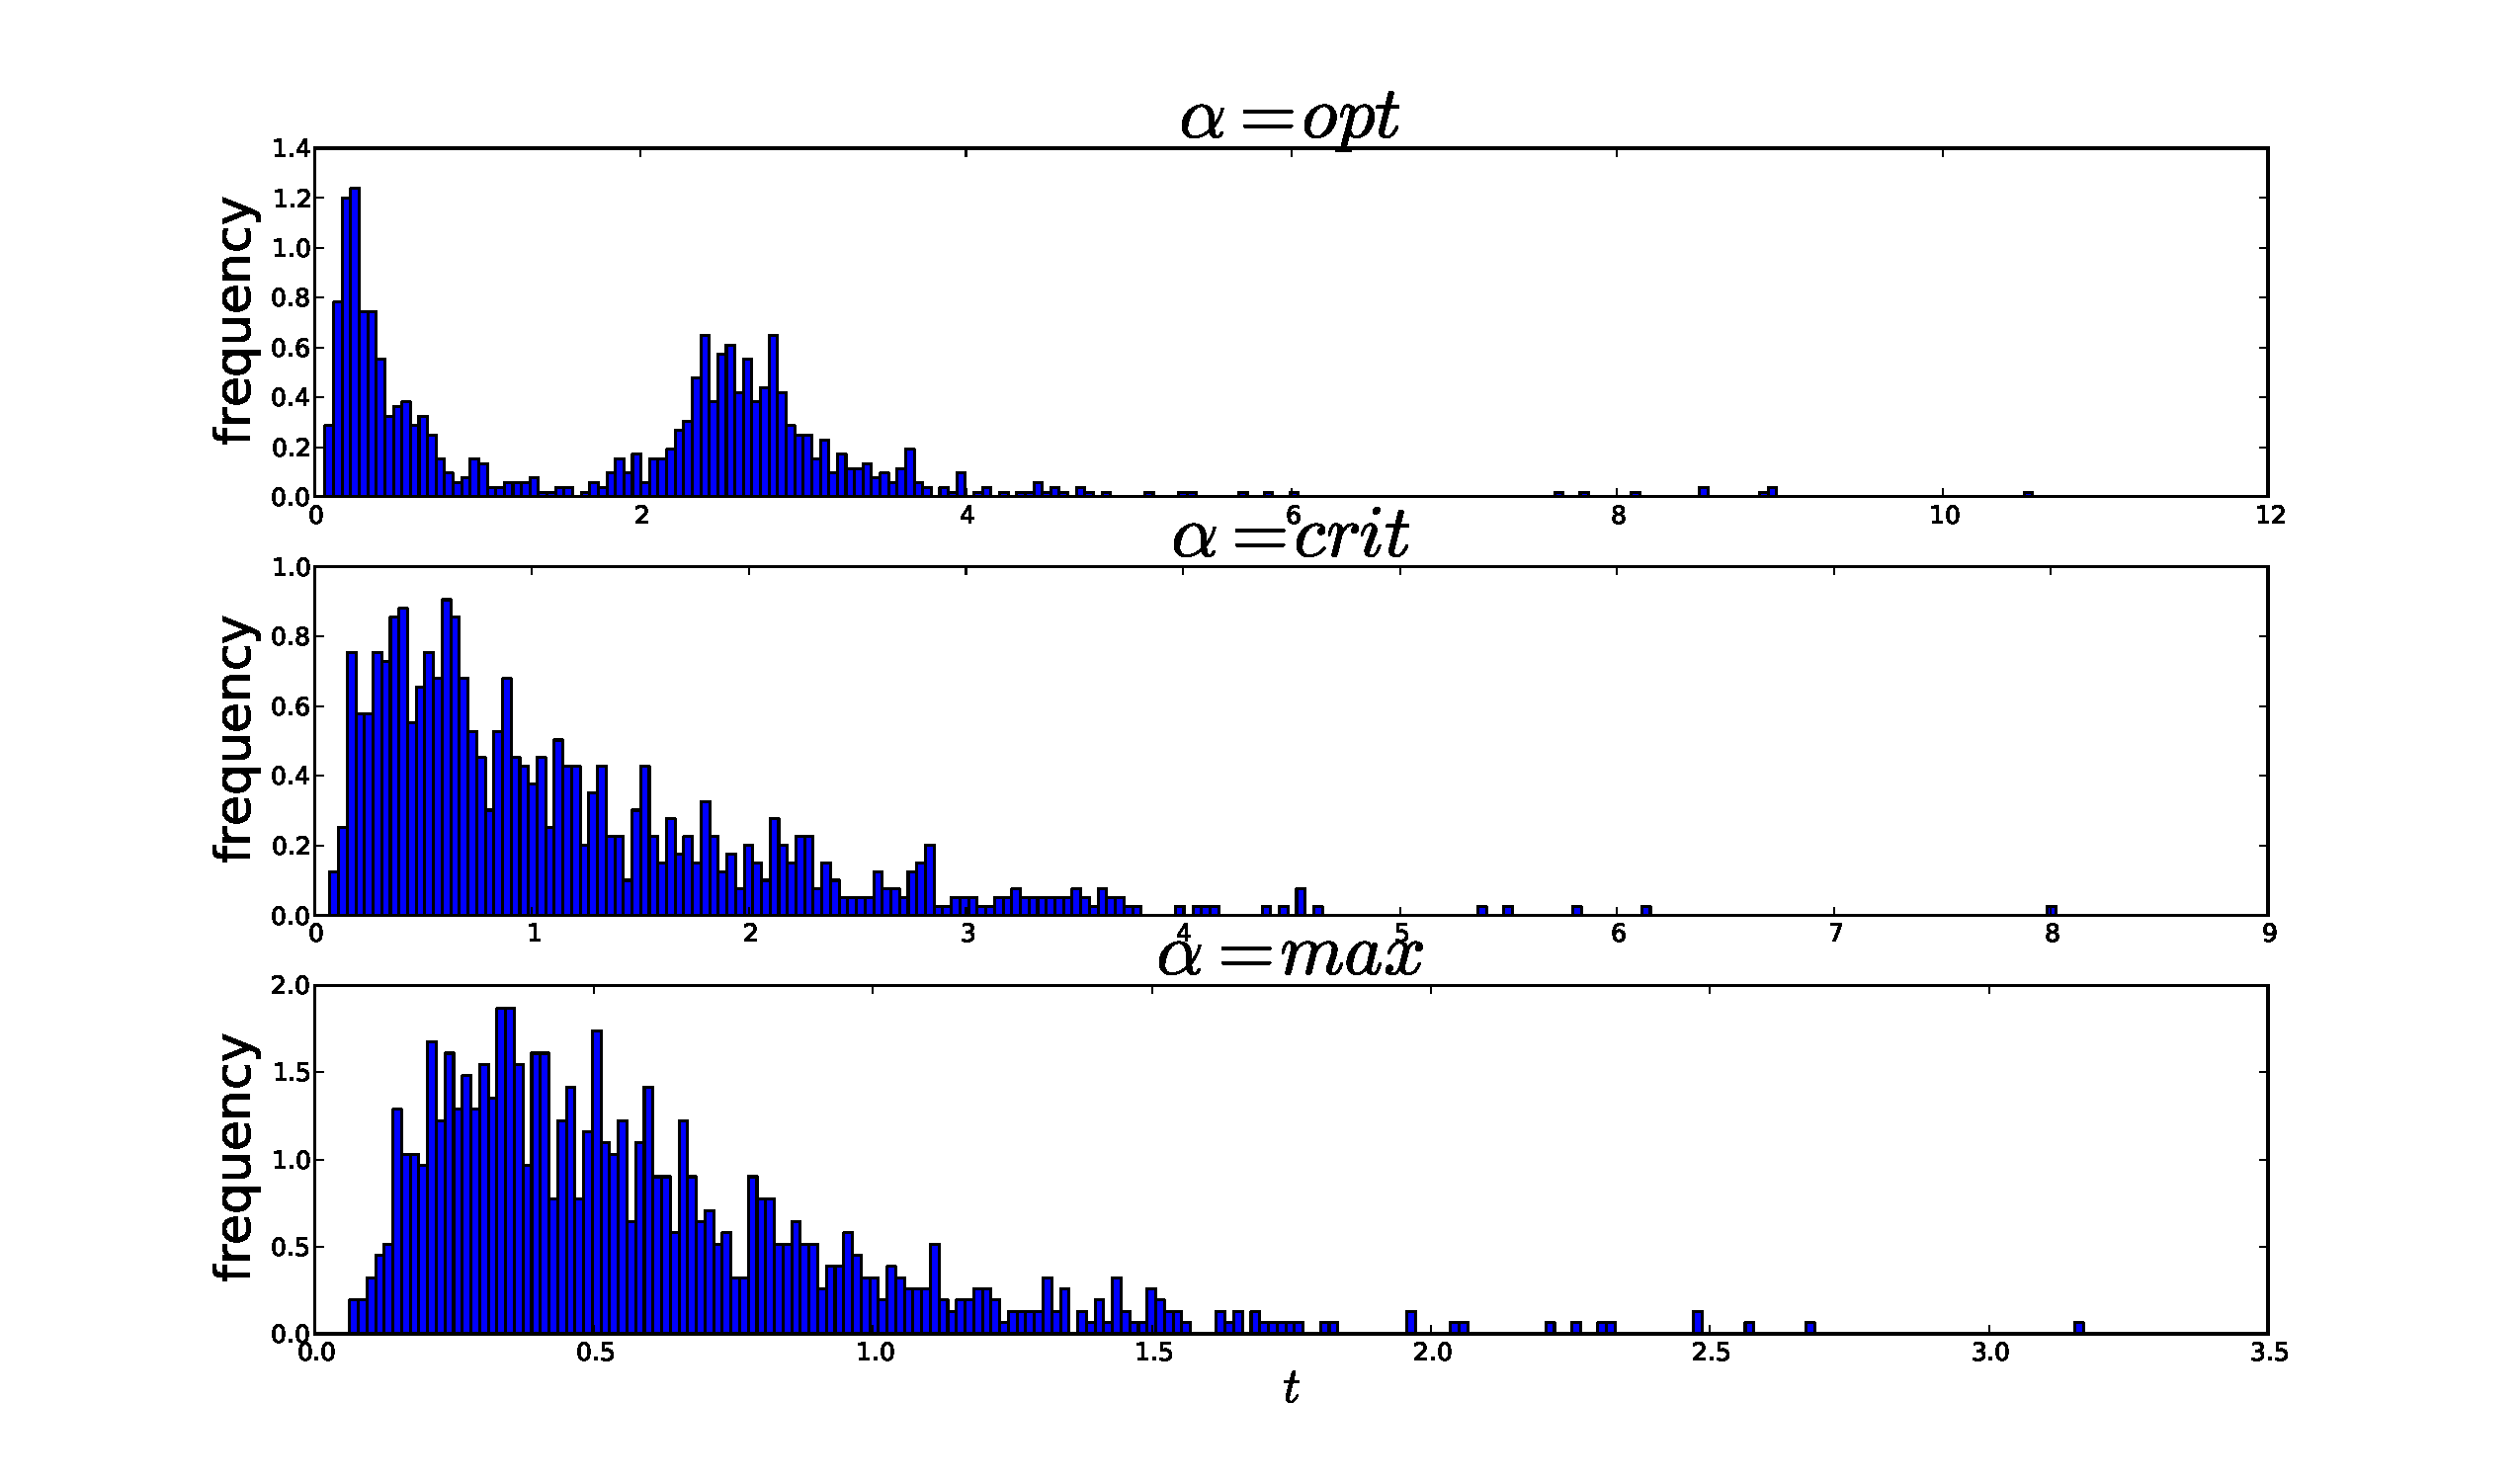
\includegraphics[width=\textwidth]{Figs/HitTime_MI_TauChar_Adjoint_Estimate/three_pt_prior_thits_distn.pdf}
%   \caption[labelInTOC]{Empirical Hitting-TIme distributions for the different
%   choices of $\a$}
%   \label{fig:empirical_hitting_times_3alphas}
% \end{center}
% \end{figure}

The estimation results are tabulated in in
\cref{tab:beta_estimates_from_hitting_times_different_alphas}.

\begin{table}
% \subfloat[$N_b=1000, N_s = 1e2$]{
% \begin{tabular}{ccc}
% \input{../OptEstiamte/Figs/HitTime_MI_TauChar_Adjoint_Estimate/tauchar_hit_time_100.txt}
% \end{tabular}
% }
% \subfloat[$N_b=100, N_s = 1e3$]{
% \begin{tabular}{ccc}
% \input{Figs/HitTime_MI_TauChar_Adjoint_Estimate/tauchar_hit_time_1000.txt}
% \end{tabular}
% }\\
% \subfloat[$N_b=10, N_s = 1e4$]{
% \begin{tabular}{ccc}
% \input{Figs/HitTime_MI_TauChar_Adjoint_Estimate/tauchar_hit_time_10000.txt}
% \end{tabular}
% } 
% \subfloat[$N_b=1, N_s = 1e5$]{
% \begin{tabular}{ccc}
% \input{Figs/HitTime_MI_TauChar_Adjoint_Estimate/tauchar_hit_time_100000.txt}
% \end{tabular}
% }
\caption[Batch $\tau$ MLE estimates]
{Results for the estimates arising from simulations using various values of $\a$
(opt, crit, max). In each sub-table there are $N_b$ parameter estimates for each distinct $\a$, with $N_s$ hitting times used to
form a $\tc-$estimate.  The 'true' value of $\tc$ is $\tc=1$. 
Also see \cref{fig:beta_estimates_from_hitting_times_different_alphas}.}
\label{tab:beta_estimates_from_hitting_times_different_alphas} 
\end{table}   

\begin{figure}[h]
\begin{center}
\subfloat[$N_b=1e3, N_s = 1e2$]
{
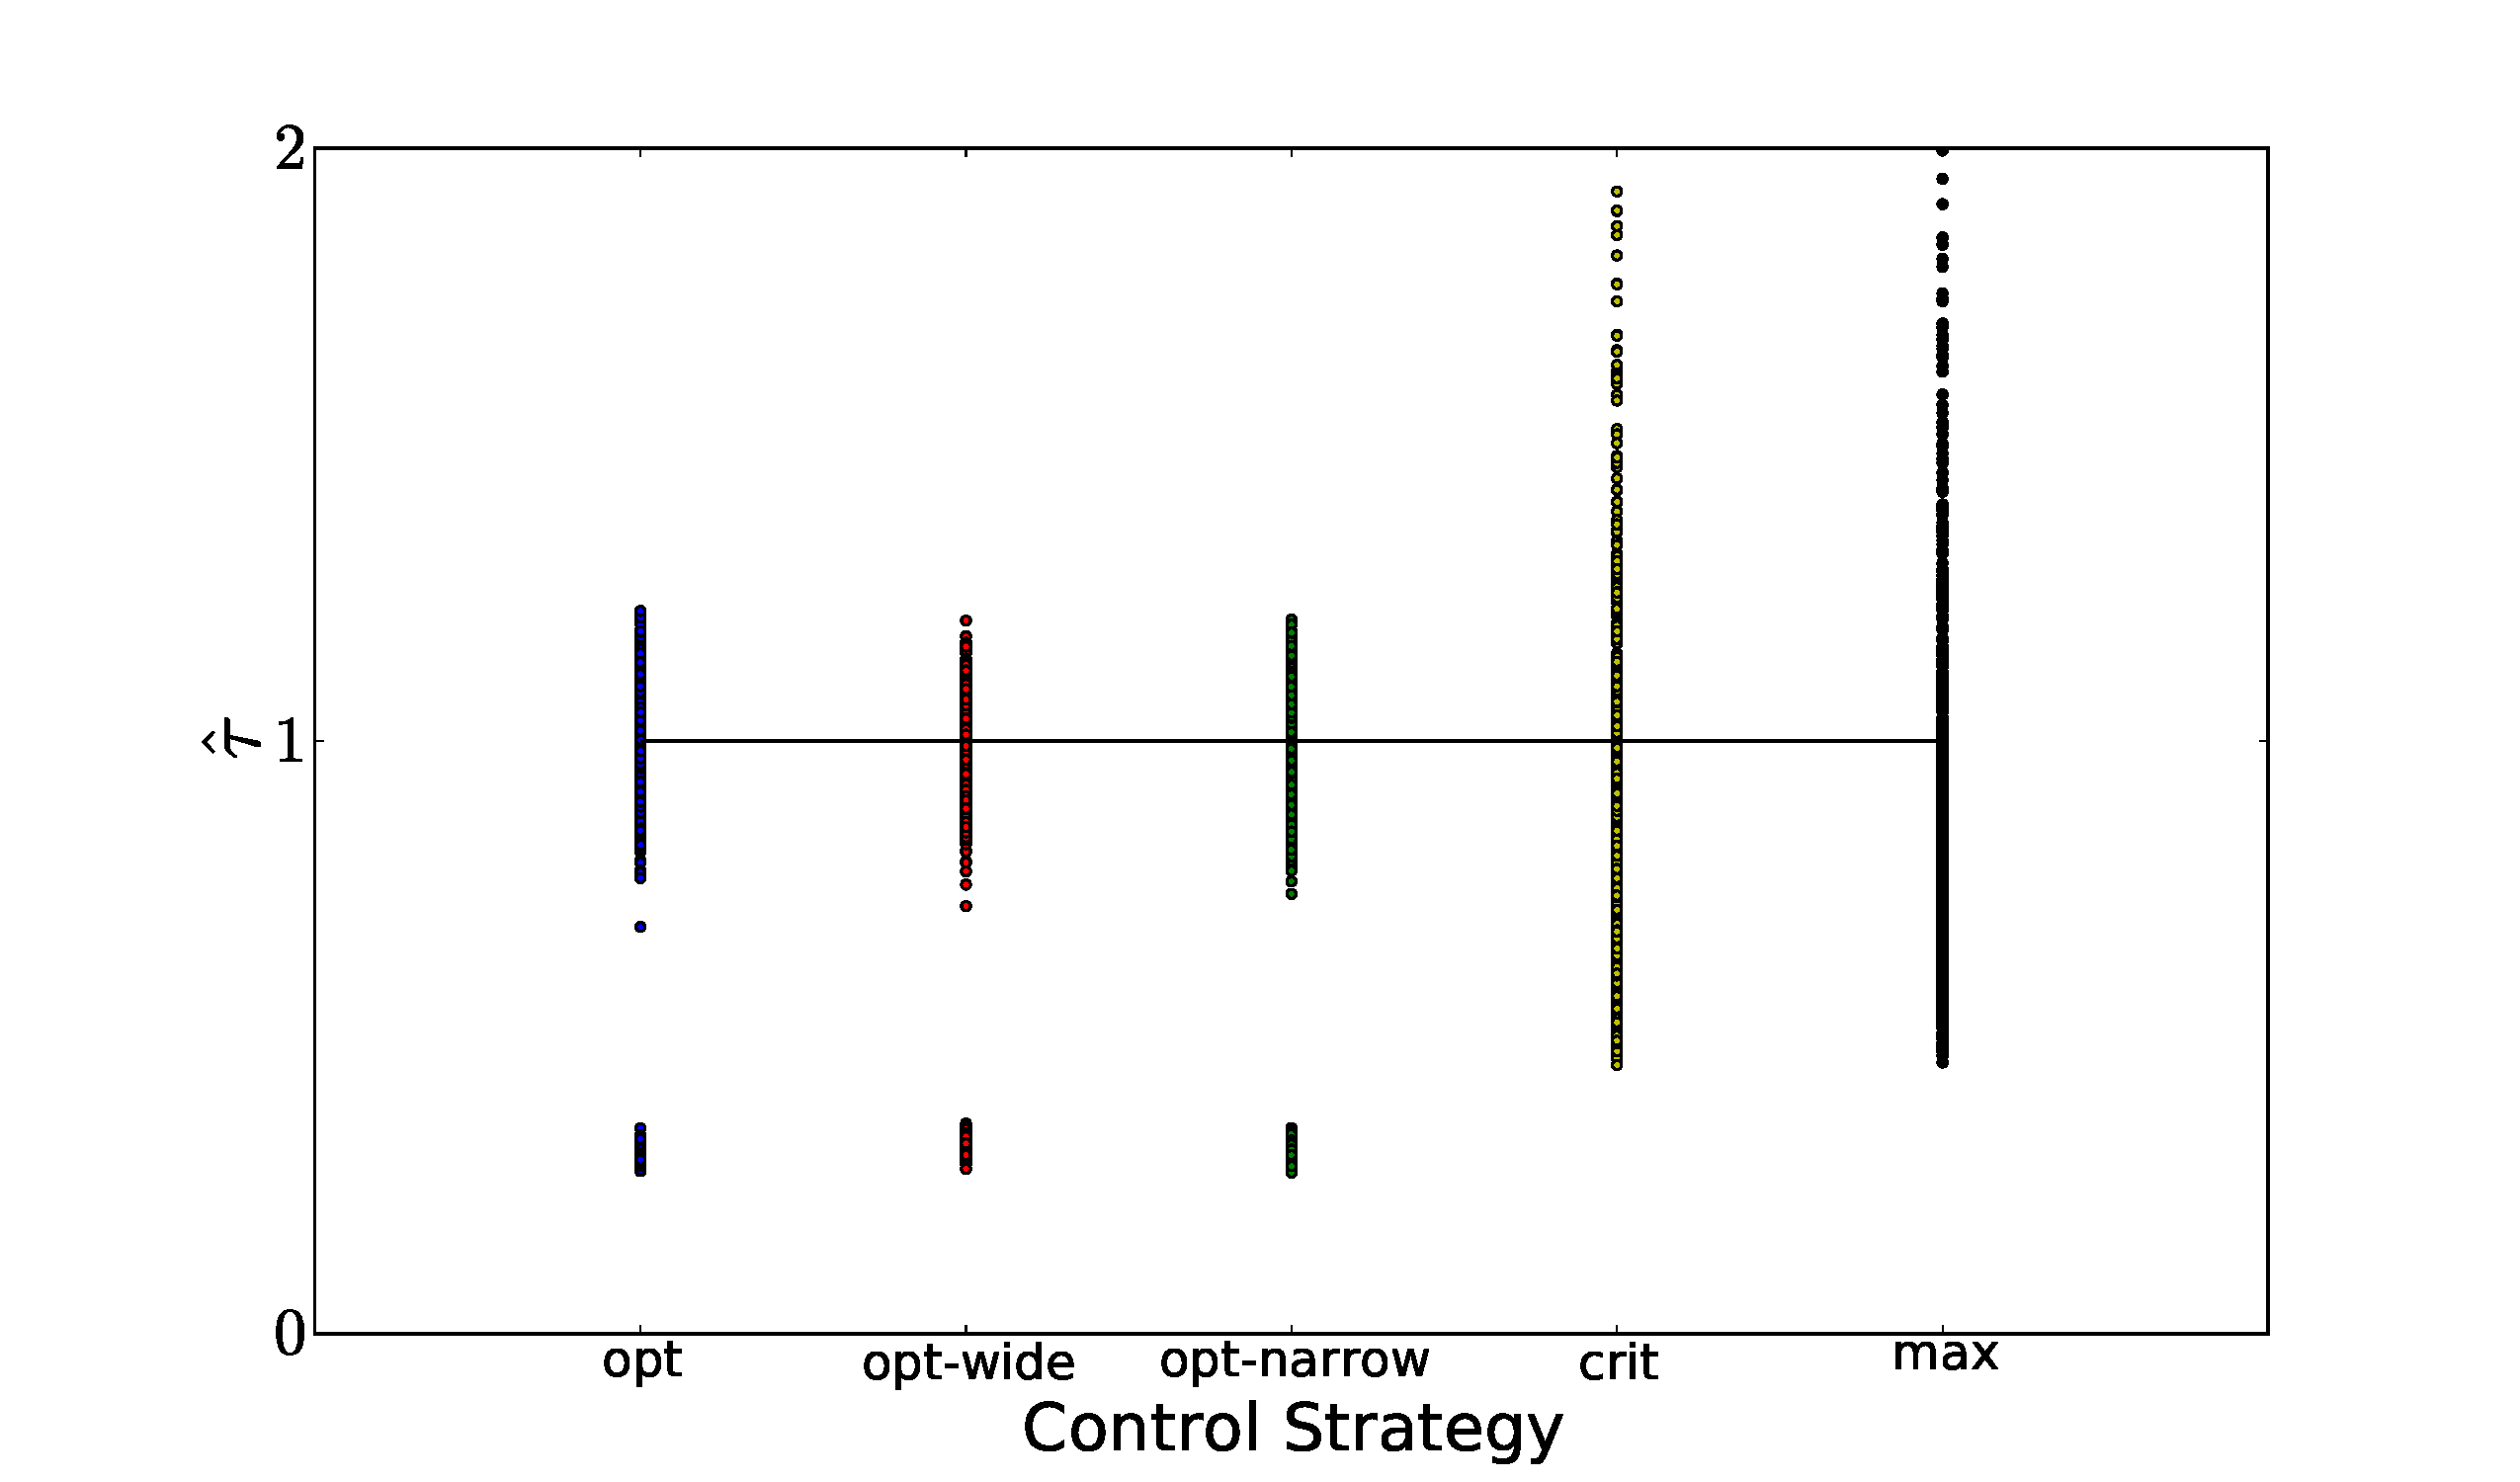
\includegraphics[width=0.48\textwidth]
{Figs/HitTime_MI_TauChar_Adjoint_Estimate/miestimates_scatterplot_Nb1000_Ns100.pdf}
}
\subfloat[$N_b=1e2, N_s = 1e3$]
{
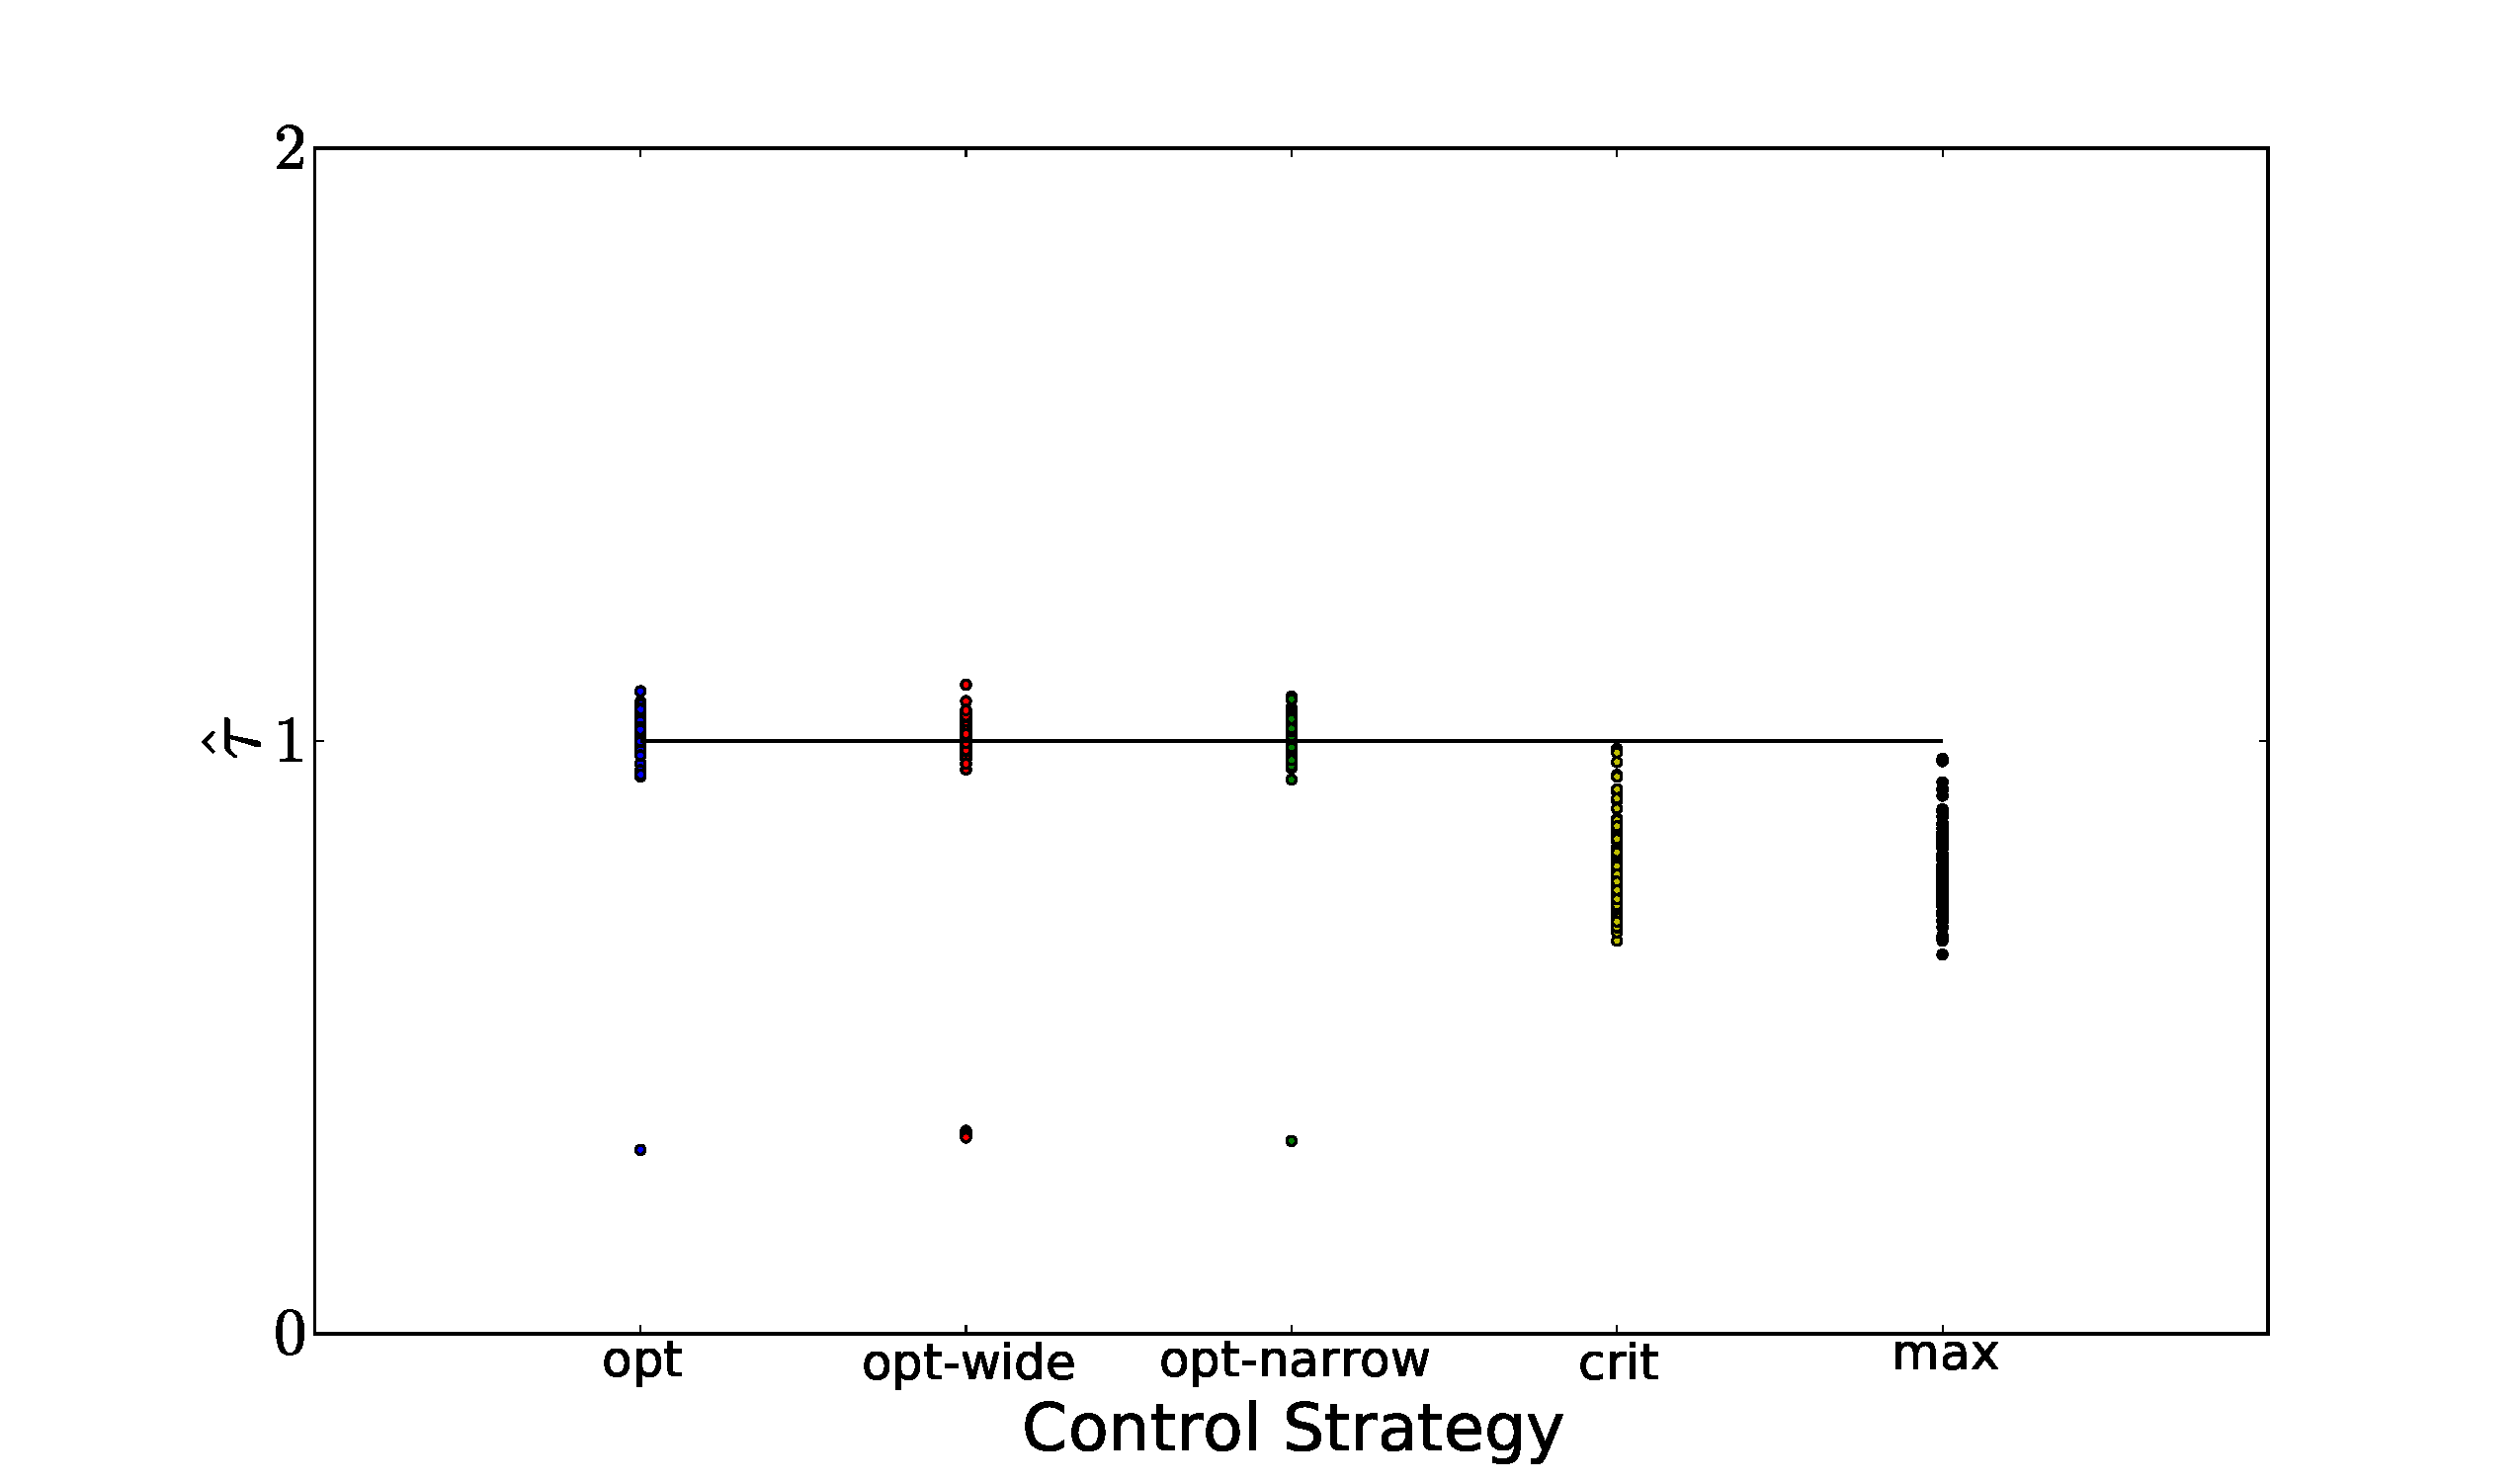
\includegraphics[width=0.48\textwidth]
{Figs/HitTime_MI_TauChar_Adjoint_Estimate/miestimates_scatterplot_Nb100_Ns1000.pdf}
}
\\
\subfloat[$N_b=1e2, N_s = 1e4$]  
{
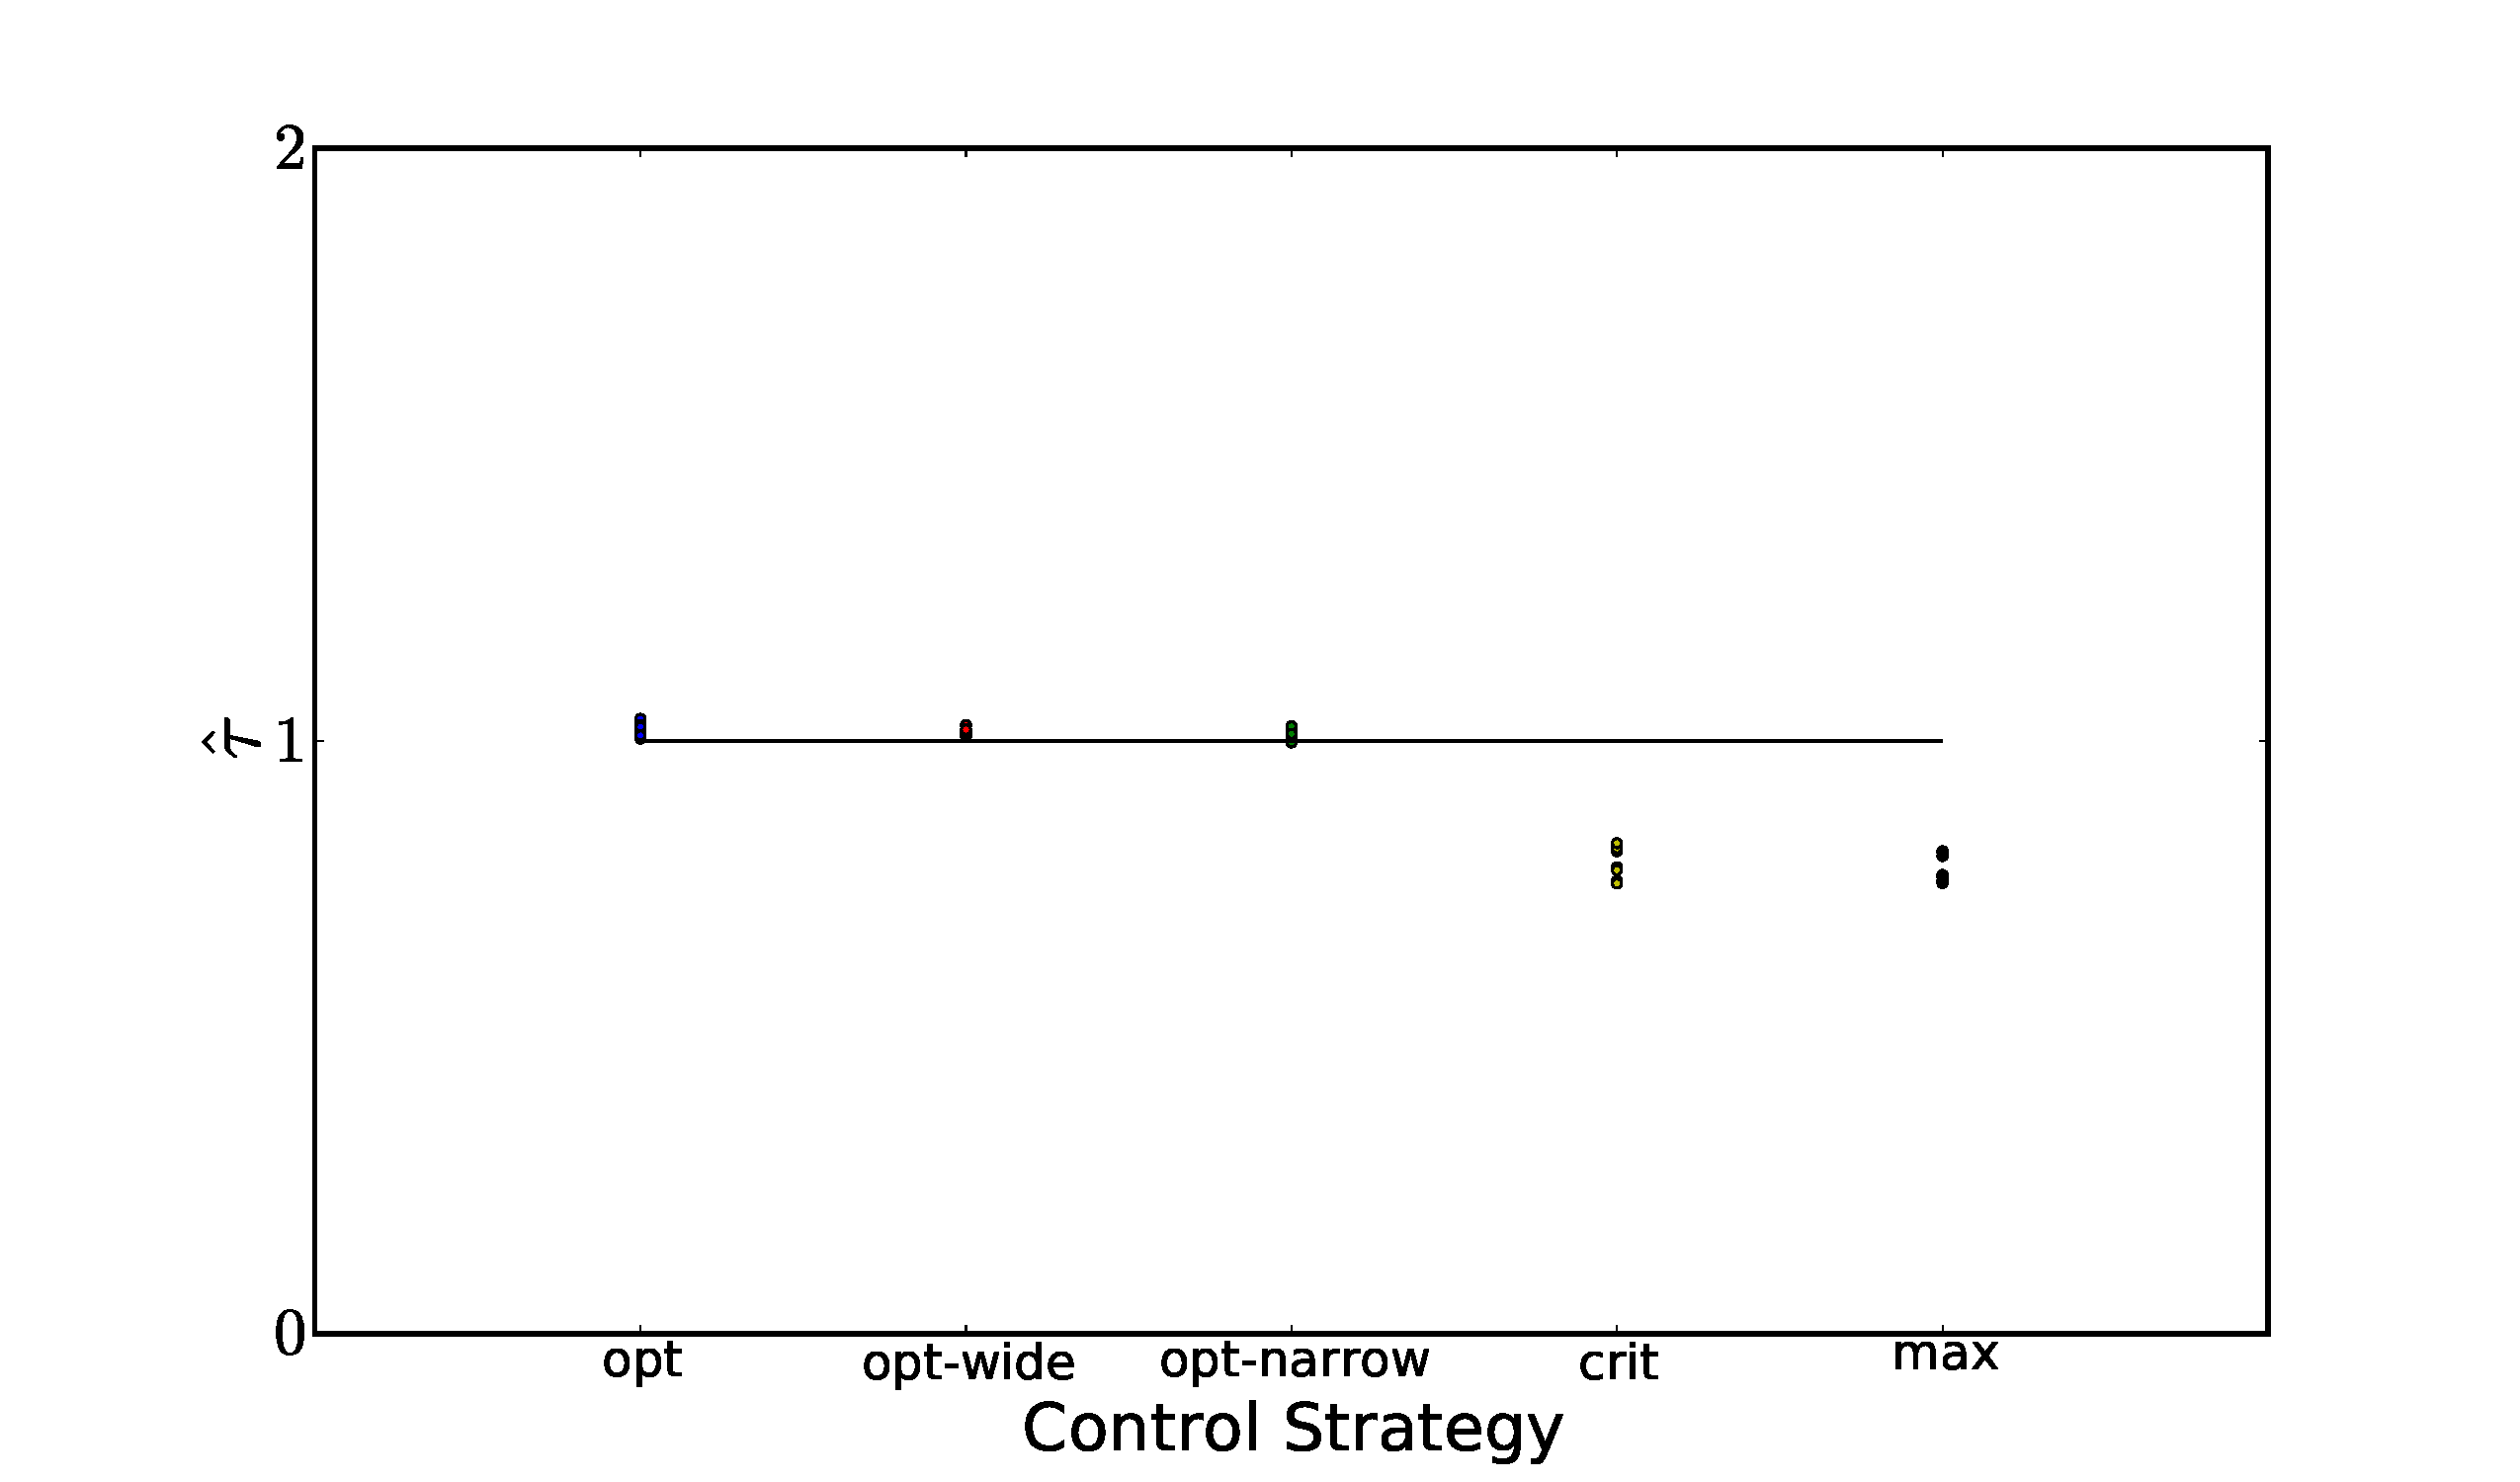
\includegraphics[width=0.48\textwidth]
{Figs/HitTime_MI_TauChar_Adjoint_Estimate/miestimates_scatterplot_Nb10_Ns10000.pdf}
}  
\subfloat[$N_b=1e1, N_s = 1e5$]
{ 
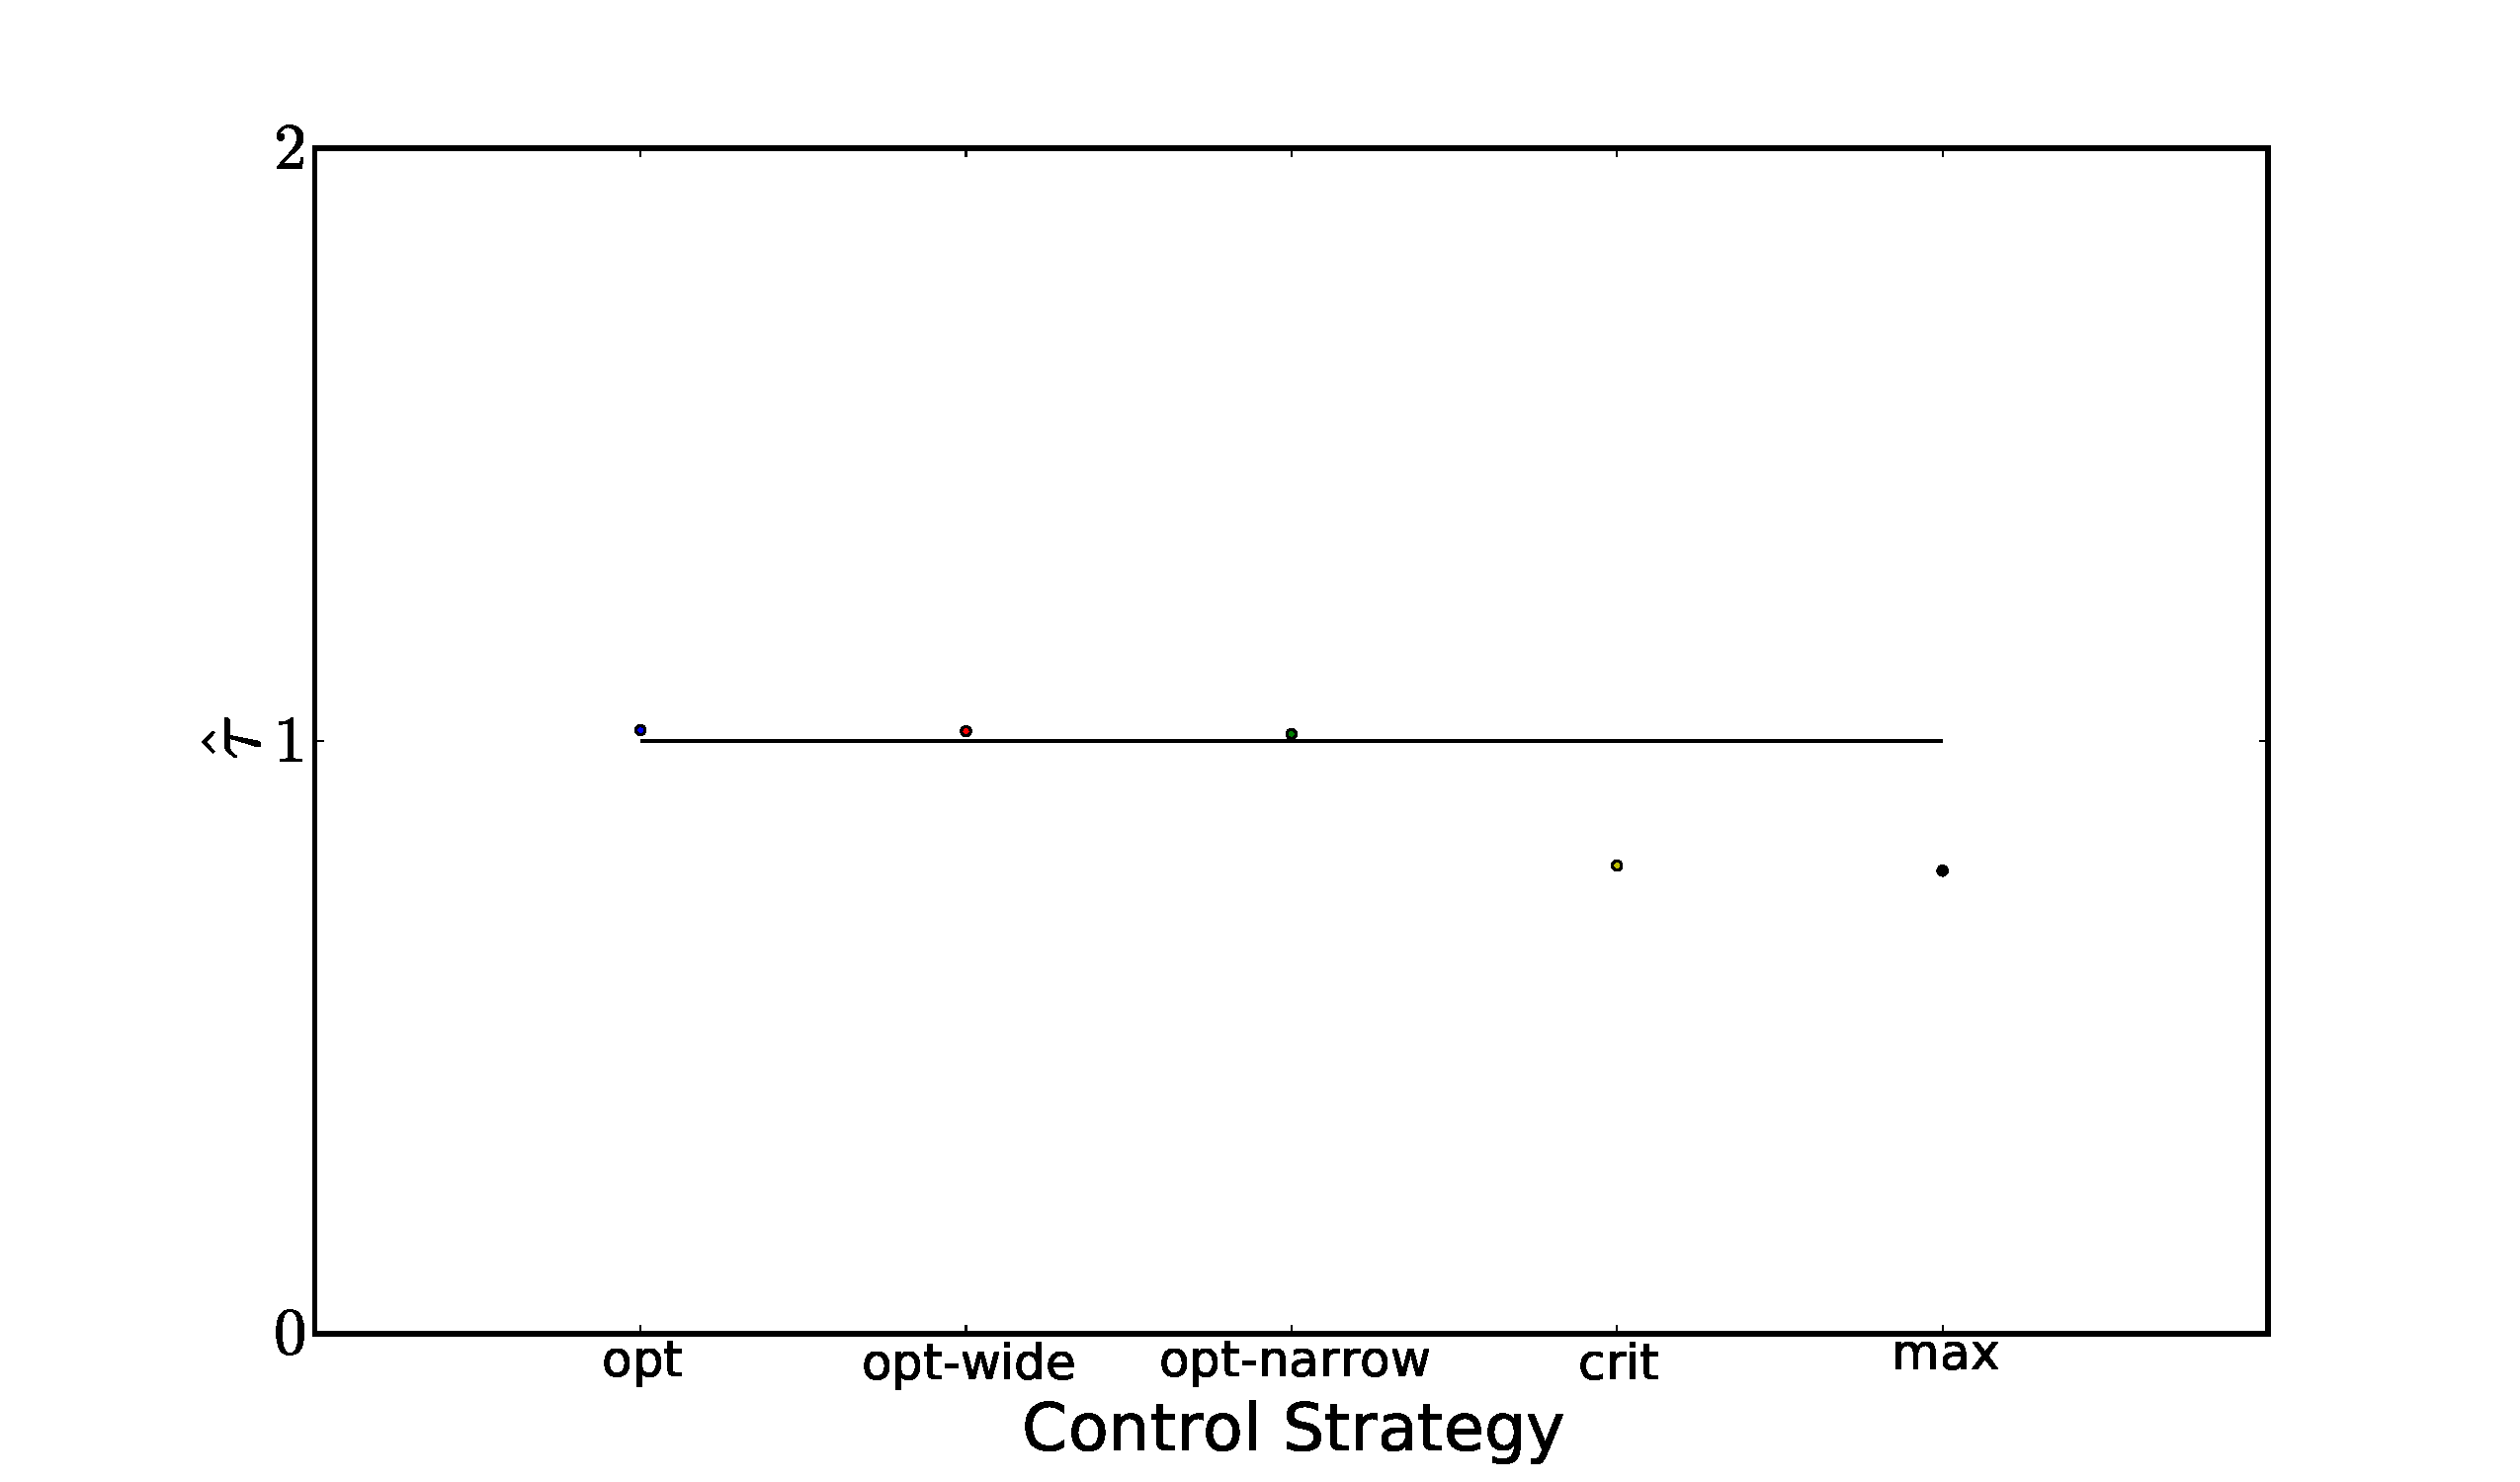
\includegraphics[width=0.48\textwidth]
{Figs/HitTime_MI_TauChar_Adjoint_Estimate/miestimates_scatterplot_Nb1_Ns100000.pdf}
}
\caption[Illustration of the individual MLE Estimates]{Fine Visualization of the
MLE estimates for the different controls, also see
\cref{tab:beta_estimates_from_hitting_times_different_alphas}}
\label{fig:beta_estimates_from_hitting_times_different_alphas}
\end{center}
\end{figure}
 
Given
\cref{tab:beta_estimates_from_hitting_times_different_alphas,fig:beta_estimates_from_hitting_times_different_alphas},
we see a clear advantage to using the Optimal Control, $\a_{opt}$ over the
simpler, constant controls. In particular, the bias of the estimates seems to
be significantly reduced. The variance is greater for the optimal controls, but
a look at the detailed distribution of estimates, top panels in
\cref{fig:beta_estimates_from_hitting_times_different_alphas} indicates that
this is due to a few outliers. Meanwhile, if we consider the various optimal
controls, 'opt' vs. 'opt-wide', 'opt-narrow', we see that there is no big
difference in the estimator quality of each - they all perform approximately
equivalently. 


\subsection{Closer look when the estimation goes wrong}
TODO: Move to appendix?

In general, the optimally-stimulated samples give (much) more accurate estimates
than the ones that are naively-stimulated. However, we see in
\cref{fig:beta_estimates_from_hitting_times_different_alphas}, panel b) that
occasionally (once), the optimally-stimulated sample can give very wrong
estimates.

We now plot what goes wrong in that sample vs. the base-case where the estimate
is almost exact, see \cref{fig:batch_estimtion_in_detail}. It seems that in the
bad case, there are enough extreme (very long) hitting times that the estimation
procedure infers that the characteristic time must be very small (i.e the
attractive force towards $\mu=0$ is very strong). In the larger sample, there
are no other examples of these extremely delayed hitting times, they are thus
seen to be a rarity and the correct parameter value is inferred.

\begin{figure}[h]
\begin{center} 
\subfloat[1e3 Hits]  
{ 
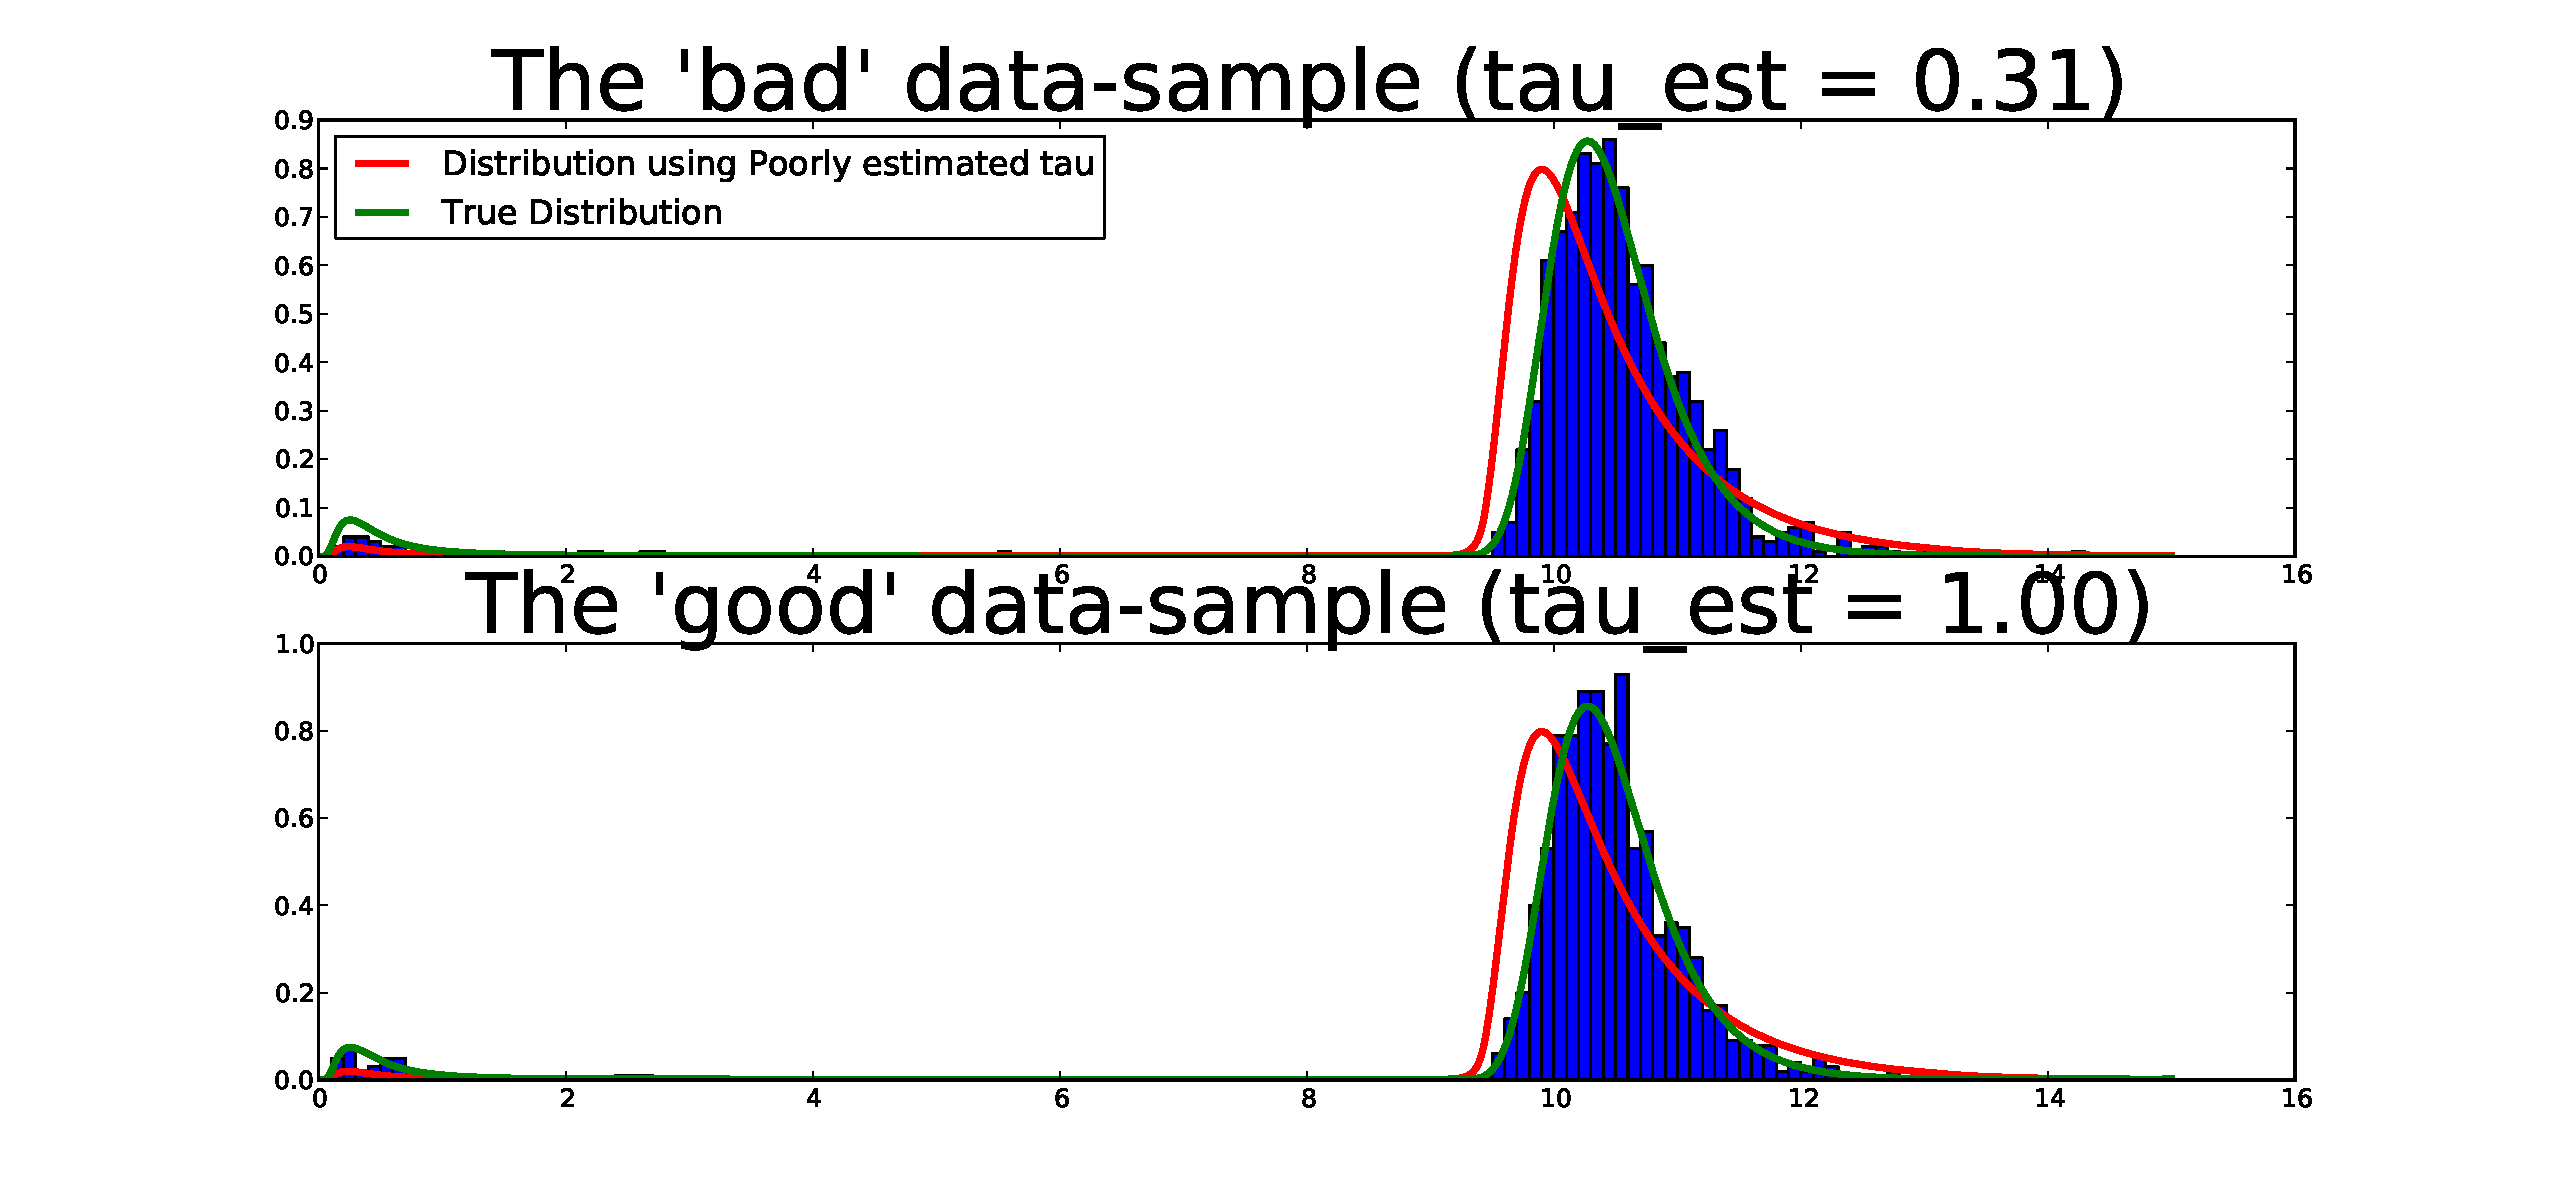
\includegraphics[width=0.98\textwidth]
{Figs/HitTime_MI_TauChar_Adjoint_Estimate/Adjoint_TauChar_Estimator_good_vs_bad_estimates_Nh1000.pdf}
}\\
\subfloat[1e4 Hits]
{
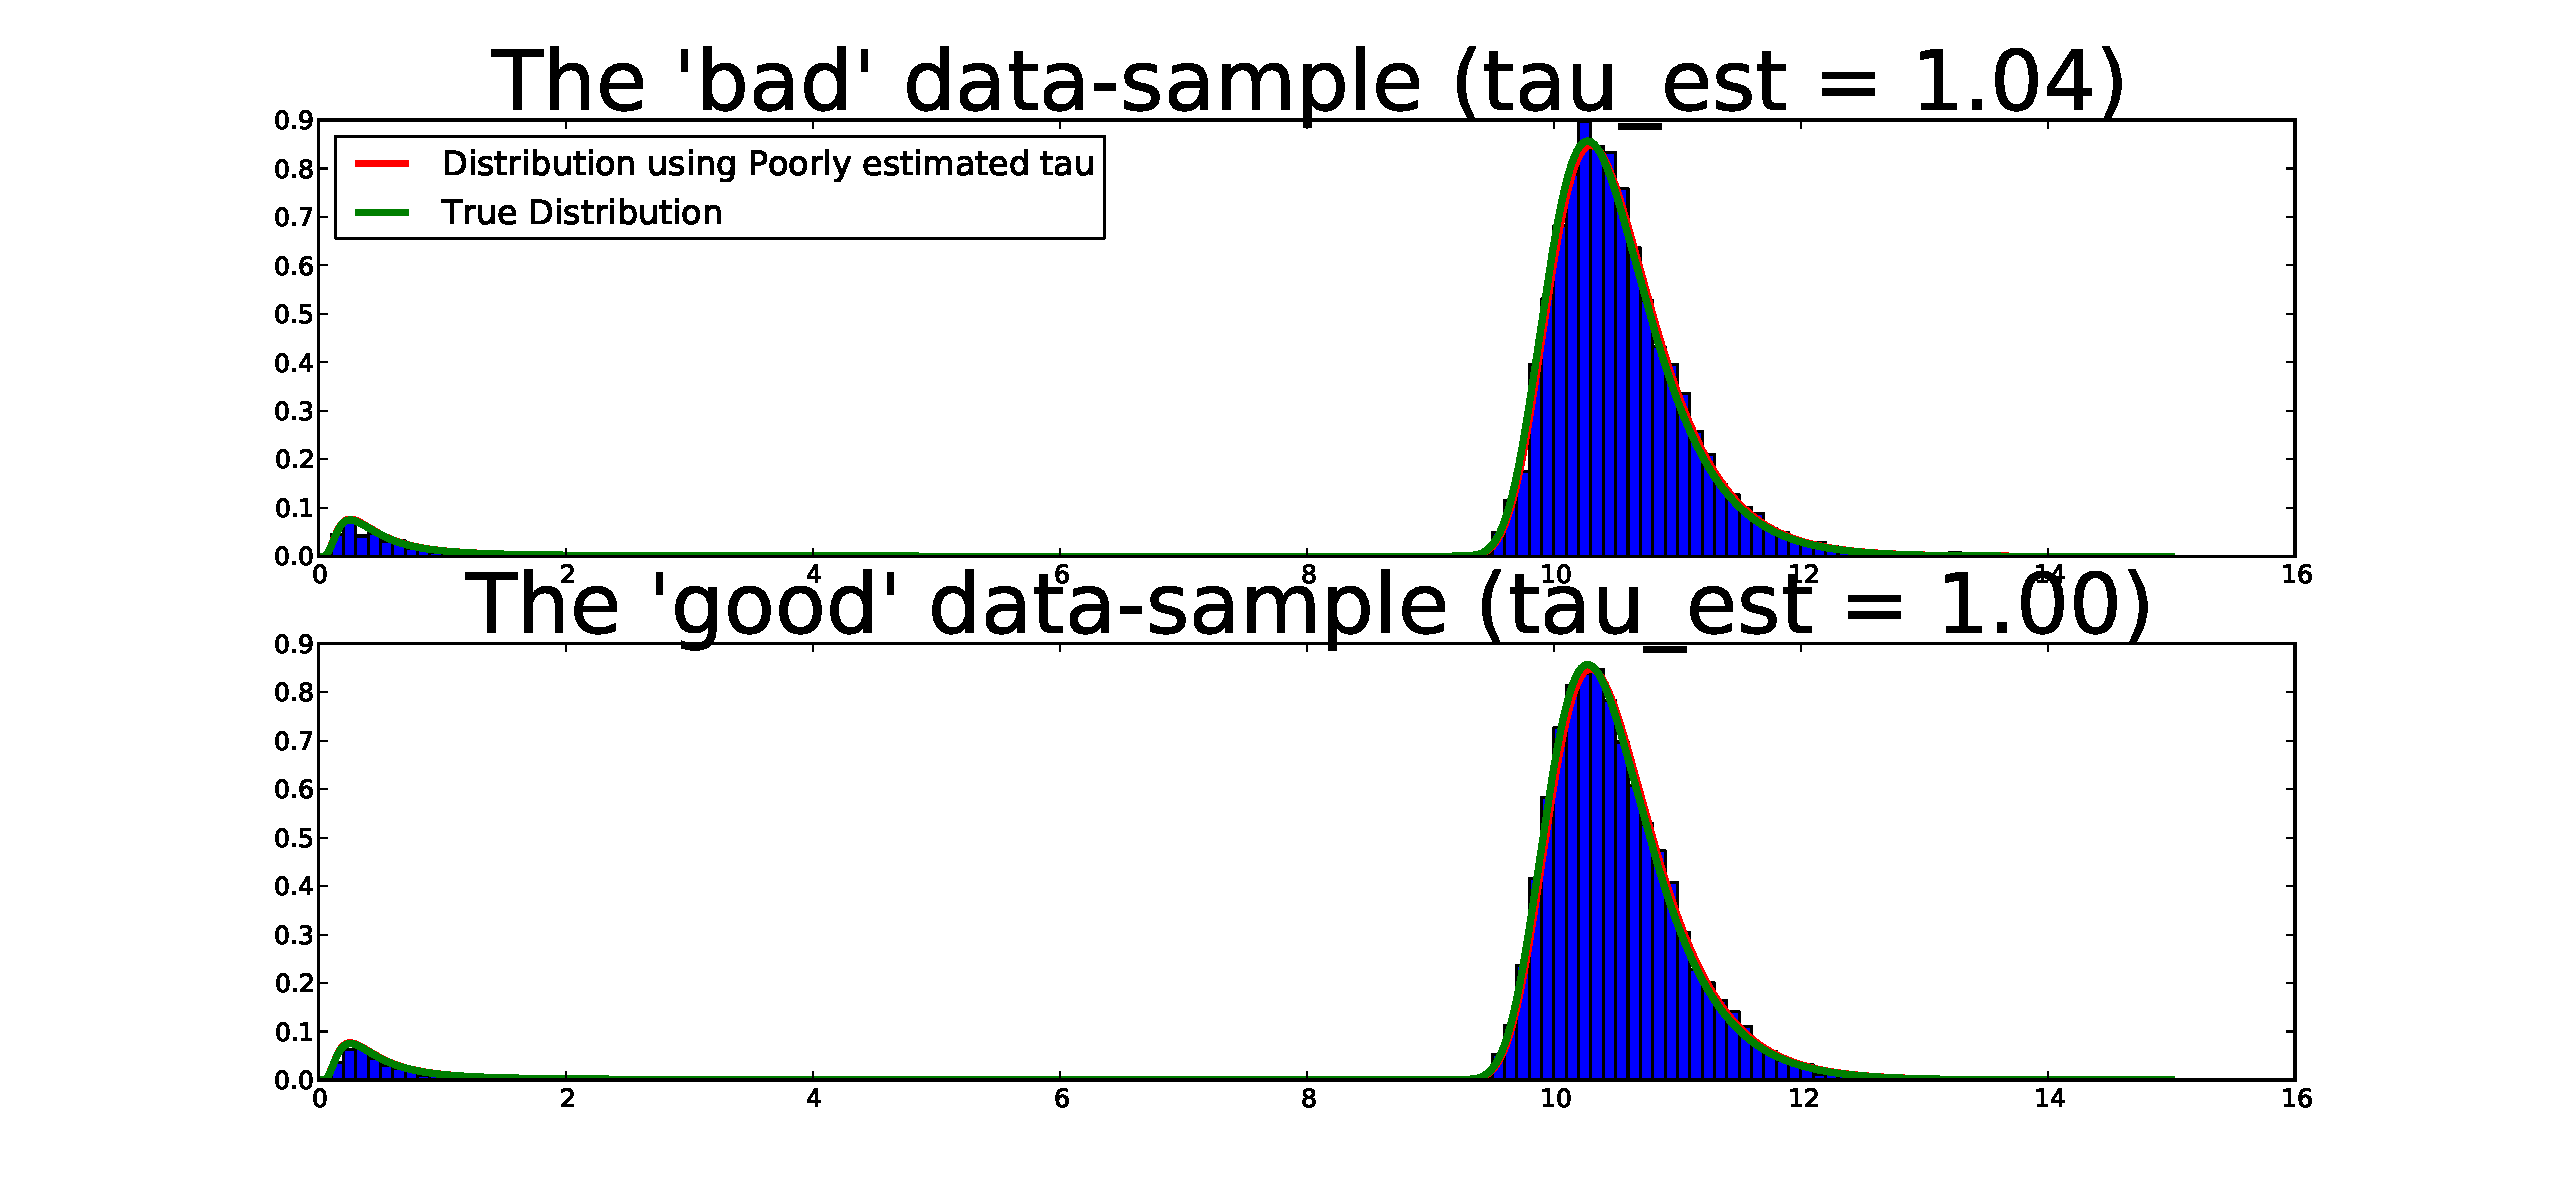
\includegraphics[width=0.98\textwidth]
{Figs/HitTime_MI_TauChar_Adjoint_Estimate/Adjoint_TauChar_Estimator_good_vs_bad_estimates_Nh10000.pdf}
}
\caption[Estimation Detail View for the Optimally-Stimulated
Experiment]{Comparing the case when the estimation does best vs. when it does
worst for the optimally-stimulated experiment. In the case with less samples, a
few extreme observations can skew the estimate, however with more data points,
those are seen to be rare cases and a more accurate estimate is found.}
\label{fig:batch_estimtion_in_detail}
\end{center}
\end{figure}


\subsection{Proof of concept of estimating the entire parameter set}
So far we have assumed that $\mu, \s \in \th$ are known. We now relax that
assumption and attempt to estimate those two parameters in addition to
characterisitc time $\tc$. We still use the optimal control obtained assuming
$\m,\s$ known. Why is this expected to work? First of all we found that the
optimal control seems essentially irrelevant to the exact values of $\m,\s$ as
long as they are not 'too far' from the nominal values ($\m=0, \s=1$.). Moreover
as discussed in the introduction, the $\tc$ parameter is well-known to be the
hardest to estimate. Thus a scheme designed to estimate it well is conjectured
to help with estimation of the entire parameter set, since removing variation
from one parameter estimate necessarily removes variation from the others.

We use the same simulated hitting-time data-set as in
\cref{tab:beta_estimates_from_hitting_times_different_alphas,fig:beta_estimates_from_hitting_times_different_alphas},
using $N_s=1e4$ hits and $N_b=10$ separate sample-sets, i.e.\ we make 10
estimates.

The results are given in \cref{fig:all_theta_estimates_batch}, it is clear that
the 'optimally' stimulated samples result in much more accurate and precise
estimates. In particular all stimulation schemes come-up with high-fidelity
estimates for $\s$, it is in resolving the interplay between $\m,\tc$ that the
'optimal' stimulation excels. In particular the 'naive' stimulations does
not allow to distinguish a high $\m$ and a small $\tc$ from a low $\m$
and a high $\tc$, while the dynamic, bang-bang situation makes it possible.

\begin{figure}[htp]
\begin{center}
  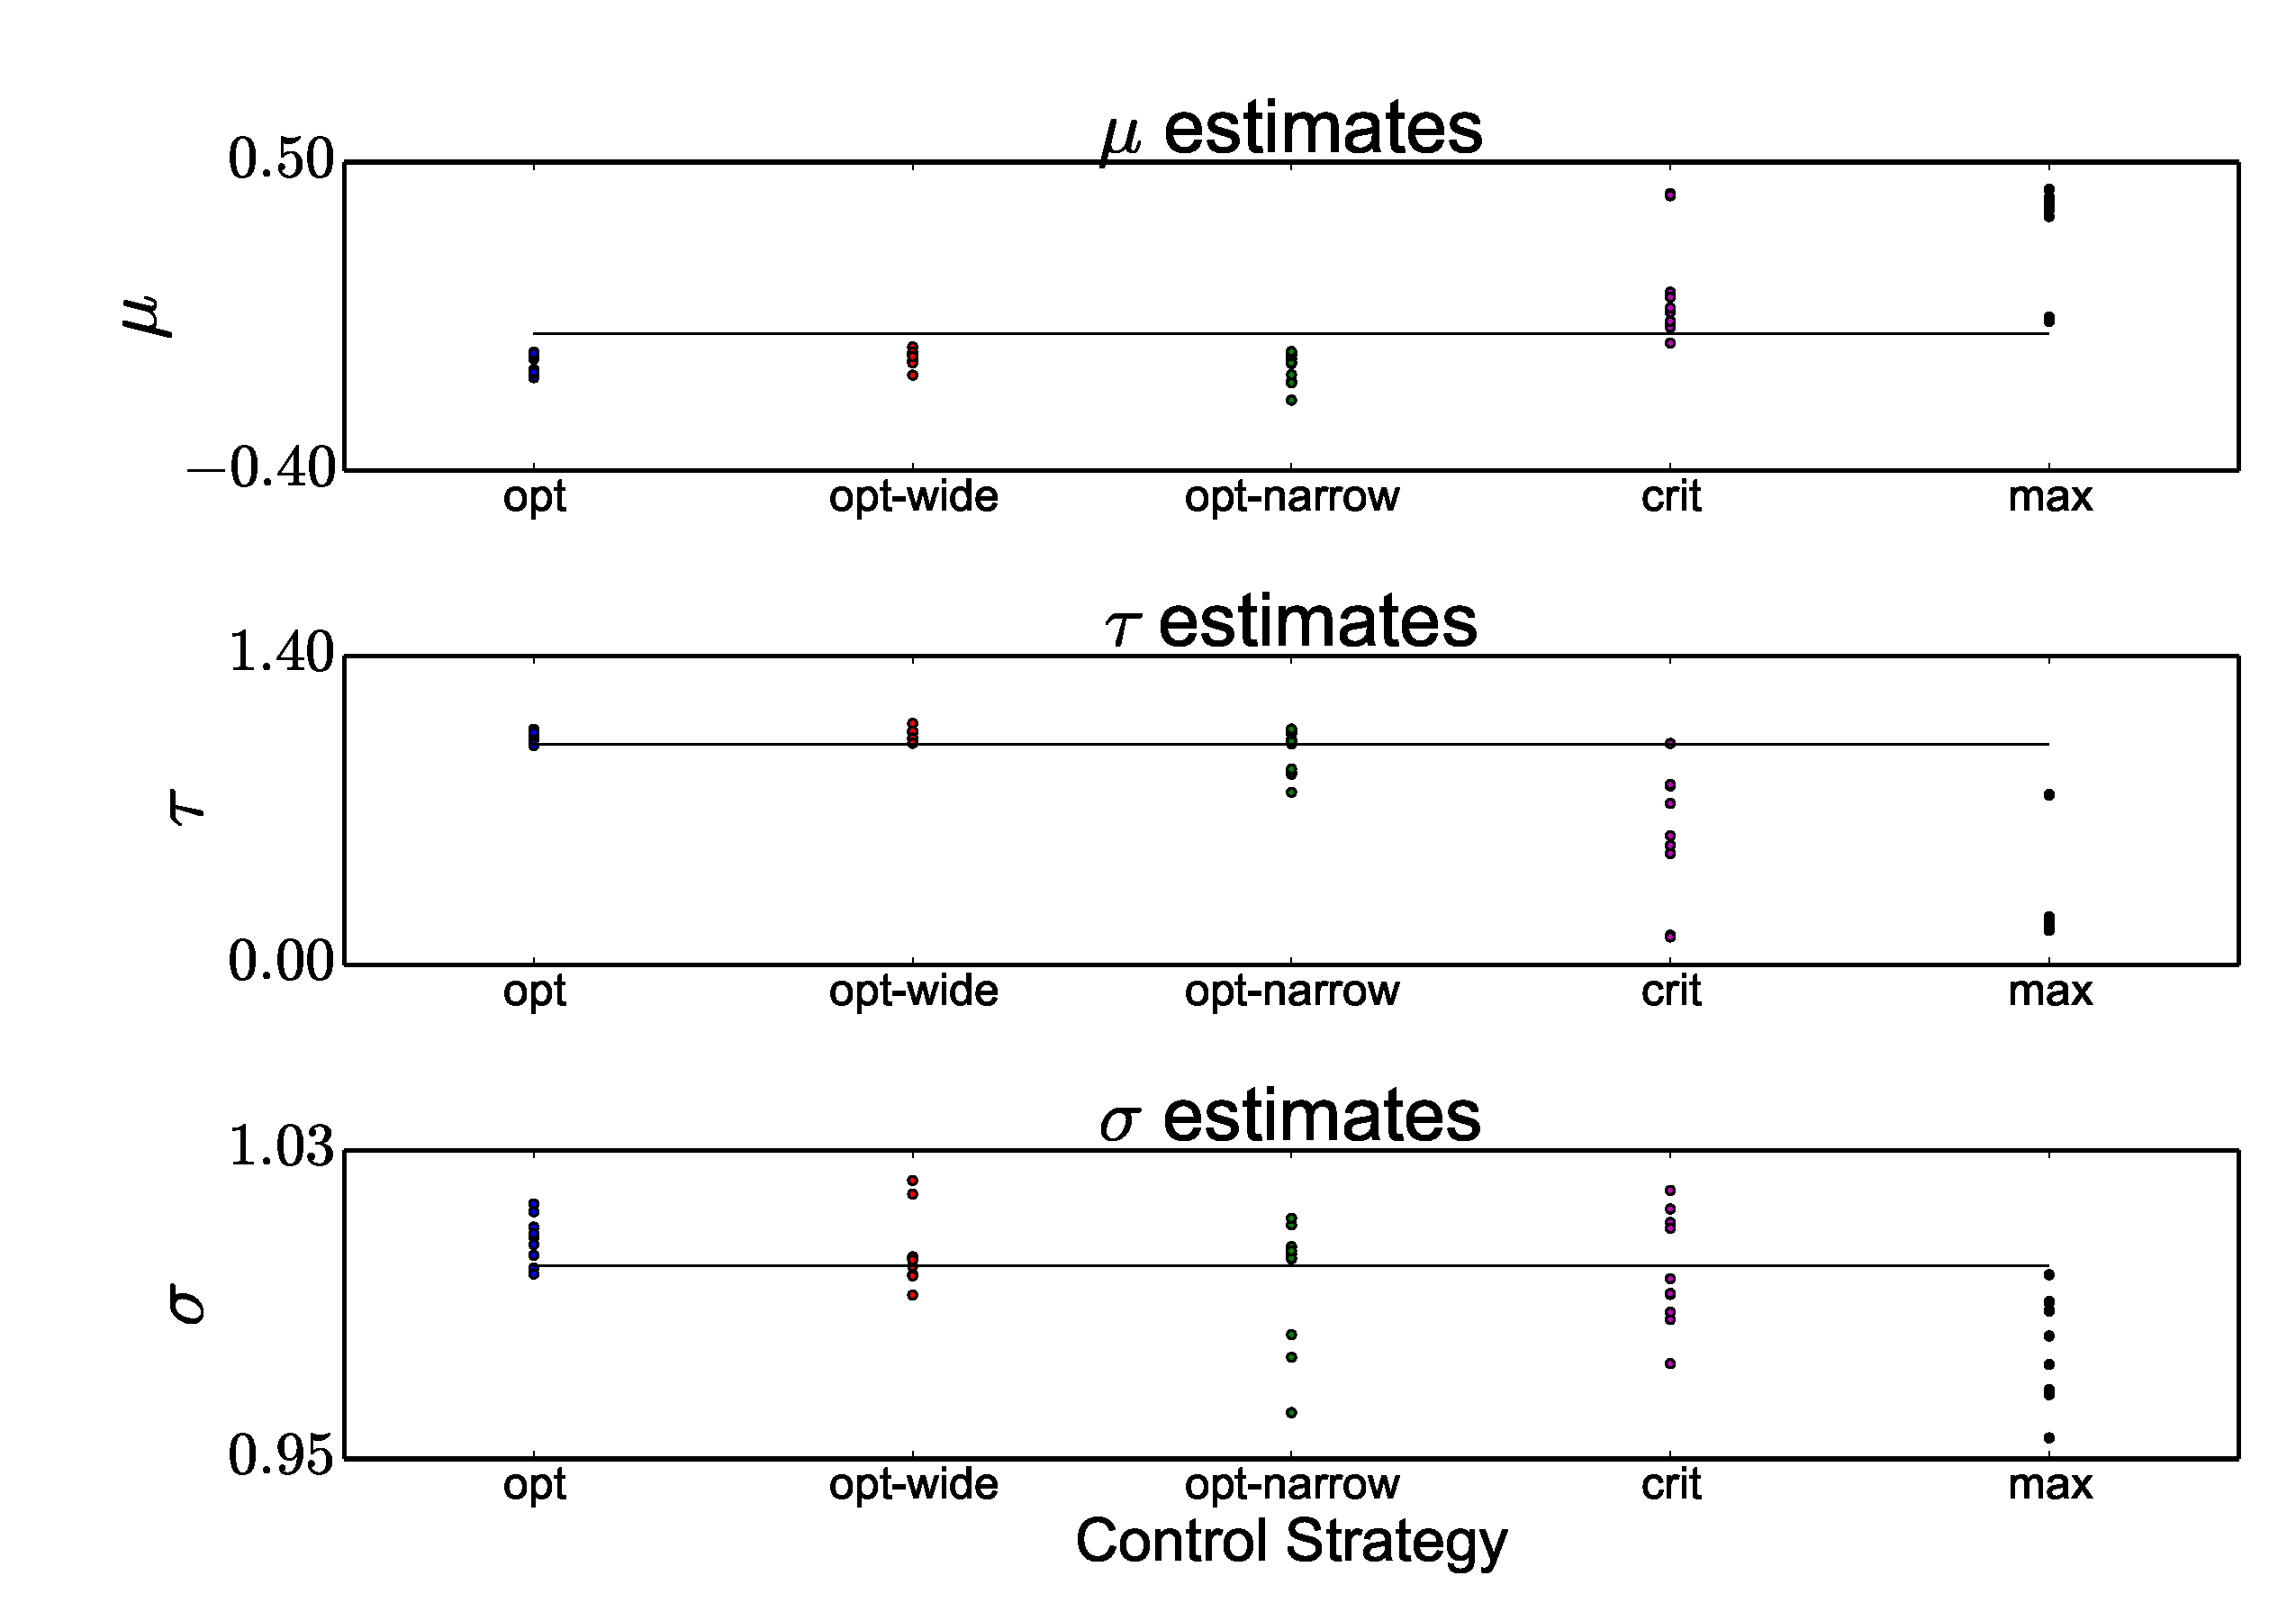
\includegraphics[width=\textwidth]{/home/alex/Workspaces/Latex/OptEstimate/Figs/MuTauSigma_Batch_estimates/all_theta_estimates_scatterplot_Nb10_Ns10000.pdf}
  \caption[Batch estimates for all 3 parameters]{Optimal Stimulation greatly
  improves estimates when all parameters are being estimated. 
  From the top to bottom, we show $N_b=10$ estimates for $\m,\tc,\s$,
  formed after observing $N_s=1e4$ hits per-estimate. There are three 'optimal'
  stimulations as discussed in the text, shown to the left and two naive ones,
  shown to the right. The scatter dots are the individual estimates per
  stimulation-parameter pair. The horizontal line indicates the true value of
  the paramters, i.e.\ the value used to simulate the hitting-time observations
  in the data samples.}
  \label{fig:all_theta_estimates_batch}
\end{center}
\end{figure}

\clearpage

\section{Online Estimation}
\label{sec:online_estimation} 
In the {\sl online} optimization of the MI / estimation, we proceed in a
slightly more complicated way. In particular we 

\begin{enumerate}
  \item Find $\aopt$ using the gradient ascent, for the prior $\rho$
  \item Apply $\aopt$ and measure several $1,2\ldots,N_{s}$ hitting times
  $t_k$
  \item Update the $\rho$ into a posterior conditional on the observed $\{t_k\}$
  \item Recalibrate $\aopt$ using the new $\rho$, i.e. go back to 1. 
\end{enumerate}

In practice we incrementally, increase by starting with $N_s=1$ and then
doubling it, i.e.\ we re-compute $\a$ after the 1st, 3rd, 7th etc hitting time.

Computational efficiency considerations aside, we have already discussed and
illustrated all the techniques needed to perform pts. 1,2,4, it is
only the prior update that needs to be discussed.

\subsection{Quick Intro to Particle Filtering}
Recall Bayes' formula
$$
\rho(\th| \{t_k\} ) = 
\frac{  \rho(\th) \cdot \prod_k g(t_k|\th ; \a) }
	 { \int_\Th  \rho(\th) \cdot \prod_k g(t_k|\th ; \a)  \intd{\th}}
$$

In practice, exact calculation of $\rho(\th|\t_k)$ would not be possible in our
context, so an approximation approach needs to be made.

The standard approach is to describe the prior distribution by an ensemble of
points (particles). We now describe the basic aspect of how the particle
ensemble is constructed, how it is updated and how it is resampled. We use the
reference \cite{Granade2012}, in particular section 4 therein.

We have a prior
$ \rho(\th)$, which we represent or approximate  via an ensemble of points $\th_i$. as 
$$ \rho(\th) \sim \sum_i w_i \delta(\th-\th_i)$$
This is what we have been doing up to now for the MI optimization routines.

Again recall that a bayesian update, given the $k$th hitting time is
$$ \rho(\th|t_k) \propto g(t_k|\th)\rho(\th)$$

thus the weights are iteratively updated as 

$$w_i \ra w_i g(t_k|\th_i)$$

Given the particle ensemble, $\{\th_i, w_i\}$, we can  then approximate the
mean/variance of $\Th$ as
$$ \Exp[\Th] \approx \sum_i w_i \th_i$$
and 
$$ \Var[\Th] \approx \sum_i w_i \th_i \th_i - (\Exp[\Th])^2$$
In fact, in general 
$$\Exp[f(\Th)]\approx\sum_i w_i f(\th_i)$$ approximates the expectation of any
function, $f$, of the random variable $\Th$.

Here's the crux of the update/resample algorithm. Given a new observation, i.e.
the latest hitting time $t_k$, the weights are updated according to
$$ w_{i,k} = w_{i,k-1}\cdot g(t_k| \th_i, \a_k),$$where $g(|\th_i, \a_k)$ is
the probability density given the parameter value $\th_i$ and the chosen
stimulation that was applied during the $k$th sample, $\a_k(\cdot)$.
The weights are then re-normalized so that at all time $$\sum_i w_i = 1$$ 

The literature suggests that this procedure will tend to concentrate all the
'mass' on one location and most of the weights will decrease to 0. This
concentration is 'bad' since eventually, all the weights go to zero and so
effectively the distribution has converged  artificially to a point, which might
be the most likely point from the initial ensemble, but still be far from the
'true' value of the parameter. This adverse effect can be ameliorated by
resampling the {\sl locations} of the particle ensemble, $\th_i$. This
resampling can be done in many ways, but a standard way is described in
algorithm. \ref{alg:particle_resampling} (which is copied from Algo4 in Granade
et. al. \cite{Granade2012}, who in turn closely follow \cite{Liu2001}, but
are very nice and pedagogical).
While, of course, updating happens after every iteration, re-sampling happens
only when  
$$ \frac{1}{\sum_i^{N_p} w_i^2} < \frac {N_p}{2} \implies \textrm{ resample!}$$
For reference, the complete filtering algorithm is provided in 
Algorithm \ref{alg:particle_resampling} in the Appendix.



% In \cref{fig:poissonian_rate_filtering} we give an example for the filtering
% procedure to estimate the rate of a Poissonian process, $1/\t$, for which  the
% likelihood is just $\tfrac 1\t exp(- \tfrac t\t)$. From
% \cref{fig:poissonian_rate_filtering} we can conclude that the basic mechanics of
% the filtering update/resample procedure is working. (We've tried it with other
% values of $\tau$ and it works for those as well.)
% 
% %\usepackage{graphics} is needed for \includegraphics
% \begin{figure}[htp]
% \begin{center}
%   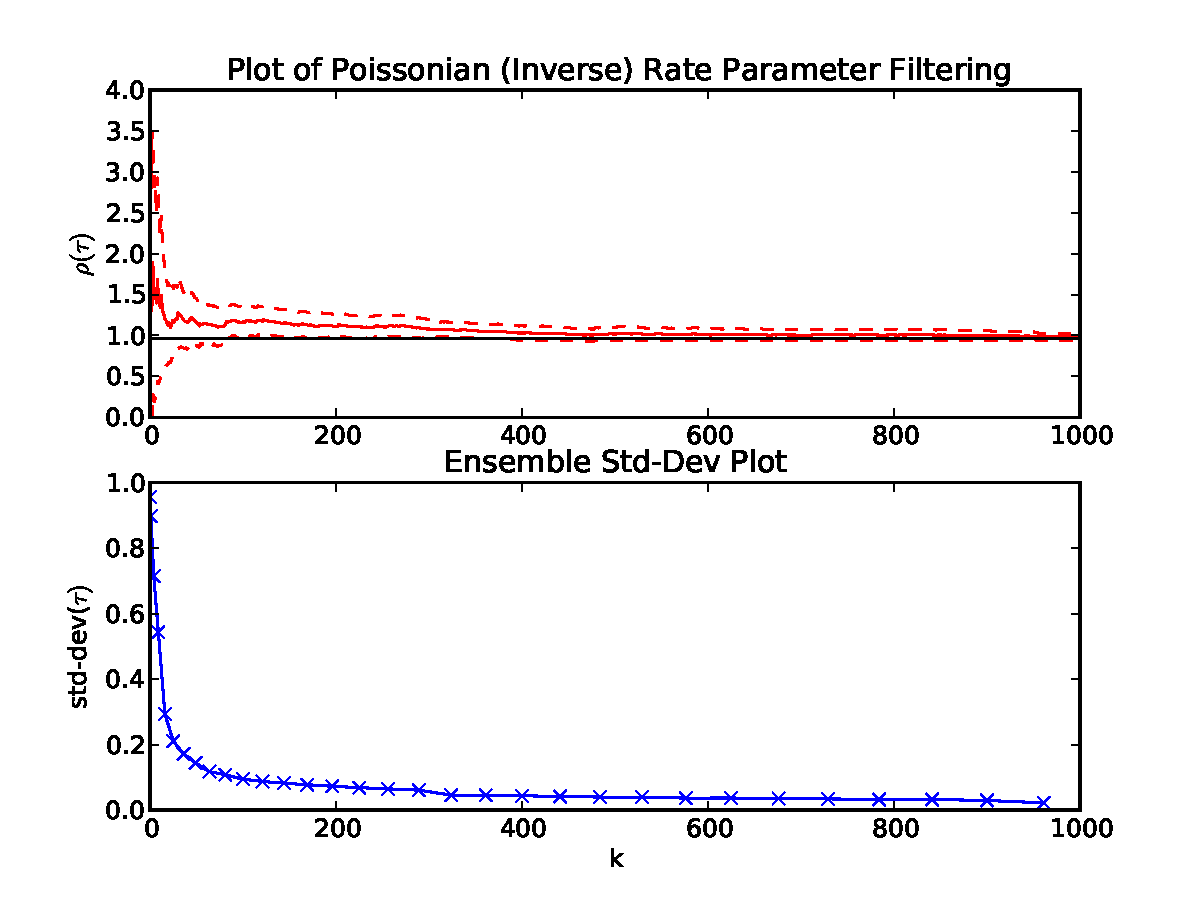
\includegraphics[width=\textwidth]{Figs/TauParticleEnsemble/poisson_rate_filtering.pdf}
%   \caption{Filtering Example for a test-case. We are trying to estimate the
%   inverse of the Poissonian rate, $1/\tau$, given inter-event intervals $t_k$.
%   The true value is $\tau  = 1$. The Maximum Likelihood estimate for $\tau$ in
%   this problem  is just the mean of the observed times $\bar{t_k}$, which
%   happens to be 0.9583 in this example, while after the last observation, the
%   ensemble mean $\pm$ std-dev is $0.9811\pm 0.0199$}
%   \label{fig:poissonian_rate_filtering}
% \end{center}
% \end{figure}

% \clearpage

\subsection{Simulation Results}
We now illustrate how the Optimal Design procedure works while using the
particle filtering methodology to represent and update our parameter prior.

% \subsubsection{Single Hitting-Time Illustration}
% In \cref{fig:example_online_miopt_single_iteration}, we
% illustrate one iteration of the update, that is one hitting time given a
% stimulation from either the MI Optimal Controller or a random controller, which
% just gives a random constant stimulation per each hitting time.
% 
% Let's discuss what happens in \cref{fig:example_online_miopt_single_iteration}.
% Recall that lower values of $\tc$ imply higher restoring force and therefore
% longer hitting times (waiting times). Since in this sample, the observed hitting
% times were fairly long, especially for the MI-optimal stimulation, weights for
% smaller $\t$s grow larger, while weights for bigger $\t$s become smaller.
% However it is immediately clear that the MI-optimal stimulation is more
% discerning as it has almost entirely discarded (correctly) the
% possibility that $\tau>2$, while the other two stimulations have resulted in
% only mild perturbation in the prior distribution. 
% 
% WARNING: The new results are much better primarily through a judicious choice of
% the initial condition of the MI-optimal optimization (the initial guess for the
% optimal control.)
% 
% \begin{figure}[h]
% \begin{center}
% \subfloat[Example Hitting Times]
% {
% \label{fig:example_hitting_times_for_online_miopt}
% \includegraphics[width=0.48\textwidth]
% {Figs/HTOnlineEstimator/single_trial_example_hittimes.pdf}
% } 
% \subfloat[Resulting Particle Ensemble Updates]
% {
% \label{fig:example_particle_ensemble_updates_for_online_miopt}
% \includegraphics[width=0.48\textwidth]
% {Figs/HTOnlineEstimator/single_trial_example_weights.pdf}
% }
% \caption[Effect of the First Observation on the Belief
% Distribution]{Examples of a single iteration of the Online Stimulation-Estimation scheme.}
% \label{fig:example_online_miopt_single_iteration}
% \end{center}
% \end{figure}
% 
% \subsubsection{Full Multiple Hitting-Times Experiment}
We stimulate a sequence
of hitting times and online update our parameter prior distribution, after
every observation and then online-update our MI-optimal stimulation as the
prior evolves. 

% The main result is shown in \cref{fig:example_miopt_vs_rand_ensemble_evolution},
% where we visualize the mean and confidence intervals for the belief
% distributions for the three protocols (MI-Optimal vs. Random Constant vs Zero),
% using $N_\t = 32$ particles and $N_k=251$ hitting times. In
% \cref{fig:example_miopt_controls_evolution}, we show the different stimulations
% that were chosen by the Mutual-Info Maximization Algorithm.
 
% \begin{figure}[htp]
% \begin{center}
%   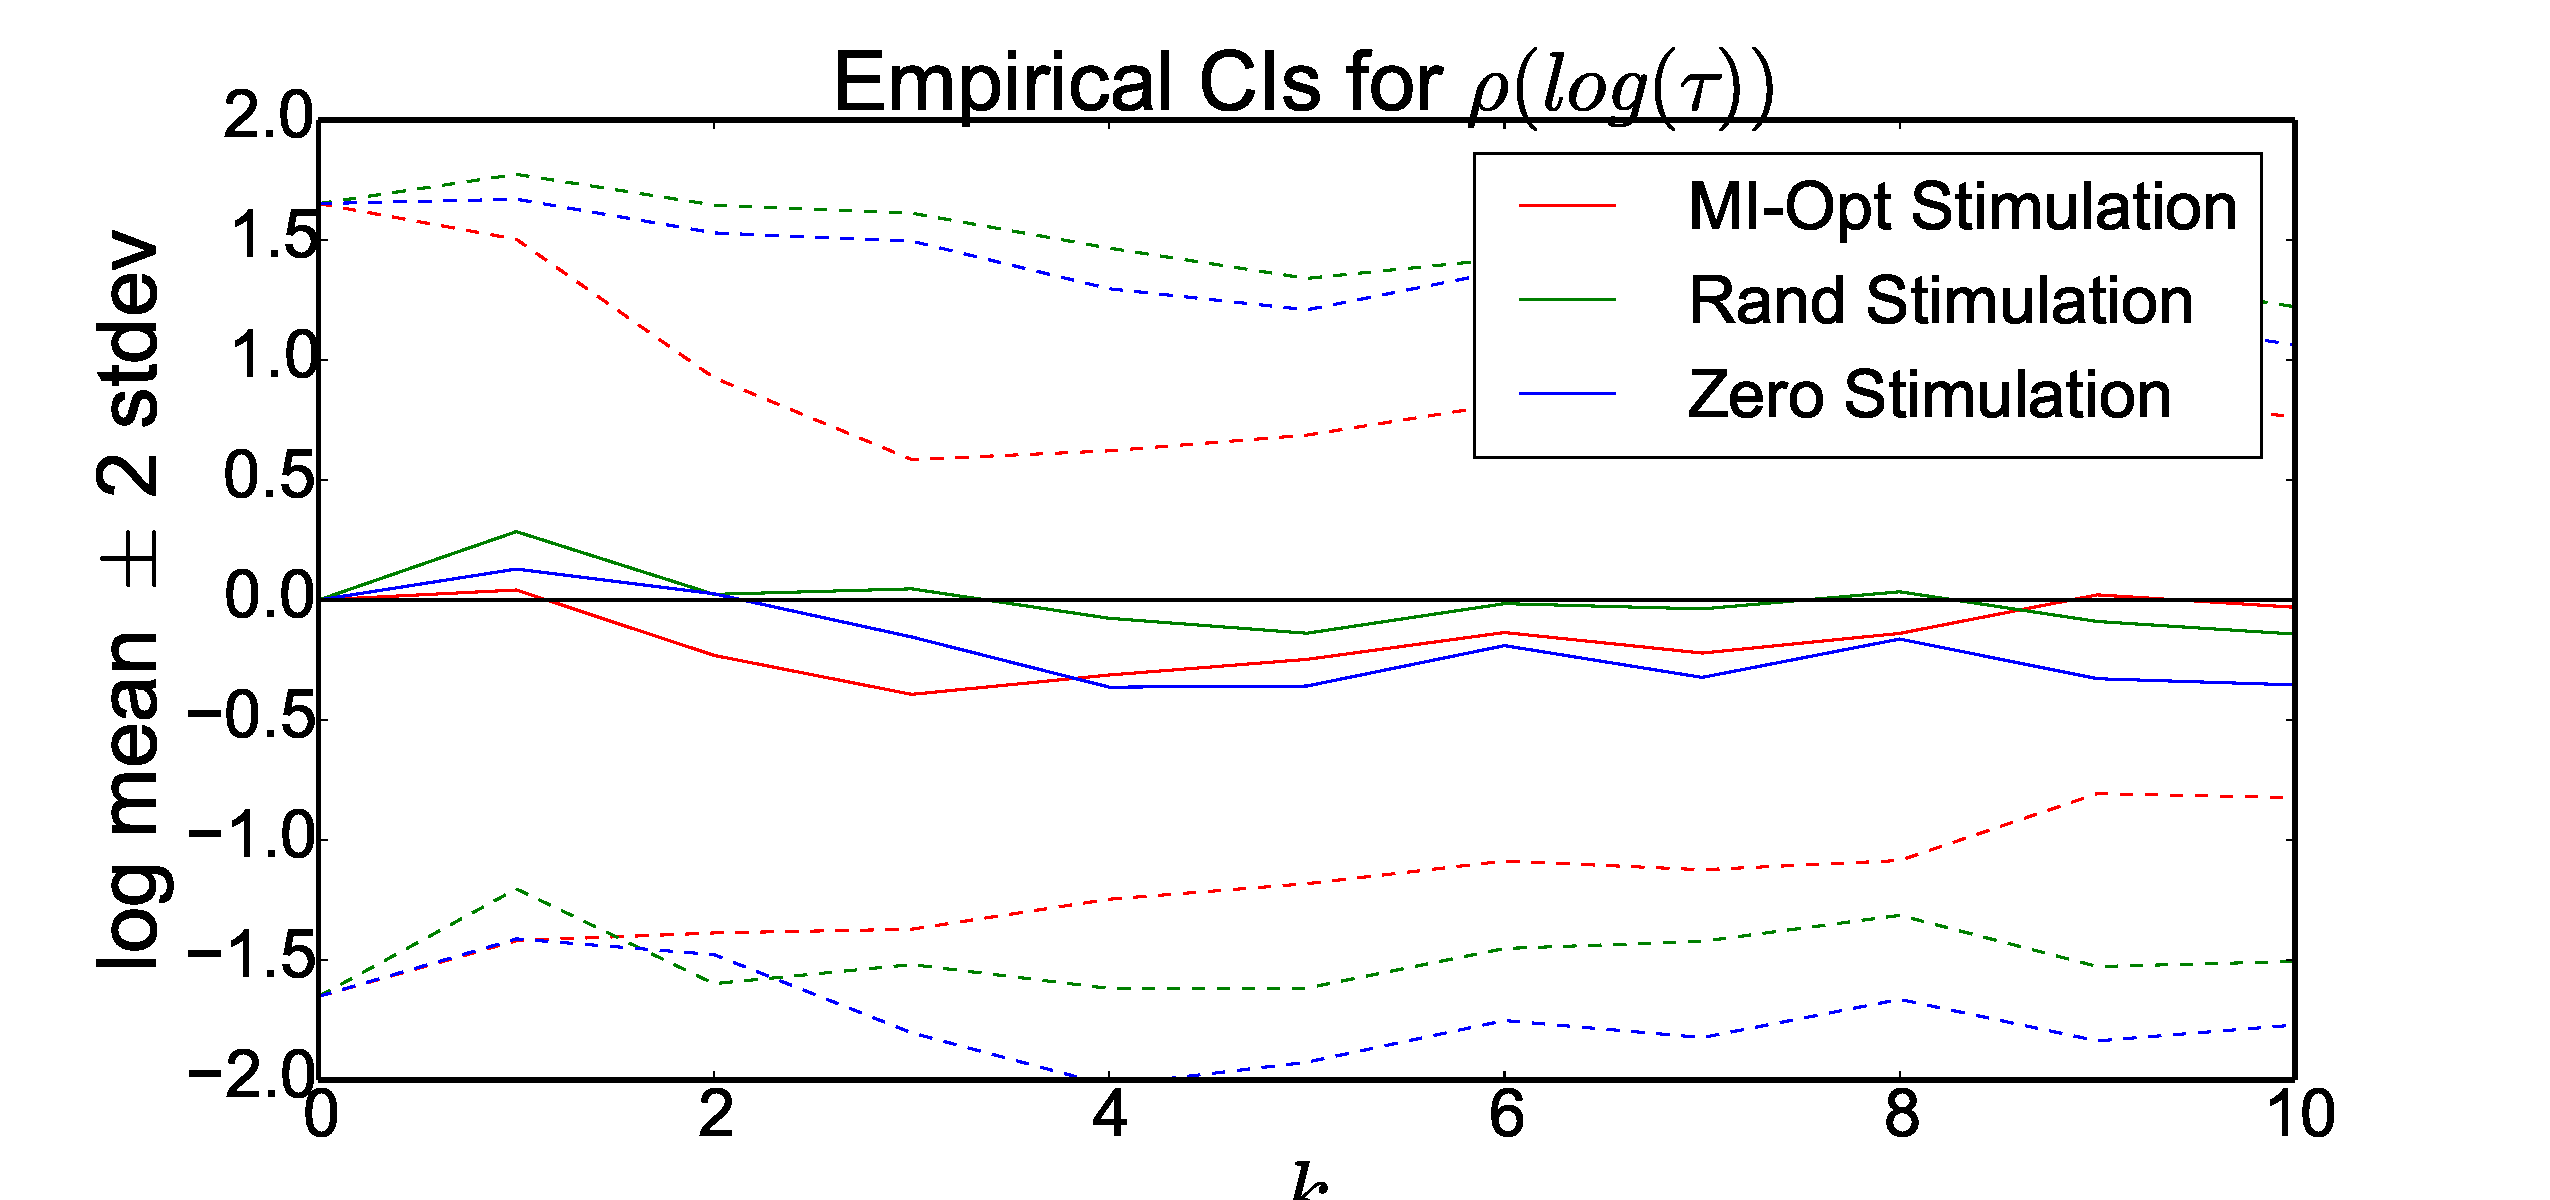
\includegraphics[width=\textwidth]{Figs/HTOnlineEstimator/single_experiment_example_ensemble_distn_evolution.pdf}
%   \caption[labelInTOC]{Evolution of the belief distributions given Optimal
%   (red) or Random (green) stimulation. We used $N=32$ particles to represent
%   the ensemble for both stimulation protocols. There are 250 hitting times used}
%   \label{fig:example_miopt_vs_rand_ensemble_evolution}
% \end{center}
% \end{figure}
% \begin{figure}[htp]
% \begin{center}
%   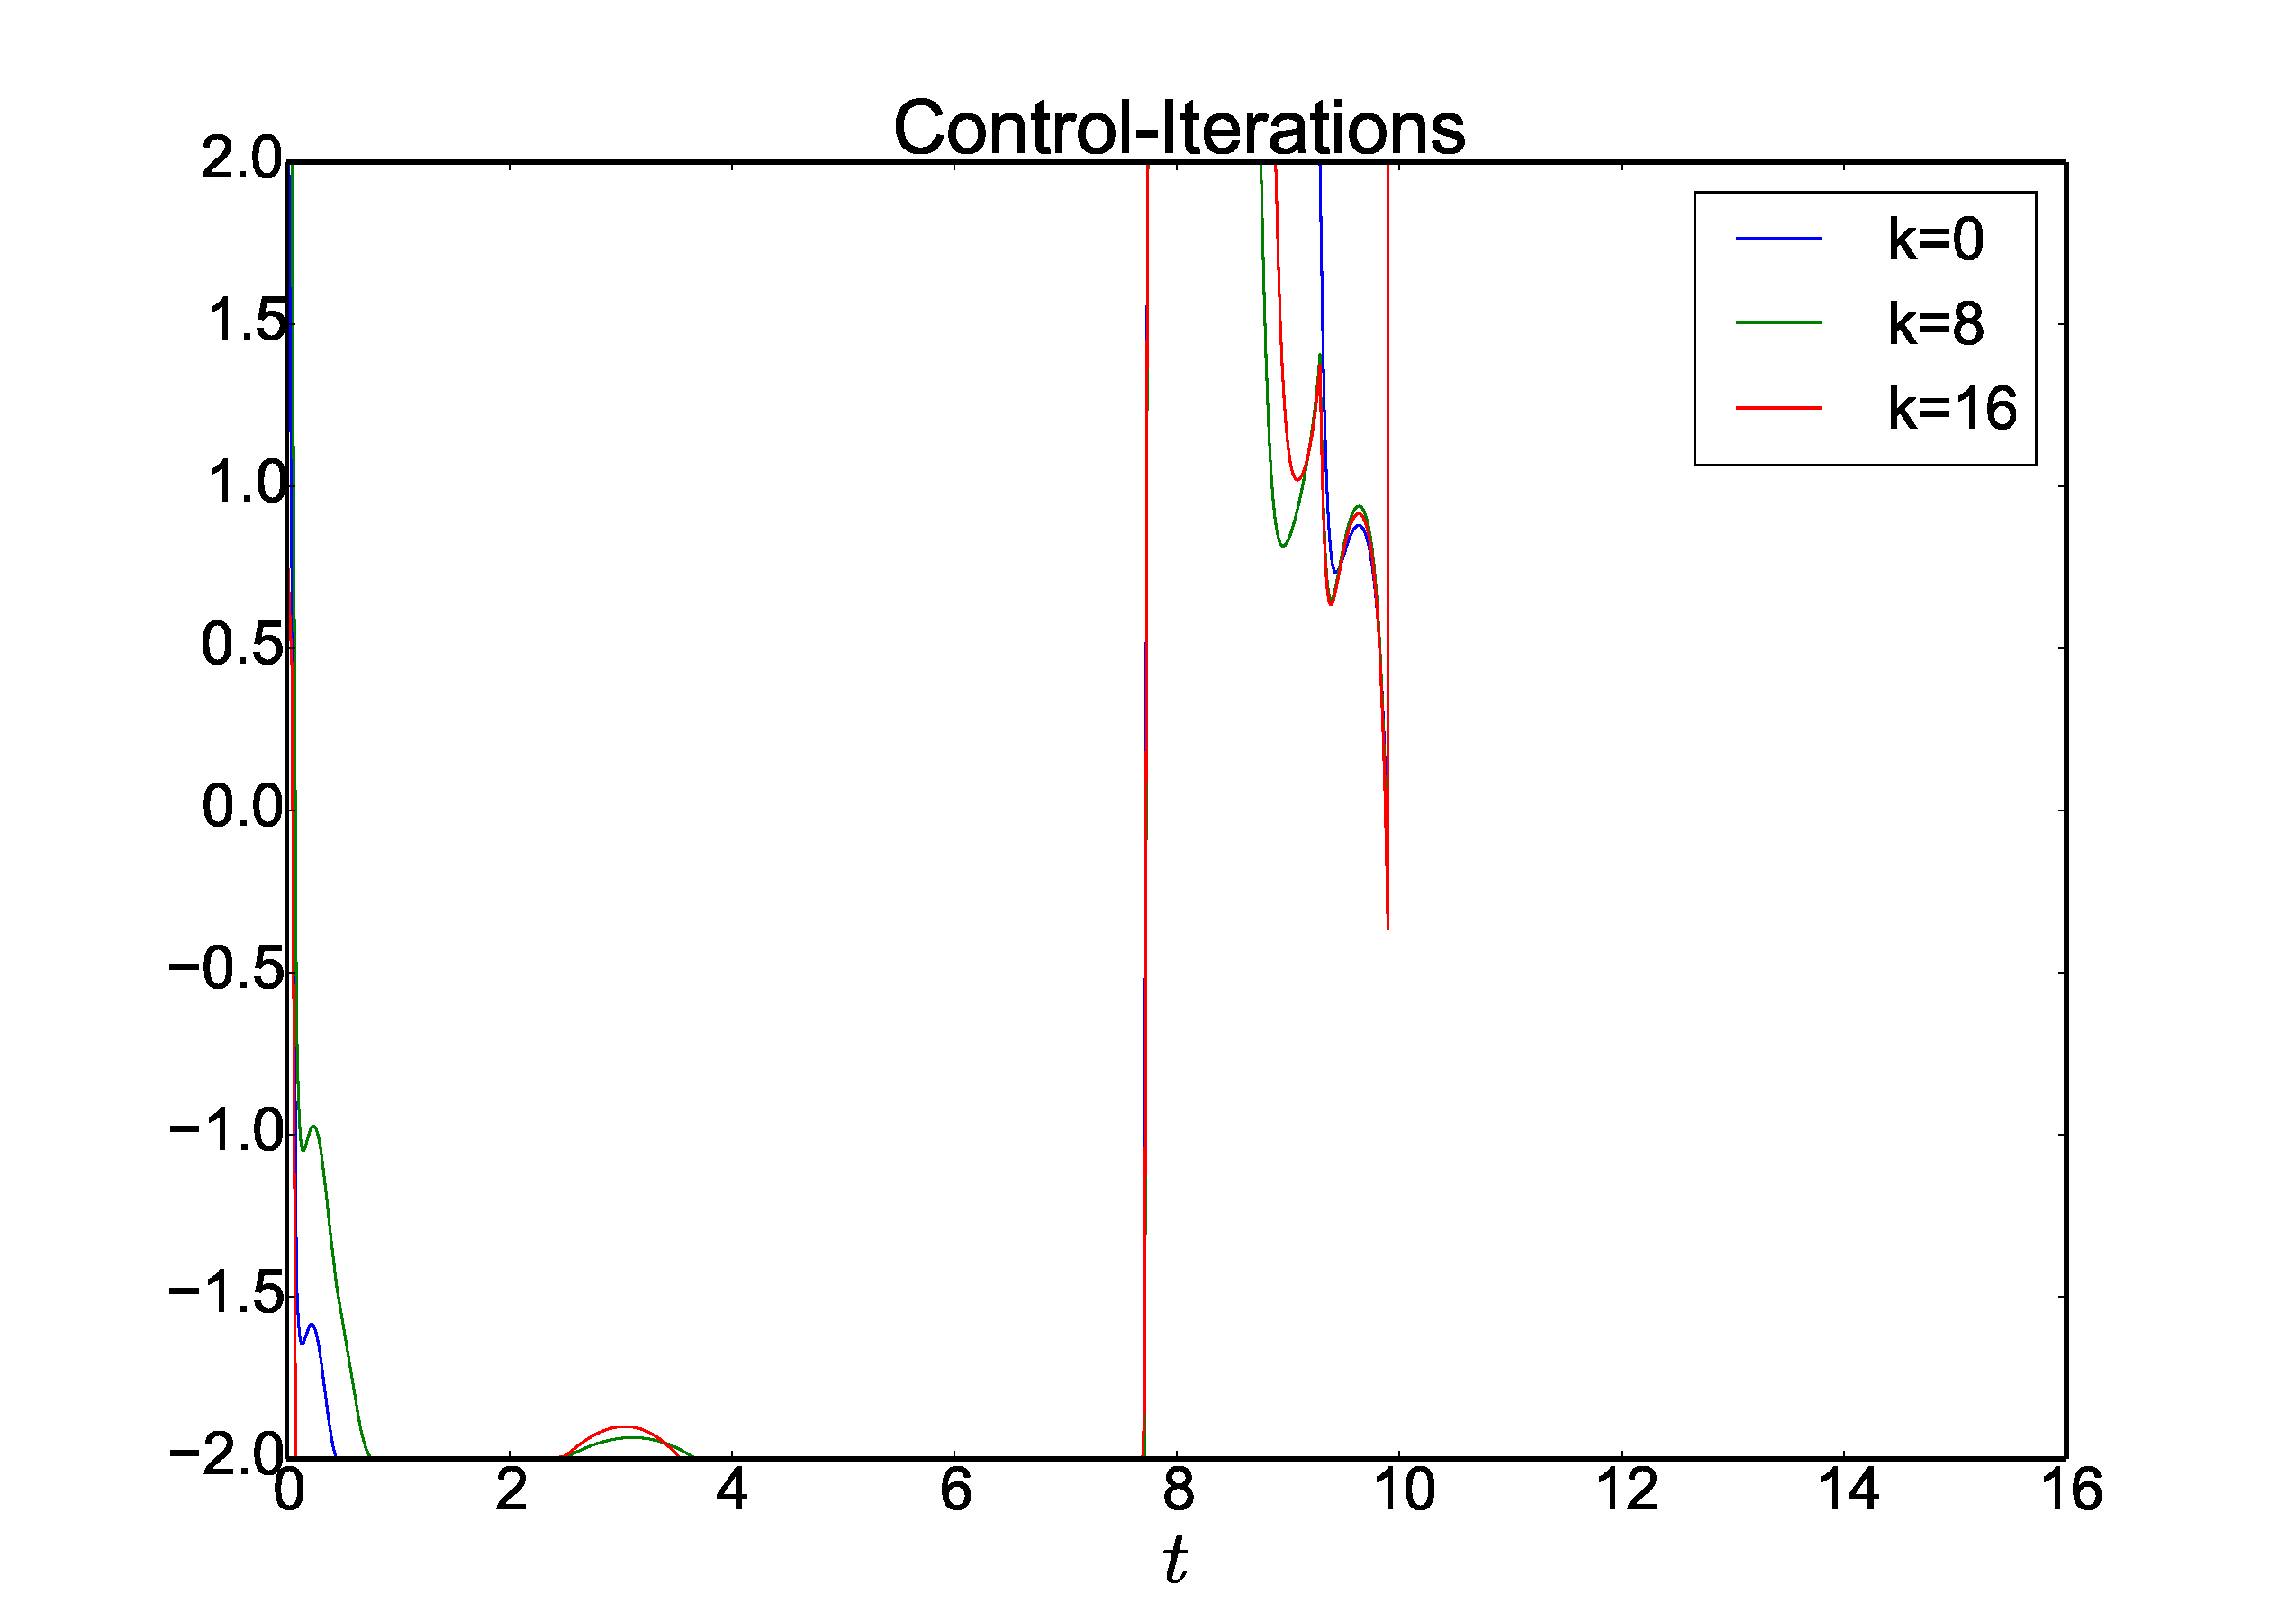
\includegraphics[width=\textwidth]{Figs/HTOnlineEstimator/single_experiment_example_controls_evolution.pdf}
%   \caption[labelInTOC]{Different MI-OPtimal Stimulations computed 
%   as the Experiment evolves and the parameter belief distribution changes}
%   \label{fig:example_miopt_controls_evolution}
% \end{center}
% \end{figure}
 
% \clearpage


We now simulate $50$ independent experiments of 500 hitting times each and
then average the ensembles.

% We visualize them in \cref{fig:online_optimization_more_examples}. Here, we
% see that the MI-optimal stimulation is indeed producing more accurate
% estimates, faster (earlier in the experiment). This is true in 7 out of the 10
% experiments, in 2 it is hard to determine whether there is a 'better' protocol
% and only once is the MI-based stimulation resulting in worse estimates than
% one of the alternatives ((f) in \cref{fig:online_optimization_more_examples}).
% \begin{figure}[h] \begin{center} \subfloat[] {
% \includegraphics[width=0.48\textwidth]
% {Figs/HTOnlineEstimator/single_experiment_exampleNts=32_Ntrls=495_ensemble_distn_evolution.pdf}
% } \subfloat[] { \includegraphics[width=0.48\textwidth]
% {Figs/HTOnlineEstimator/single_experiment_exampleNts=32_Ntrls=496_ensemble_distn_evolution.pdf}
% }\\
% \subfloat[] { \includegraphics[width=0.48\textwidth]
% {Figs/HTOnlineEstimator/single_experiment_exampleNts=32_Ntrls=497_ensemble_distn_evolution.pdf}
% } \subfloat[] { \includegraphics[width=0.48\textwidth]
% {Figs/HTOnlineEstimator/single_experiment_exampleNts=32_Ntrls=498_ensemble_distn_evolution.pdf}
% }\\
% \subfloat[] { \includegraphics[width=0.48\textwidth]
% {Figs/HTOnlineEstimator/single_experiment_exampleNts=32_Ntrls=499_ensemble_distn_evolution.pdf}
% } \subfloat[] { \includegraphics[width=0.48\textwidth]
% {Figs/HTOnlineEstimator/single_experiment_exampleNts=32_Ntrls=500_ensemble_distn_evolution.pdf}
% }\\
% \subfloat[] { \includegraphics[width=0.48\textwidth]
% {Figs/HTOnlineEstimator/single_experiment_exampleNts=32_Ntrls=501_ensemble_distn_evolution.pdf}
% } \subfloat[] { \includegraphics[width=0.48\textwidth]
% {Figs/HTOnlineEstimator/single_experiment_exampleNts=32_Ntrls=502_ensemble_distn_evolution.pdf}
% }\\
% \subfloat[] { \includegraphics[width=0.48\textwidth]
% {Figs/HTOnlineEstimator/single_experiment_exampleNts=32_Ntrls=503_ensemble_distn_evolution.pdf}
% } \subfloat[] { \includegraphics[width=0.48\textwidth]
% {Figs/HTOnlineEstimator/single_experiment_exampleNts=32_Ntrls=504_ensemble_distn_evolution.pdf}
% } \caption[labelInTOC]{Various examples of the perturbation-estimation
% protocol with the belief distribution plotted against the hitting time $k$,
% with the MI-optimal stimulation (red), the constant random stimulation (green)
% and the zero, $\a\equiv 0\,\forall t$, stimulation (blue)}
% \label{fig:online_optimization_more_examples} \end{center} \end{figure}
The aggregated evolutions for the updated prior distributions are
visualized in \cref{fig:online_optimization_aggregated_belief_evolution}. It is now clear that
the MI-Optimal procedure produces more accurate and more precise estiamtes and
that the increase in precision is especially clear in the earlier parts in the
experiment. That is, using the MI-optimal protocol reduces the uncertainty in
the parameters much faster.

In \cref{fig:online_optimization_quantiles_belief_evolution}, we plot a similar
illustration, here we show the median of the mean of the prior (median over the
$N=16$ experiments) as well as the min and the max. We see a similar effect in
that the 'opt'-estimates are much more accurate and precise. 

TODO: Should we include only one of these figs - they are kinda showing the
same thing?
 
% \usepackage{graphics} is needed for \includegraphics
\begin{figure}[htp]
\begin{center}
  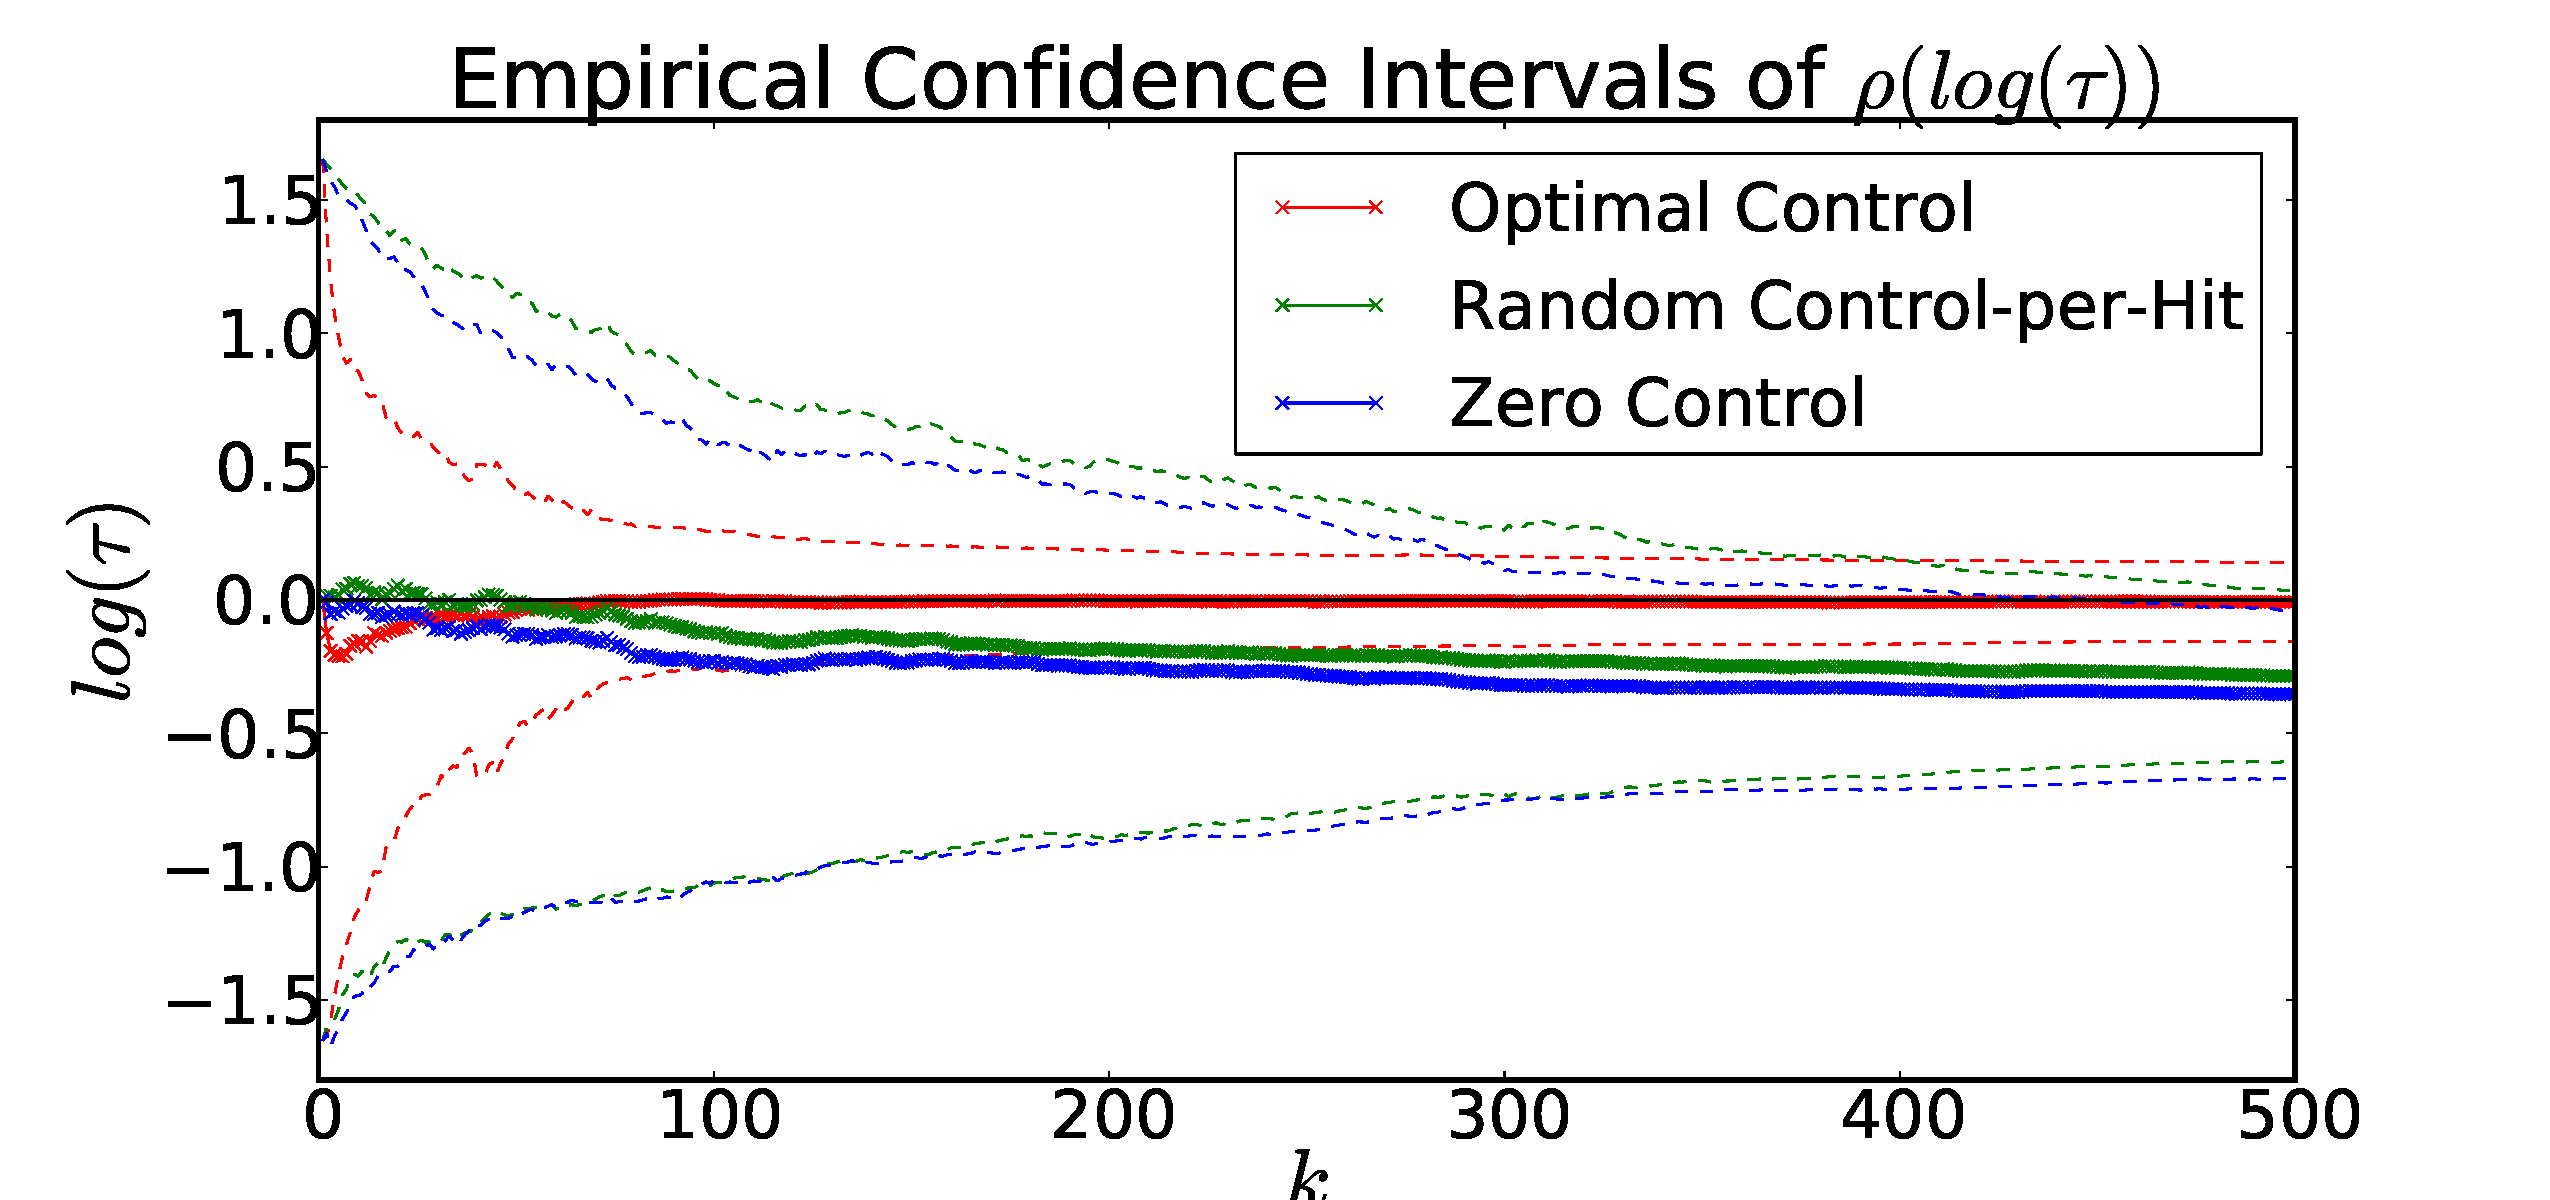
\includegraphics[width=\textwidth]{Figs/HTOnlineEstimator/online_updated_prior_mean_aggregated_ensemble.pdf}
  \caption[MI-Optimal Stimulation produces more precise parameter estimates]
  {MI-Optimal Stimulation produces more precise and more accurate parameter
  estimates. Visualized are the mean and confidence intervals for the parameter
  distribution of $\log (\tau)$, averaged over $N=50$ independent
  experiments. The black line indicates the 'true' value of the unknown parameter $\tau$.
  The solid (red,green and blue) lines indicate the mean of $\rho_{avg}$, while
  the dashed lines indicates 2 standard deviations in either direction of the
  mean. }  
  \label{fig:online_optimization_aggregated_belief_evolution}
\end{center}
\end{figure}

%\usepackage{graphics} is needed for \includegraphics
\begin{figure}[htp]
\begin{center}
  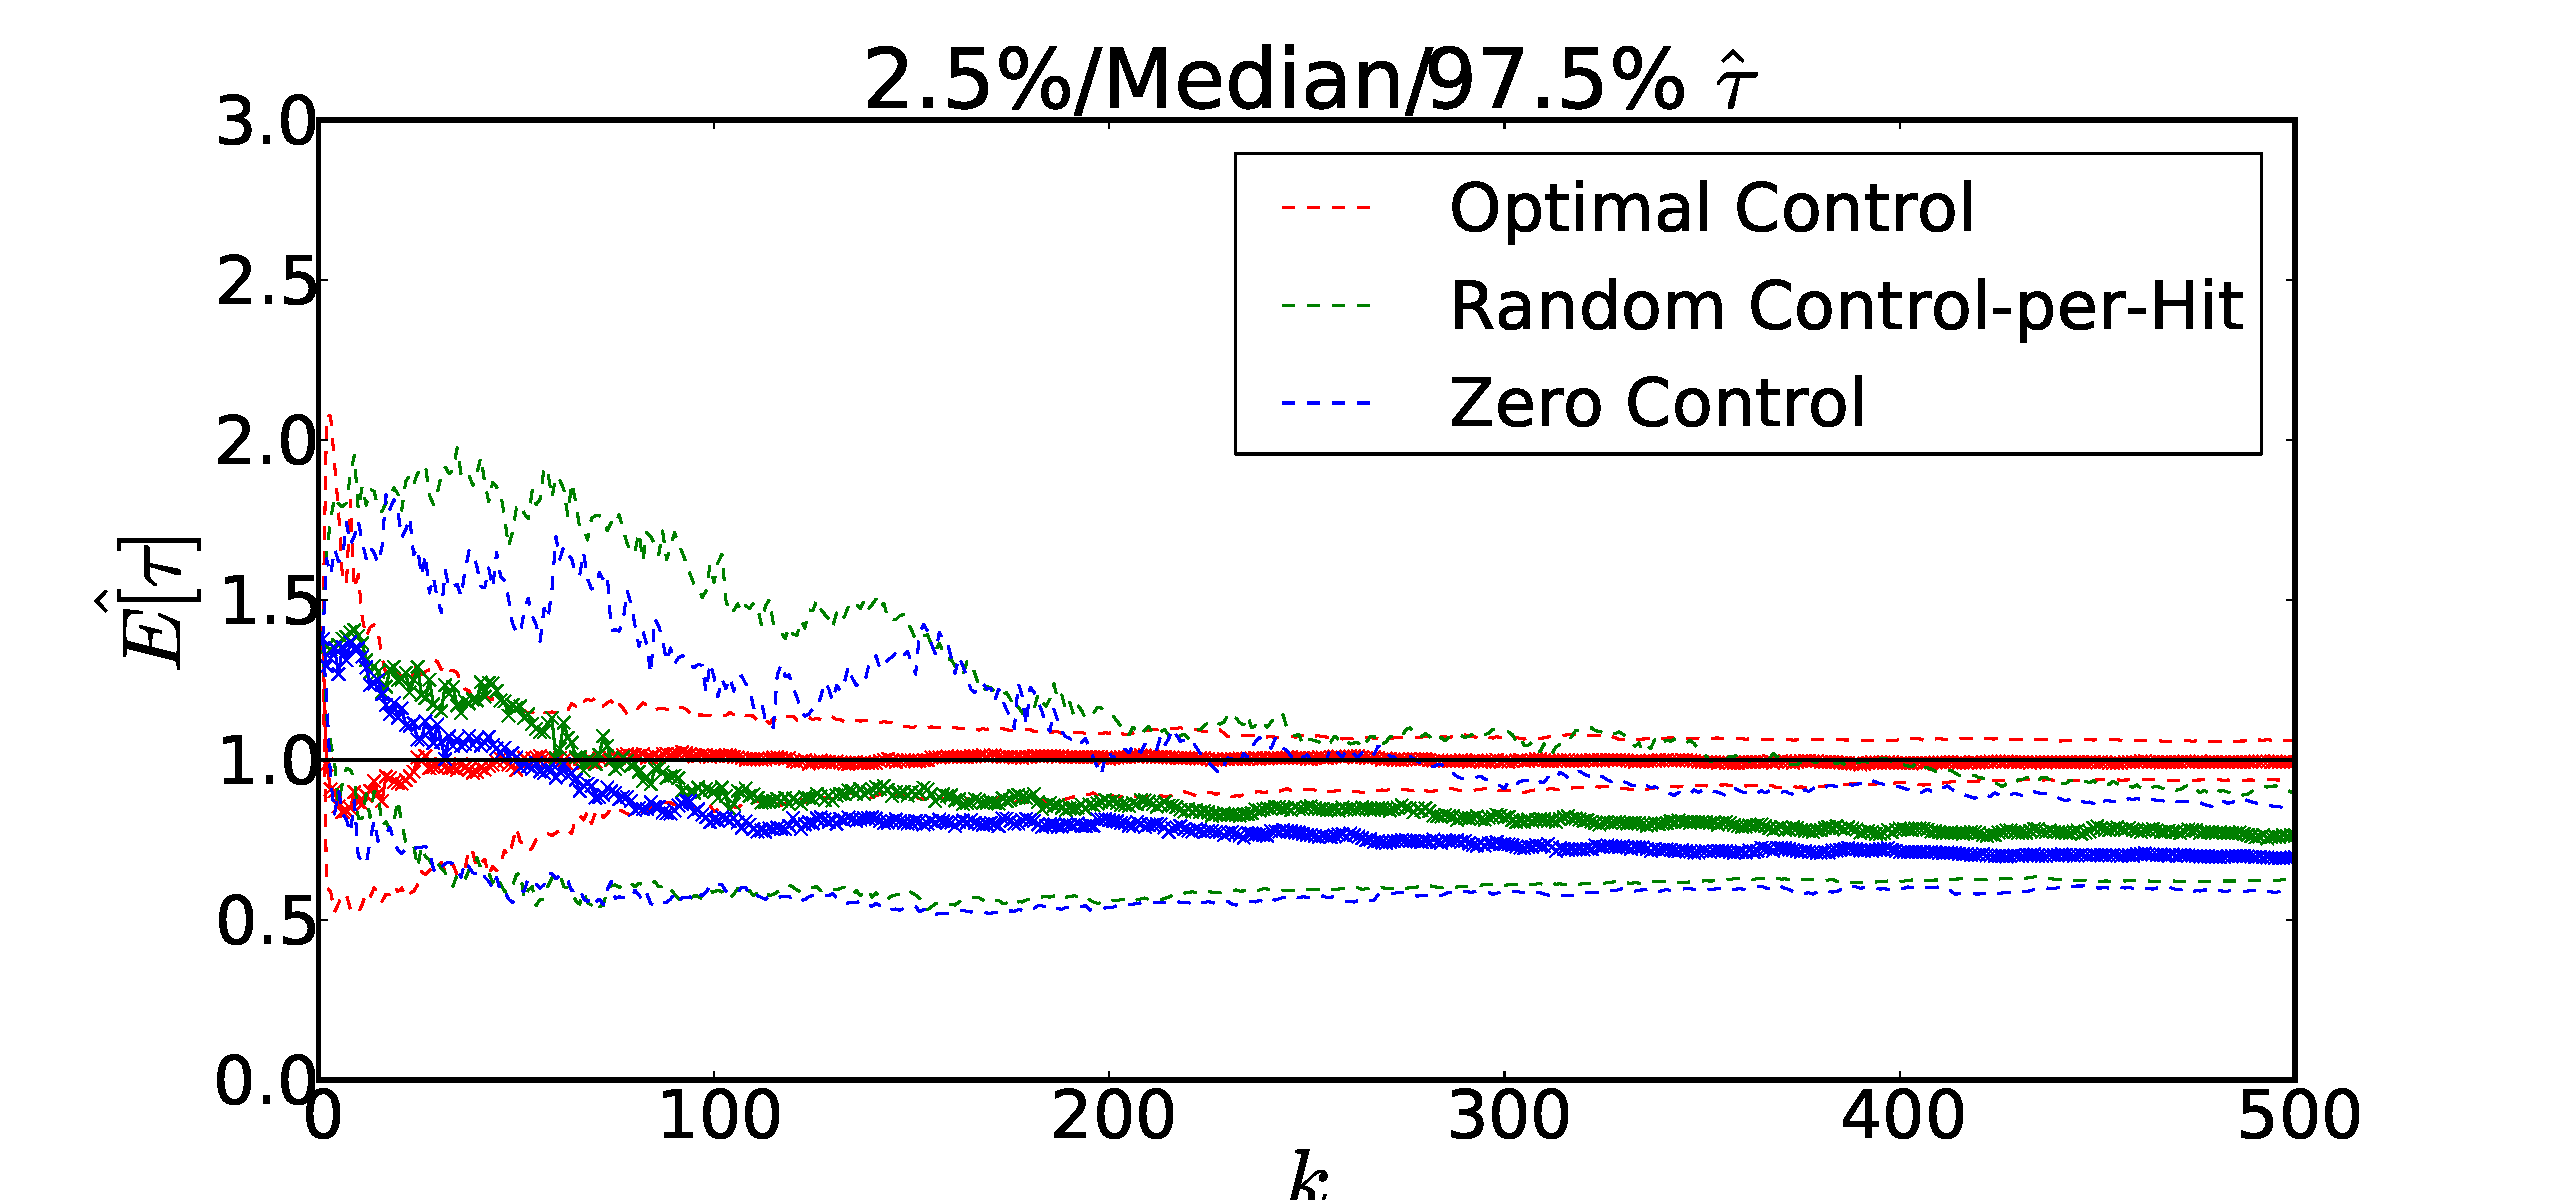
\includegraphics[width=\textwidth]{Figs/HTOnlineEstimator/online_updated_prior_quantiles_mean_per_experiment.pdf}
  \caption[Quantiles of the Mean Estimates]{Visualized are the median and
  2.5/97.5th percentiles of the mean of the updated prior
  distribution over the $N=50$ experiments. I.e.\ for each experiment and each
  hitting time, $k$, we compute the mean of the updated prior $\rho(\tc)$ and then we plot the median
  )crosses) of these means as well as the min and the max (dashes). Again we see
  that the median and the min/max of the optimally stimulated estimates are much closer to the
  true value of the parameter, $\tau$ then the estimates obtained from the
  naive stimulations.}
  \label{fig:online_optimization_quantiles_belief_evolution}
\end{center}
\end{figure}

\section{Discussion}
\label{sec:discussion}
We introduce a method for optimal design given hitting-time observations from a
Fokker-Planck system. Our method is based on maximizing the Mutual Information
between the observed hitting times and the parameter posterior distribution
of the parameters. The optimal control tends to separate
the hitting-time distributions associated with alternative values of the unknown
parameter, as such facilitating the identification of the parameter once an
observation is made. 

Our optimal stimulation selection uses PDE-based adjoint
optimization methods, which can be expensive and sensitive to the various
parameters of the optimization. 

The simulations show that the resulting estimates from the
optimally-stimulated system have higher precision and accuracy than sensible
alternatives, such as random stimulation or 'critical' stimulation or no
 stimulation at all.
 
TODO: WITHOUT BEING VERBOSE, GO OVER WHAT HAPPENED IN THE PAPER:)

Also compare with Existing Lit (e.g. Hooker paper)

Stress Novelty (of hitting time problem)
 

\clearpage
\section{Mutual Information definition}
\label{sec:mutual_info_defn} 

There are two standard references on Information Theory, 
\cite{Cover2006,MacKay2003}. The Mutual Information, $I$ between two random
variables, $X,Y$ is defined, for example, in Chapter 8 of \cite{MacKay2003},
where it says that $I(X,Y)$ represents the average reduction in uncertainty
about $x$ that results from learning the value of $y$ or vice versa! 

Here we show why our \cref{eq:J_mutual_info_objective} for the Mutual
Information agrees with the usual definition of the $I$,
which for the random variables, $X,\Theta$ is
\begin{equation} 
I(X,\Theta) = \int_\Theta \int_X p(x,\th) \cdot \log \left(
\frac{p(x,\th)}{p(x)p(\th)}\right) \intd{x} \intd{\th}
\label{eq:mutual_info_defn}
\end{equation}
 
First of all, the marginal distribution, $p(\th)$,  is just the prior of
$\Theta$, $$p(\th) = \rho(\th)$$ The joint distribution is $$p(x,y) =
L(x|\th)\rho(\th)$$ while the $X$ marginal is $$p(x) = \int_\Theta L(x|\th)\rho(\th) \intd{\th}$$
Plugging the three expressions into the definition in
\cref{eq:mutual_info_defn} gives:
\begin{equation}
I = \int_\Theta \int_X L(x|\th)\rho(\th) \cdot 
\log \left( \frac{L(x|\th)\rho(\th) }{\int_\Theta L(x|\th)\rho(\th) \intd{\th}
\cdot \rho(\th) } \right)
\intd{x}\intd{\th}.
\label{eq:mutual_info_prior_trajectory}
\end{equation}
And after canceling $\rho(\th)$ inside the $\log$, we get
\cref{eq:J_mutual_info_objective} .

\clearpage

\section{Pseudo-Code for Algorithms}
\begin{algorithm}
\begin{algorithmic}
\State Fix $\T, \ldots$ the problem parameters
\State Fix $\{t_n\}_0^{N_t}$ a time-discretization of $[0,\T]$
\State Fix $g_{tol}$ a convergence tolerance for the gradient
\State Fix $K_{\max}, I_{\max}$ number of maximum iterations in outer, inner
loops
\State Fix $s$ the initial step-size. 
\\ {\itshape $\#$ we use $g_{tol}=1e-5,K_{\max}=100,I_{\max}=10,s=10$}
\State $\a_1(t) \gets (\amax-\amin) \cdot t / \T + \amin$ 
\\{\itshape  $\#$ $\a_1(t) \sim$ initial guess for the control, linear
interpolate between $\amin, \amax$}
\For { $k= 1\dots K_{\max}$} 
\\ {\itshape $\#$ This is the outer loop where we descend down different
gradients}
 \State Calculate $f_k,I_{k},p_k, \delta_\a I_k$ corresponding to
	$\a_k$ from
	\cref{eq:hamiltonian_gradient,eq:adjoint_pde_OU,eq:FP_pde_OU_PDF,eq:OC_LS_variance_density}
	\State $N_{active}\gets$   Number of time nodes $t_n$, where either
	$\a_k(t_n) \neq \{\amin, \amax\}$ or $\delta_\a I_k(t_n)$ points inwards
	\If{ $|| \delta_\a I_k||_{\R^{N_{active}}} \leq g_{tol}\cdot N_{active}$}
		  \\ {\itshape  $\#$ 'Active' gradient is small enough,
		 consider converged:}
		 \State BREAK
	\EndIf
	\\ {\itshape $\#$ Find the step size, $s$, of how far to move $\a$ in the
	direction $\delta_\a I_k$:}
	\For { $j= 1\dots K_{\max}$}
	\\ {\itshape $\#$ This is the inner loop where we find how much to descend down
	the current gradient}
	\State $\a_{k,j} \gets \a_{k} + s_j \cdot \delta_\a I_k  $
	\\ {\itshape $\#$ $\a_{k,j}$ is the new control strategy to try}
	\State Calculate $f_{\th,k,j}, I_{k,j}$ corresponding to
		$\a_{k,j}$ from
		\cref{eq:FP_pde_OU_absorbBC,eq:I_mutual_info_objective_in_terms_of_dixf} \\
		{\itshape $\#$ Recall $f_{\th,k,j}$ is a probability density resulting from
		the control $a_{k,j}$ and $I_{k,j}$ is the objective value resulting from $f_{k,j}$}  
	\If {$I_{k,j} < I_k$}
		\\ {\itshape $\#$ We found a better (smaller) objective value}
		\State $s \gets 2 s_j$ {\itshape $\#$ start from a more aggressive step in the
		next iteration}
		\State BREAK
		\EndIf
	\If {$j == J_{\max}$}
		\\ {\itshape $\#$ We exhausted the step search without finding a 
		smaller $I$, return current values}
		\State Return $I_k, \a_k$
	\EndIf
 	\\ {\itshape  $ \#$ Continue inner loop, try a smaller step:}
	 	\State $s_{j+1}  \gets  s_j / 2$
    \EndFor  {\itshape $\quad \#$ single step loop}
	\If {$k == K_{\max}$}
		\State ERROR 'Could not converge'
	\EndIf
    \\{\itshape $\#$ Assign the new candidate for the optimal control and
    re-loop}
		\State $\a_{k+1} \gets \a_{k,j}$
\EndFor {\itshape $\quad \#$ gradient ascent loop}
\State \Return $J_k, \a_k$
\end{algorithmic}
\caption{Gradient ascent algorithm for obtaining the optimal open-loop 
control}
\label{alg:gradient_ascent_4_OC}
\end{algorithm}

\clearpage 


\begin{algorithm}
\begin{algorithmic}
\State Given  $\{w_i, \th_i\}_1^N_p$ the current particle ensemble (weight,
locations)  
\\ {\itshape $\#$ Observe a single hitting-time, $t_k$ from the real (or
simulated) system conditional on the applied control $\a_k(\cdot)$}
\\ {\itshape $\#$ Update weights with likelihood given $t_k$ and normalize:}
\State $w_{i } \gets w_{i }\cdot g(t_k| \th_i, \a_k)$
\State $w_{i } \gets w_{i }/ \sum w_i$
\If{$$\frac{1}{\sum_i^{N_p} w_i^2} < \frac {N_p}{2}$$} 
\\ {\itshape $\#$ Re-sample the ensemble:}
\State $\m $ \gets
$\Exp[\Th] = \sum w_i \th_i$ 
\State $a = 0.98$, see
\cite{Granade2012,Liu2001} 
\State $h = \sqrt{1-a^2}$ i.e. $h \approx 0.1990$
\State $\Xi$\gets $h^2\cdot \Var[\Th]$
	\\ {\itshape $\#$ Re-sample each particle individually:}
\For {$i= 1\dots N_p$}
	\State draw $j$ with probability $w_j$ 
% 	\\ {\itshape $\#$ the bigger $w_i$ the more likely to choose
% 	$\th_i$}
	\State $\m_i$ \gets  $a \th_j + (1-a) \m$
	\State Resample $\th_i$ from $N(\m_i, \Xi)$
	\State $w_i$ \gets $1/N_p$ 
    \EndFor{\itshape $\quad \#   1 \ldots N_p$ particle resampling}
    \EndIf{\itshape Conditional Resampling}
\State \Return $w_i, \th_i$ the updated and possibly-resampled particle
ensemble
\end{algorithmic}
\caption{Particle Filtering for Parameter Estimation}
\label{alg:particle_resampling}
\end{algorithm}

\section{Code Repository}
All the code used in the paper including code to generate the figures can be
found on
\href{https://github.com/aviolov/OptEstimatePython}{github @
https://github.com/aviolov/OptEstimatePython}. Please contact the first author
for furhter information.



\section{Extra Stuff}
TODO: Move all discussion of Double WEll here\ldots


 
\clearpage